% Options for packages loaded elsewhere
%DIF LATEXDIFF DIFFERENCE FILE
%DIF DEL old.Revell.phytools-v2_peerj.tex   Thu Aug  3 14:05:32 2023
%DIF ADD Revell.phytools-v2_peerj.tex       Thu Aug  3 14:06:15 2023
\PassOptionsToPackage{unicode}{hyperref}
\PassOptionsToPackage{hyphens}{url}
%

\documentclass[fleqn,10pt,lineno]{wlpeerj}
\usepackage{amsmath,amssymb}
\usepackage{iftex}
\ifPDFTeX
  \usepackage[T1]{fontenc}
  \usepackage[utf8]{inputenc}
  \usepackage{textcomp} % provide euro and other symbols
\else % if luatex or xetex
  \usepackage{unicode-math} % this also loads fontspec
  \defaultfontfeatures{Scale=MatchLowercase}
  \defaultfontfeatures[\rmfamily]{Ligatures=TeX,Scale=1}
\fi
\usepackage{lmodern}
\ifPDFTeX\else
  % xetex/luatex font selection
\fi
% Use upquote if available, for straight quotes in verbatim environments
\IfFileExists{upquote.sty}{\usepackage{upquote}}{}
\IfFileExists{microtype.sty}{% use microtype if available
  \usepackage[]{microtype}
  \UseMicrotypeSet[protrusion]{basicmath} % disable protrusion for tt fonts
}{}
\makeatletter
\@ifundefined{KOMAClassName}{% if non-KOMA class
  \IfFileExists{parskip.sty}{%
    \usepackage{parskip}
  }{% else
    \setlength{\parindent}{0pt}
    \setlength{\parskip}{6pt plus 2pt minus 1pt}}
}{% if KOMA class
  \KOMAoptions{parskip=half}}
\makeatother
\usepackage{xcolor}
\usepackage[margin=1in]{geometry}
\usepackage{color}
\usepackage{fancyvrb}
\newcommand{\VerbBar}{|}
\newcommand{\VERB}{\Verb[commandchars=\\\{\}]}
\DefineVerbatimEnvironment{Highlighting}{Verbatim}{commandchars=\\\{\}}
% Add ',fontsize=\small' for more characters per line
\usepackage{framed}
\definecolor{shadecolor}{RGB}{248,248,248}
\newenvironment{Shaded}{\begin{snugshade}}{\end{snugshade}}
\newcommand{\AlertTok}[1]{\textcolor[rgb]{0.94,0.16,0.16}{#1}}
\newcommand{\AnnotationTok}[1]{\textcolor[rgb]{0.56,0.35,0.01}{\textbf{\textit{#1}}}}
\newcommand{\AttributeTok}[1]{\textcolor[rgb]{0.13,0.29,0.53}{#1}}
\newcommand{\BaseNTok}[1]{\textcolor[rgb]{0.00,0.00,0.81}{#1}}
\newcommand{\BuiltInTok}[1]{#1}
\newcommand{\CharTok}[1]{\textcolor[rgb]{0.31,0.60,0.02}{#1}}
\newcommand{\CommentTok}[1]{\textcolor[rgb]{0.56,0.35,0.01}{\textit{#1}}}
\newcommand{\CommentVarTok}[1]{\textcolor[rgb]{0.56,0.35,0.01}{\textbf{\textit{#1}}}}
\newcommand{\ConstantTok}[1]{\textcolor[rgb]{0.56,0.35,0.01}{#1}}
\newcommand{\ControlFlowTok}[1]{\textcolor[rgb]{0.13,0.29,0.53}{\textbf{#1}}}
\newcommand{\DataTypeTok}[1]{\textcolor[rgb]{0.13,0.29,0.53}{#1}}
\newcommand{\DecValTok}[1]{\textcolor[rgb]{0.00,0.00,0.81}{#1}}
\newcommand{\DocumentationTok}[1]{\textcolor[rgb]{0.56,0.35,0.01}{\textbf{\textit{#1}}}}
\newcommand{\ErrorTok}[1]{\textcolor[rgb]{0.64,0.00,0.00}{\textbf{#1}}}
\newcommand{\ExtensionTok}[1]{#1}
\newcommand{\FloatTok}[1]{\textcolor[rgb]{0.00,0.00,0.81}{#1}}
\newcommand{\FunctionTok}[1]{\textcolor[rgb]{0.13,0.29,0.53}{\textbf{#1}}}
\newcommand{\ImportTok}[1]{#1}
\newcommand{\InformationTok}[1]{\textcolor[rgb]{0.56,0.35,0.01}{\textbf{\textit{#1}}}}
\newcommand{\KeywordTok}[1]{\textcolor[rgb]{0.13,0.29,0.53}{\textbf{#1}}}
\newcommand{\NormalTok}[1]{#1}
\newcommand{\OperatorTok}[1]{\textcolor[rgb]{0.81,0.36,0.00}{\textbf{#1}}}
\newcommand{\OtherTok}[1]{\textcolor[rgb]{0.56,0.35,0.01}{#1}}
\newcommand{\PreprocessorTok}[1]{\textcolor[rgb]{0.56,0.35,0.01}{\textit{#1}}}
\newcommand{\RegionMarkerTok}[1]{#1}
\newcommand{\SpecialCharTok}[1]{\textcolor[rgb]{0.81,0.36,0.00}{\textbf{#1}}}
\newcommand{\SpecialStringTok}[1]{\textcolor[rgb]{0.31,0.60,0.02}{#1}}
\newcommand{\StringTok}[1]{\textcolor[rgb]{0.31,0.60,0.02}{#1}}
\newcommand{\VariableTok}[1]{\textcolor[rgb]{0.00,0.00,0.00}{#1}}
\newcommand{\VerbatimStringTok}[1]{\textcolor[rgb]{0.31,0.60,0.02}{#1}}
\newcommand{\WarningTok}[1]{\textcolor[rgb]{0.56,0.35,0.01}{\textbf{\textit{#1}}}}
\usepackage{graphicx}
\makeatletter
\def\maxwidth{\ifdim\Gin@nat@width>\linewidth\linewidth\else\Gin@nat@width\fi}
\def\maxheight{\ifdim\Gin@nat@height>\textheight\textheight\else\Gin@nat@height\fi}
\makeatother
% Scale images if necessary, so that they will not overflow the page
% margins by default, and it is still possible to overwrite the defaults
% using explicit options in \includegraphics[width, height, ...]{}
\setkeys{Gin}{width=\maxwidth,height=\maxheight,keepaspectratio}
% Set default figure placement to htbp
\makeatletter
\def\fps@figure{htbp}
\makeatother
\setlength{\emergencystretch}{3em} % prevent overfull lines
\providecommand{\tightlist}{%
  \setlength{\itemsep}{0pt}\setlength{\parskip}{0pt}}
\setcounter{secnumdepth}{-\maxdimen} % remove section numbering
\newlength{\cslhangindent}
\setlength{\cslhangindent}{1.5em}
\newlength{\csllabelwidth}
\setlength{\csllabelwidth}{3em}
\newlength{\cslentryspacingunit} % times entry-spacing
\setlength{\cslentryspacingunit}{\parskip}
\newenvironment{CSLReferences}[2] % #1 hanging-ident, #2 entry spacing
 {% don't indent paragraphs
  \setlength{\parindent}{0pt}
  % turn on hanging indent if param 1 is 1
  \ifodd #1
  \let\oldpar\par
  \def\par{\hangindent=\cslhangindent\oldpar}
  \fi
  % set entry spacing
  \setlength{\parskip}{#2\cslentryspacingunit}
 }%
 {}
\usepackage{calc}
\newcommand{\CSLBlock}[1]{#1\hfill\break}
\newcommand{\CSLLeftMargin}[1]{\parbox[t]{\csllabelwidth}{#1}}
\newcommand{\CSLRightInline}[1]{\parbox[t]{\linewidth - \csllabelwidth}{#1}\break}
\newcommand{\CSLIndent}[1]{\hspace{\cslhangindent}#1}
\usepackage{fancyhdr}
\pagestyle{fancy}
\fancyhead[L]{Revell, L. J. (2023)}
\fancyhead[C]{}
\fancyhead[R]{phytools 2.0}

\ifLuaTeX
  \usepackage{selnolig}  % disable illegal ligatures
\fi
\IfFileExists{bookmark.sty}{\usepackage{bookmark}}{\usepackage{hyperref}}
\IfFileExists{xurl.sty}{\usepackage{xurl}}{} % add URL line breaks if available
\urlstyle{same}
\hypersetup{
  pdftitle={phytools 2.0: An updated R ecosystem for phylogenetic comparative methods (and other things)},
  hidelinks,
  pdfcreator={LaTeX via pandoc}}

\title{phytools 2.0: An updated R ecosystem for phylogenetic comparative
methods (and other things)}
\author{true}
\date{}
%DIF PREAMBLE EXTENSION ADDED BY LATEXDIFF
%DIF UNDERLINE PREAMBLE %DIF PREAMBLE
\RequirePackage[normalem]{ulem} %DIF PREAMBLE
\RequirePackage{color}\definecolor{RED}{rgb}{1,0,0}\definecolor{BLUE}{rgb}{0,0,1} %DIF PREAMBLE
\providecommand{\DIFaddtex}[1]{{\protect\color{blue}\uwave{#1}}} %DIF PREAMBLE
\providecommand{\DIFdeltex}[1]{{\protect\color{red}\sout{#1}}}                      %DIF PREAMBLE
%DIF SAFE PREAMBLE %DIF PREAMBLE
\providecommand{\DIFaddbegin}{} %DIF PREAMBLE
\providecommand{\DIFaddend}{} %DIF PREAMBLE
\providecommand{\DIFdelbegin}{} %DIF PREAMBLE
\providecommand{\DIFdelend}{} %DIF PREAMBLE
\providecommand{\DIFmodbegin}{} %DIF PREAMBLE
\providecommand{\DIFmodend}{} %DIF PREAMBLE
%DIF FLOATSAFE PREAMBLE %DIF PREAMBLE
\providecommand{\DIFaddFL}[1]{\DIFadd{#1}} %DIF PREAMBLE
\providecommand{\DIFdelFL}[1]{\DIFdel{#1}} %DIF PREAMBLE
\providecommand{\DIFaddbeginFL}{} %DIF PREAMBLE
\providecommand{\DIFaddendFL}{} %DIF PREAMBLE
\providecommand{\DIFdelbeginFL}{} %DIF PREAMBLE
\providecommand{\DIFdelendFL}{} %DIF PREAMBLE
%DIF HYPERREF PREAMBLE %DIF PREAMBLE
\providecommand{\DIFadd}[1]{\texorpdfstring{\DIFaddtex{#1}}{#1}} %DIF PREAMBLE
\providecommand{\DIFdel}[1]{\texorpdfstring{\DIFdeltex{#1}}{}} %DIF PREAMBLE
\newcommand{\DIFscaledelfig}{0.5}
%DIF HIGHLIGHTGRAPHICS PREAMBLE %DIF PREAMBLE
\RequirePackage{settobox} %DIF PREAMBLE
\RequirePackage{letltxmacro} %DIF PREAMBLE
\newsavebox{\DIFdelgraphicsbox} %DIF PREAMBLE
\newlength{\DIFdelgraphicswidth} %DIF PREAMBLE
\newlength{\DIFdelgraphicsheight} %DIF PREAMBLE
% store original definition of \includegraphics %DIF PREAMBLE
\LetLtxMacro{\DIFOincludegraphics}{\includegraphics} %DIF PREAMBLE
\newcommand{\DIFaddincludegraphics}[2][]{{\color{blue}\fbox{\DIFOincludegraphics[#1]{#2}}}} %DIF PREAMBLE
\newcommand{\DIFdelincludegraphics}[2][]{% %DIF PREAMBLE
\sbox{\DIFdelgraphicsbox}{\DIFOincludegraphics[#1]{#2}}% %DIF PREAMBLE
\settoboxwidth{\DIFdelgraphicswidth}{\DIFdelgraphicsbox} %DIF PREAMBLE
\settoboxtotalheight{\DIFdelgraphicsheight}{\DIFdelgraphicsbox} %DIF PREAMBLE
\scalebox{\DIFscaledelfig}{% %DIF PREAMBLE
\parbox[b]{\DIFdelgraphicswidth}{\usebox{\DIFdelgraphicsbox}\\[-\baselineskip] \rule{\DIFdelgraphicswidth}{0em}}\llap{\resizebox{\DIFdelgraphicswidth}{\DIFdelgraphicsheight}{% %DIF PREAMBLE
\setlength{\unitlength}{\DIFdelgraphicswidth}% %DIF PREAMBLE
\begin{picture}(1,1)% %DIF PREAMBLE
\thicklines\linethickness{2pt} %DIF PREAMBLE
{\color[rgb]{1,0,0}\put(0,0){\framebox(1,1){}}}% %DIF PREAMBLE
{\color[rgb]{1,0,0}\put(0,0){\line( 1,1){1}}}% %DIF PREAMBLE
{\color[rgb]{1,0,0}\put(0,1){\line(1,-1){1}}}% %DIF PREAMBLE
\end{picture}% %DIF PREAMBLE
}\hspace*{3pt}}} %DIF PREAMBLE
} %DIF PREAMBLE
\LetLtxMacro{\DIFOaddbegin}{\DIFaddbegin} %DIF PREAMBLE
\LetLtxMacro{\DIFOaddend}{\DIFaddend} %DIF PREAMBLE
\LetLtxMacro{\DIFOdelbegin}{\DIFdelbegin} %DIF PREAMBLE
\LetLtxMacro{\DIFOdelend}{\DIFdelend} %DIF PREAMBLE
\DeclareRobustCommand{\DIFaddbegin}{\DIFOaddbegin \let\includegraphics\DIFaddincludegraphics} %DIF PREAMBLE
\DeclareRobustCommand{\DIFaddend}{\DIFOaddend \let\includegraphics\DIFOincludegraphics} %DIF PREAMBLE
\DeclareRobustCommand{\DIFdelbegin}{\DIFOdelbegin \let\includegraphics\DIFdelincludegraphics} %DIF PREAMBLE
\DeclareRobustCommand{\DIFdelend}{\DIFOaddend \let\includegraphics\DIFOincludegraphics} %DIF PREAMBLE
\LetLtxMacro{\DIFOaddbeginFL}{\DIFaddbeginFL} %DIF PREAMBLE
\LetLtxMacro{\DIFOaddendFL}{\DIFaddendFL} %DIF PREAMBLE
\LetLtxMacro{\DIFOdelbeginFL}{\DIFdelbeginFL} %DIF PREAMBLE
\LetLtxMacro{\DIFOdelendFL}{\DIFdelendFL} %DIF PREAMBLE
\DeclareRobustCommand{\DIFaddbeginFL}{\DIFOaddbeginFL \let\includegraphics\DIFaddincludegraphics} %DIF PREAMBLE
\DeclareRobustCommand{\DIFaddendFL}{\DIFOaddendFL \let\includegraphics\DIFOincludegraphics} %DIF PREAMBLE
\DeclareRobustCommand{\DIFdelbeginFL}{\DIFOdelbeginFL \let\includegraphics\DIFdelincludegraphics} %DIF PREAMBLE
\DeclareRobustCommand{\DIFdelendFL}{\DIFOaddendFL \let\includegraphics\DIFOincludegraphics} %DIF PREAMBLE
%DIF COLORLISTINGS PREAMBLE %DIF PREAMBLE
\RequirePackage{listings} %DIF PREAMBLE
\RequirePackage{color} %DIF PREAMBLE
\lstdefinelanguage{DIFcode}{ %DIF PREAMBLE
%DIF DIFCODE_UNDERLINE %DIF PREAMBLE
  moredelim=[il][\color{red}\sout]{\%DIF\ <\ }, %DIF PREAMBLE
  moredelim=[il][\color{blue}\uwave]{\%DIF\ >\ } %DIF PREAMBLE
} %DIF PREAMBLE
\lstdefinestyle{DIFverbatimstyle}{ %DIF PREAMBLE
	language=DIFcode, %DIF PREAMBLE
	basicstyle=\ttfamily, %DIF PREAMBLE
	columns=fullflexible, %DIF PREAMBLE
	keepspaces=true %DIF PREAMBLE
} %DIF PREAMBLE
\lstnewenvironment{DIFverbatim}{\lstset{style=DIFverbatimstyle}}{} %DIF PREAMBLE
\lstnewenvironment{DIFverbatim*}{\lstset{style=DIFverbatimstyle,showspaces=true}}{} %DIF PREAMBLE
%DIF END PREAMBLE EXTENSION ADDED BY LATEXDIFF

\begin{document}
\maketitle
\begin{abstract}
Phylogenetic comparative methods comprise the general endeavor of using
an estimated phylogenetic tree (or set of trees) to make secondary
inferences: about trait evolution, diversification dynamics,
biogeography, community ecology, and a wide range of other phenomena or
processes. Over the past ten years or so, the \emph{phytools} R package
(Revell 2012) has grown to become \DIFdelbegin \DIFdel{one of the most }\DIFdelend \DIFaddbegin \DIFadd{an }\DIFaddend important research tools for
phylogenetic comparative analysis. \emph{phytools} is a diverse
contributed R library now consisting of hundreds of different functions
covering a variety of methods and purposes in phylogenetic biology. As
of the time of writing, \emph{phytools} included functionality for
fitting models of trait evolution, for reconstructing ancestral states,
for studying diversification on trees, and for visualizing phylogenies,
comparative data, and fitted models, as well numerous other tasks
related to phylogenetic biology. Here, I describe some significant
features of and recent updates to \emph{phytools}, while also
illustrating several popular workflows of the \emph{phytools}
computational software.
\end{abstract}

\hypertarget{introduction}{%
\section{Introduction}\label{introduction}}

Phylogenetic trees are the directed graphs used to represent historical
relationships among a set of operational taxa that are thought to have
arisen via a process of descent with modification and branching
(Felsenstein 2004; Harmon 2019). Operational taxa in a reconstructed
phylogenetic tree might be gene copies, paralogous and orthologous
members of a gene family, viral sequences, whole genomes, human cultural
groups, or biological species (\DIFaddbegin \DIFadd{Nunn 2011; }\DIFaddend Yang 2014). According to its
broadest definition, the phylogenetic comparative method corresponds to
the general activity of using a known or (most often) estimated
phylogenetic tree to learn something \emph{else} (apart from the
relationships indicated by the tree) about the evolutionary process or
past, the contemporary ecology, the biogeographic history, or the
origins via diversification, of the particular taxa of our \DIFdelbegin \DIFdel{estimated tree }\DIFdelend \DIFaddbegin \DIFadd{phylogeny
}\DIFaddend (Harvey and Pagel 1991; Felsenstein 2004; Nunn 2011; \DIFaddbegin \DIFadd{OMeara 2012; }\DIFaddend Harmon
2019; Revell and Harmon 2022).

\DIFdelbegin \DIFdel{Modern phylogenetic }\DIFdelend \DIFaddbegin \DIFadd{Phylogenetic }\DIFaddend comparative methods are not new. Perhaps the most important
article in the development of the phylogenetic approach to comparative
biology (Felsenstein 1985) was first authored nearly 40 years ago, and
was even the subject of a recent retrospective (Huey et al. 2019).
Nonetheless, it's fair to say that phylogenetic comparative methods have
seen a relatively impressive expansion and diversification over the past
two decades (e.g., Butler and King 2004; Felsenstein 2005; O'Meara et
al. 2006; Maddison et al. 2007; Hohenlohe and Arnold 2008; Revell and
Collar 2009; Morlon et al. 2010; Stadler 2011; Etienne and Haegeman
2012; Goldberg and Igić 2012; Beaulieu et al. 2013; Rabosky 2014; Uyeda
and Harmon 2014; Beaulieu and O'Meara 2016; Revell 2021\DIFaddbegin \DIFadd{; MacPherson et
al. 2022}\DIFaddend , and many others; reviewed in \DIFaddbegin \DIFadd{OMeara 2012; }\DIFaddend Garamszegi 2014;
Harmon 2019; Revell and Harmon 2022). This has included the development
of new approaches for studying the generating processes of trees (that
is, speciation and extinction), the relationship between phenotypic
traits and species diversification, and a range of techniques for
investigating heterogeneity in the evolutionary process across the
branches and clades of the tree of life (\DIFaddbegin \DIFadd{OMeara 2012; }\DIFaddend Harmon 2019;
Revell and Harmon 2022).

Phylogenetic comparative methods have also begun to be applied
extensively outside of their traditional domain of evolutionary
research. In particular, phylogenies and the comparative method have
made recent appearances in studies on infectious disease epidemiology,
virology, cancer biology, sociolinguistics, biological anthropology,
molecular genomics, and community ecology, among other disciplines
(e.g., Moura et al. 2016; Baele et al. 2018; Bentz et al. 2018; Beale et
al. 2019; Bushman et al. 2019; Sánchez-Busó et al. 2019; Valles-Colomer
et al. 2019; Freitas et al. 2020; Jezovit et al. 2020; Blinkhorn and
Grove 2021; McLaughlin et al. 2022; Pepke and Eisenberg 2022; Pozzi et
al. 2022; Compton et al. 2023; Mifsud et al. 2023; Van Borm et al. 2023,
and many others).

The scientific computing environment R (R Core Team 2023) is widely-used
in biological research. One of the major advantages that R provides is
that it empowers computational scientists and independent developers to
build functionality on top of the basic R platform. This functionality
often takes the form of what are called contributed R packages:
libraries of related functions built by individuals or research
collaboratives not part of the core R development team. The growth of
importance of R in phylogenetic biology stems entirely from contributed
R package. Among these, the most important core function libraries are
\emph{ape} (Paradis et al. 2004; Popescu et al. 2012; Paradis and
Schliep 2019), \emph{geiger} (Harmon et al. 2008; Pennell et al. 2014),
\emph{phangorn} (Schliep 2011), and my package, \emph{phytools} (Revell
2012).

\emph{phytools} is an R function library dedicated primarily to
phylogenetic comparative analysis, but also including approaches and
methodologies in a range of other domains of phylogenetic biology -- not
restricted to, but especially, visualization. The original article
describing \emph{phytools} is now more than \DIFdelbegin \DIFdel{10 }\DIFdelend \DIFaddbegin \DIFadd{ten }\DIFaddend years old, and though I
recently published a more comprehensive book on the subject of
phylogenetic comparative methods in the R environment (Revell and Harmon
2022), I nonetheless felt that it was time to provide a briefer
(although this article is by no means brief) update of \emph{phytools}
specifically -- for the primary scientific literature. This is the main
purpose of the current article.

The \emph{phytools} library has now grown to be very large -- consisting
of hundreds of functions, a documentation manual that's \DIFdelbegin \DIFdel{over }\DIFdelend \DIFaddbegin \DIFadd{more than }\DIFaddend 200
pages in length, and tens of thousands of lines of computer code. As
such, I thought it would be most useful to compactly summarize some of
the functionality of the \emph{phytools} R package in a few different
areas, but each time provide a small set of more detailed example
analytical workflows \DIFaddbegin \DIFadd{(computational ``vignettes'') }\DIFaddend for the current \DIFdelbegin \DIFdel{``}\DIFdelend 2.0
\DIFdelbegin \DIFdel{'' }\DIFdelend version of the \emph{phytools} package.

\hypertarget{overview}{%
\section{Overview}\label{overview}}

The \emph{phytools} R package contains functionality in a diversity of
different research areas of phylogenetics and phylogenetic biology.
Rather than attempt a comprehensive survey of this functionality here,
what I've elected to do instead is briefly review a smaller number of
methodological areas, and then illustrate each of these with multiple
analysis workflows -- including the corresponding R code that can be
used to reproduce the analysis and results presented.

My hope is that this article will serve as more than the typical
software note placeholder for \emph{phytools}, and may instead aid R
phylogenetic users, both new and old, to be inspired to apply some of
the methodologies illustrated herein to their own questions and data. \DIFaddbegin \DIFadd{On
the other hand, even though it takes the form of a tutorial or R package
vignette, this article is not intended to cover nor fully enumerate the
complete range of functionality of the package. For that, I would refer
readers to the }\emph{\DIFadd{phytools}} \DIFadd{software documentation, my recent book
with Luke Harmon (Revell and Harmon 2022), and my }\emph{\DIFadd{phytools}}
\DIFadd{development blog (}\url{http://blog.phytools.org}\DIFadd{).
}\DIFaddend 

\hypertarget{installing-and-loading-phytools}{%
\section{\texorpdfstring{Installing and loading
\emph{phytools}}{Installing and loading phytools}}\label{installing-and-loading-phytools}}

This article assumes that readers already have some familiarity with the
R computing environment, and have previously installed contributed R
packages. Nonetheless, to get started using \emph{phytools}, the easiest
way to install the package locally is by using the R base function
called \texttt{install.packages} \DIFdelbegin \DIFdel{, }\DIFdelend \DIFaddbegin \DIFadd{(in our case,
}\texttt{\DIFadd{install.packages("phytools")}}\DIFadd{), }\DIFaddend which will download and install
\emph{phytools} from its CRAN page. (CRAN is an acronym for
Comprehensive R Archive Network: a network of mirror repositories used
both to archive and distribute R and contributed R packages.) \DIFdelbegin %DIFDELCMD < 

%DIFDELCMD < %%%
\DIFdel{After opening a new interactive R session, this can be done as follows.
}%DIFDELCMD < 

%DIFDELCMD < \begin{Shaded}
%DIFDELCMD < \begin{Highlighting}[]
%DIFDELCMD < %%%
\DIFdel{\FunctionTok{install.packages}\NormalTok{(}\StringTok{"phytools"}\NormalTok{)}
}%DIFDELCMD < \end{Highlighting}
%DIFDELCMD < \end{Shaded}
%DIFDELCMD < 

%DIFDELCMD < %%%
\DIFdelend Readers
undertaking phylogenetic analysis in the R environment for the first
time will note that when we ask R to install \emph{phytools}, several
other R packages are also downloaded and installed automatically. These
are packages upon which \emph{phytools} depends -- meaning that
\emph{phytools} uses one or multiple functions exported by each of these
packages in its own internal R code. More will be said later about the
dependency relationship between \emph{phytools} and other packages of
the R and R phylogenetic ecosystems.

Having installed \emph{phytools}, if we'd like to proceed and use it in
an interactive R session, we'd normally load it. \DIFdelbegin \DIFdel{(}\DIFdelend Loading an R package
simply makes the names of the functions of that package visible and
available in our current R session. \DIFdelbegin \DIFdel{) }\DIFdelend This can be done using the base R
function \texttt{library}.

\begin{Shaded}
\begin{Highlighting}[]
\FunctionTok{library}\NormalTok{(phytools)}
\DIFdelend \FunctionTok{packageVersion}\NormalTok{(}\StringTok{"phytools"}\NormalTok{)}
\end{Highlighting}
\end{Shaded}

\begin{verbatim}
## [1] '1.9.18'
\end{verbatim}

\DIFdelbegin \DIFdel{(I expect that this version number with be updated to }\texttt{\DIFdel{phytools\ 2.0}} %DIFAUXCMD
\DIFdel{by the time this article is published!) }\DIFdelend \DIFaddbegin \texttt{\DIFadd{packageVersion}} \DIFadd{tells us which version of }\emph{\DIFadd{phytools}} \DIFadd{we
have installed. Readers hoping to follow along should ensure that they
have a }\emph{\DIFadd{phytools}} \DIFadd{package version that matches or exceeds the value
they see above. }\DIFaddend The \emph{phytools} package is now loaded.

\hypertarget{discrete-characters}{%
\section{Discrete characters}\label{discrete-characters}}

The \emph{phytools} R library now contains a wide range of different
methods and models for the analysis of \emph{discrete character
evolution} on trees. For example, \emph{phytools} can be used to fit and
plot an extended M\emph{k} model\DIFaddbegin \DIFadd{, the continuous-time Markov chain model
usually employed to study discrete character evolution on trees
}\DIFaddend (\emph{phytools} function \texttt{fitMk}, Lewis 2001; Harmon 2019), it
can fit Pagel's correlational binary trait evolution model
(\texttt{fitPagel}, Pagel 1994), it can be used to perform stochastic
character mapping and reconstruct ancestral states under the M\emph{k}
and threshold models (\texttt{make.simmap}, \texttt{simmap},
\texttt{ancThresh}, and \texttt{\DIFdelbegin \DIFdel{rerootingMethod}\DIFdelend \DIFaddbegin \DIFadd{ancr}\DIFaddend }, Huelsenbeck et al. 2003;
Felsenstein 2005, 2012; Revell \DIFdelbegin \DIFdel{2014}\DIFdelend \DIFaddbegin \DIFadd{2014a}\DIFaddend ), it can fit a polymorphic trait
evolution model (\texttt{fitpolyMk}, Revell and Harmon 2022), it can fit
a hidden-rates model (\texttt{fitHRM}, Beaulieu et al. 2013), it can
compare the rate of discrete character evolution between clades and
trees (\texttt{fitmultiMk} and \texttt{ratebytree}, Revell et al. 2018;
Revell and Harmon 2022), and it can simulate discrete character data
under multiple models (e.g., \texttt{sim.Mk}, \texttt{sim.history},
\texttt{sim.multiMk}).

In this section, I'll illustrate the use of just a few of the different
discrete character methods that have been implemented in the
\emph{phytools} software.

\hypertarget{stochastic-character-mapping}{%
\subsection{Stochastic character
mapping}\label{stochastic-character-mapping}}

Perhaps the most important and widely-used discrete character \DIFdelbegin \DIFdel{method }\DIFdelend \DIFaddbegin \DIFadd{analysis
}\DIFaddend of \emph{phytools} is a \DIFaddbegin \DIFadd{popular }\DIFaddend technique referred to as ``stochastic
character mapping'' (\DIFaddbegin \DIFadd{Nielsen 2002; }\DIFaddend Huelsenbeck et al. 2003\DIFaddbegin \DIFadd{; Bollback
2006}\DIFaddend ). Stochastic character mapping is a method in which we randomly
sample discrete character histories (``stochastic maps'') of our trait
on the tree under a specified model. \DIFaddbegin \DIFadd{By sampling these character
histories from their probability distribution under our trait evolution
model, and then integrating over the set of histories that we obtain,
stochastic mapping helps us to develop a more complete picture of the
evolutionary history of our character trait of interest: in terms of the
number and types of evolutionary change the character may have
undergone; the marginal probabilities that each node of the tree may
have been in each condition of the trait; and the branches of the tree
with more or fewer character state changes.
}\DIFaddend 

\DIFdelbegin \DIFdel{This }\DIFdelend \DIFaddbegin \DIFadd{Stochastic mapping in }\emph{\DIFadd{phytools}} \DIFaddend can be undertaken in more than one
way. An example of a stochastic character mapping analysis could be to
first fit (e.g., using Maximum Likelihood) the character transition
model (a variant of the M\emph{k} discrete character evolution model of
Lewis 2001; also see, \DIFaddbegin \DIFadd{OMeara 2012; }\DIFaddend Harmon 2019; Revell and Harmon 2022),
and then proceed to randomly sample a set of \DIFaddbegin \DIFadd{perhaps 100 or }\DIFaddend 1,000
\DIFdelbegin \DIFdel{(perhaps) random character histories under this model that are
}\DIFdelend \DIFaddbegin \DIFadd{stochastic character histories -- each }\DIFaddend consistent with the phenotypic
trait observations that we have for the terminal taxa of our tree\DIFdelbegin \DIFdel{.
}%DIFDELCMD < 

%DIFDELCMD < %%%
\DIFdelend \DIFaddbegin \DIFadd{, and
obtained in proportion to their probability under our fitted model.
}\DIFaddend (Other workflows are also popular and possible to undertake within R.
For instance, rather than use a single, fixed model of character
evolution that's been optimized using Maximum Likelihood, one might
instead sample parameters of the evolutionary process from their joint
posterior probability distribution using Bayesian MCMC. See Revell and
Harmon 2022 for more details.)

To illustrate \DIFdelbegin \DIFdel{this approach }\DIFdelend \DIFaddbegin \DIFadd{stochastic mapping }\DIFaddend here, I'll use a discretely-valued,
ecological trait for a small phylogeny of centrarchid fishes from Revell
and Collar (2009). Since the trait (which we'll refer to as ``feeding
mode'') is binary, meaning that it only takes two levels, there are a
total of four possible discrete character (extended M\emph{k}, see
Harmon 2019) models: equal back-and-forth transitions between the two
character values; different rates; and then the two different
irreversible trait evolution models.

\emph{phytools} now allows us to fit \DIFdelbegin \DIFdel{each of these four different
}\DIFdelend \DIFaddbegin \DIFadd{a single model or any arbitrary set
of }\DIFaddend models, compare them \DIFaddbegin \DIFadd{(if applicable)}\DIFaddend , and pass the model weights and
fitted models directly to our stochastic mapping function. \DIFdelbegin \DIFdel{Our }\DIFdelend \DIFaddbegin \DIFadd{If the input
is a set of models, as it will be in our example below, our }\DIFaddend function
(called \texttt{simmap}) will then proceed to automatically sample
stochastic character histories with probabilities that are proportional
to each model weight. \DIFdelbegin \DIFdel{(Experience }\DIFdelend \DIFaddbegin \DIFadd{Experienced }\DIFaddend \emph{phytools} users may figure out
that \texttt{simmap} is just a sophisticated wrapper function of
\texttt{make.simmap} -- the traditional method used for undertaking
stochastic character mapping in \emph{phytools}. \DIFdelbegin \DIFdel{)
}\DIFdelend \DIFaddbegin \DIFadd{A major advantage of
sampling stochastic maps across a set of models, rather than under our
single best model, is that it allows us to integrate over model
uncertainty in direct proportion to the weight of evidence favoring each
model in our set.
}\DIFaddend 

For this example, and all subsequent examples of the article, our data
have been packaged with the \emph{phytools} library -- so we can easily
load them in an interactive R session using the base R \DIFdelbegin \DIFdel{function
}\DIFdelend \texttt{data}
\DIFaddbegin \DIFadd{function, }\DIFaddend as follows.

\begin{Shaded}
\begin{Highlighting}[]
\FunctionTok{data}\NormalTok{(sunfish.tree)}
\FunctionTok{data}\NormalTok{(sunfish.data)}
\end{Highlighting}
\end{Shaded}

For our M\emph{k} model-fitter (which here will be the \emph{phytools}
function \texttt{fitMk}), and for the other discrete character methods
of the \emph{phytools} R package, our input phenotypic trait data
\DIFdelbegin \DIFdel{will
typically takes }\DIFdelend \DIFaddbegin \DIFadd{typically take }\DIFaddend the form of a character or factor vector. Personally, I
prefer to use factors, because in that case we can more easily access
the levels assumed by the character through a call of the base R
function \texttt{levels}. \DIFaddbegin \DIFadd{This can be very handy!
}\DIFaddend 

\DIFdelbegin \DIFdel{(}\DIFdelend In this example our input data consists of a data frame in which the
\texttt{feeding.mode} column is already coded as a factor. In general,
however, had we read this data from an input text file in, for example,
comma-separated-value format, R would've created a \DIFdelbegin \DIFdel{character, }\DIFdelend \DIFaddbegin \emph{\DIFadd{character}}
\DIFadd{(}\DIFaddend rather than factor\DIFdelbegin \DIFdel{, }\DIFdelend \DIFaddbegin \DIFadd{) }\DIFaddend formatted column by default. To adjust this we can
set the argument \texttt{stringsAsFactors=TRUE} in our file-reading
function, which, in that case, might be the base R function
\texttt{read.csv}.
\DIFdelbegin \DIFdel{)
}\DIFdelend 

\begin{Shaded}
\begin{Highlighting}[]
\DIFdelbegin \DIFdel{\NormalTok{feeding\_mode}}\DIFdelend \DIFaddbegin \DIFadd{\NormalTok{sunfish.feed\_mode}}\DIFaddend \OtherTok{\textless{}{-}}\FunctionTok{setNames}\NormalTok{(sunfish.data}\SpecialCharTok{$}\NormalTok{feeding.mode,}
  \FunctionTok{rownames}\NormalTok{(sunfish.data))}
\FunctionTok{levels}\DIFdelbegin \DIFdel{\NormalTok{(feeding\_mode)}
}\DIFdelend \DIFaddbegin \DIFadd{\NormalTok{(sunfish.feed\_mode)}
}\DIFaddend \end{Highlighting}
\end{Shaded}

\begin{verbatim}
## [1] "non"  "pisc"
\end{verbatim}

Here we see that our factor vector has two levels: \texttt{"non"} and
\texttt{"pisc"}. These two character levels refer to non-piscivorous and
piscivorous \DIFdelbegin \DIFdel{fish species in this group}\DIFdelend \DIFaddbegin \DIFadd{fishes}\DIFaddend . Since R factors have no particular character limit
on their levels, let's update our data to use these more descriptive
names: once again using the function \texttt{levels}. \DIFdelbegin %DIFDELCMD < 

%DIFDELCMD < %%%
\DIFdel{(}\DIFdelend \texttt{levels} is
an odd R method in that it can serve both as an \emph{extractor}
function, that pulls out the levels of a factor -- as well as acting as
an assignment or \emph{replacement} function, in which the levels of the
factor are updated. When we adjust our factor levels for
\texttt{\DIFdelbegin \DIFdel{feeding}\DIFdelend \DIFaddbegin \DIFadd{sunfish.feed}\DIFaddend \_mode}, we're using \texttt{levels} in this latter
fashion.
\DIFdelbegin \DIFdel{)
}\DIFdelend 

\begin{Shaded}
\begin{Highlighting}[]
\FunctionTok{levels}\DIFdelbegin \DIFdel{\NormalTok{(feeding\_mode)}}\DIFdelend \DIFaddbegin \DIFadd{\NormalTok{(sunfish.feed\_mode)}}\DIFaddend \OtherTok{\textless{}{-}}\FunctionTok{c}\NormalTok{(}\StringTok{"non{-}piscivorous"}\NormalTok{,}
  \StringTok{"piscivorous"}\NormalTok{)}
\FunctionTok{levels}\DIFdelbegin \DIFdel{\NormalTok{(feeding\_mode)}
}\DIFdelend \DIFaddbegin \DIFadd{\NormalTok{(sunfish.feed\_mode)}
}\DIFaddend \end{Highlighting}
\end{Shaded}

\begin{verbatim}
## [1] "non-piscivorous" "piscivorous"
\end{verbatim}

Now we're ready to proceed and fit our models. To do so, I'll use the
\emph{phytools} function \texttt{fitMk} and fit a total of four models,
as previously indicated: \texttt{"ER"}, the equal rates model;
\texttt{"ARD"}, the all-rates-different model; and, lastly, the two
different irreversible models -- one in which non-piscivory can evolve
to piscivory, but not the reverse; and a second in which precisely the
opposite is true.

For \DIFdelbegin \DIFdel{our }\DIFdelend \DIFaddbegin \DIFadd{these latter }\DIFaddend two irreversible models, we'll tell \texttt{fitMk} how
to \DIFdelbegin \DIFdel{construct }\DIFdelend \DIFaddbegin \DIFadd{build }\DIFaddend the model by creating and supplying what I'll refer to as a
``design matrix'' for each model that we want to fit. This design matrix
should be of dimensions \emph{k} \(\times\) \emph{k}, for \emph{k}
levels of the trait, with integer values in the positions of the matrix
corresponding to allowed transitions, and zeros elsewhere. \DIFdelbegin \DIFdel{(}\DIFdelend We use
different non-zero integer value for each rate that we want to permit to
assume a different value in our fitted model. \DIFdelbegin \DIFdel{)
}%DIFDELCMD < 

%DIFDELCMD < %%%
\DIFdelend Since our \emph{k} = 2,
this is very easy; however, the same principle would apply to any value
of \emph{k}\DIFdelbegin \DIFdel{(see }\DIFdelend \DIFaddbegin \DIFadd{. (See }\DIFaddend Revell and Harmon 2022 for more \DIFdelbegin \DIFdel{examples).}\DIFdelend \DIFaddbegin \DIFadd{complex examples.)
}\DIFaddend 

\begin{Shaded}
\begin{Highlighting}[]
\DIFdelbegin \DIFdel{\NormalTok{ER.model}\OtherTok{\textless{}{-}}\FunctionTok{fitMk}\NormalTok{(sunfish.tree,feeding\_mode,}
  }\DIFdelend \DIFaddbegin \DIFadd{\NormalTok{sunfish.ER\_model}\OtherTok{\textless{}{-}}\FunctionTok{fitMk}\NormalTok{(sunfish.tree,sunfish.feed\_mode,}
  }\DIFaddend \AttributeTok{model=}\StringTok{"ER"}\NormalTok{)}
\DIFdelbegin \DIFdel{\NormalTok{ARD.model}\OtherTok{\textless{}{-}}\FunctionTok{fitMk}\NormalTok{(sunfish.tree,feeding\_mode,}
  }\DIFdelend \DIFaddbegin \DIFadd{\NormalTok{sunfish.ARD\_model}\OtherTok{\textless{}{-}}\FunctionTok{fitMk}\NormalTok{(sunfish.tree,sunfish.feed\_mode,}
  }\DIFaddend \AttributeTok{model=}\StringTok{"ARD"}\NormalTok{)}
\DIFdelbegin \DIFdel{\NormalTok{Irr1.model}\OtherTok{\textless{}{-}}\FunctionTok{fitMk}\NormalTok{(sunfish.tree,feeding\_mode,}
  }\DIFdelend \DIFaddbegin \DIFadd{\NormalTok{sunfish.Irr1\_model}\OtherTok{\textless{}{-}}\FunctionTok{fitMk}\NormalTok{(sunfish.tree,}
\NormalTok{  sunfish.feed\_mode,}}\DIFaddend \AttributeTok{model=}\FunctionTok{matrix}\NormalTok{(}\FunctionTok{c}\NormalTok{(}\DecValTok{0}\NormalTok{,}\DecValTok{1}\NormalTok{,}\DecValTok{0}\NormalTok{,}\DecValTok{0}\NormalTok{),}\DecValTok{2}\NormalTok{,}\DecValTok{2}\NormalTok{,}
  \AttributeTok{byrow=}\ConstantTok{TRUE}\NormalTok{))}
\DIFdelbegin \DIFdel{\NormalTok{Irr2.model}\OtherTok{\textless{}{-}}\FunctionTok{fitMk}\NormalTok{(sunfish.tree,feeding\_mode,}
  }\DIFdelend \DIFaddbegin \DIFadd{\NormalTok{sunfish.Irr2\_model}\OtherTok{\textless{}{-}}\FunctionTok{fitMk}\NormalTok{(sunfish.tree,}
\NormalTok{  sunfish.feed\_mode,}}\DIFaddend \AttributeTok{model=}\FunctionTok{matrix}\NormalTok{(}\FunctionTok{c}\NormalTok{(}\DecValTok{0}\NormalTok{,}\DecValTok{0}\NormalTok{,}\DecValTok{1}\NormalTok{,}\DecValTok{0}\NormalTok{),}\DecValTok{2}\NormalTok{,}\DecValTok{2}\NormalTok{,}
  \AttributeTok{byrow=}\ConstantTok{TRUE}\NormalTok{))}
\end{Highlighting}
\end{Shaded}

Having fit our four models, we can also compare them to see which is
best-supported by our data. To \DIFdelbegin \DIFdel{do so, }\DIFdelend \DIFaddbegin \DIFadd{accomplish this }\DIFaddend I'll use a generic
\texttt{anova} function call\DIFdelbegin \DIFdel{as follows}\DIFdelend . \texttt{anova} will print the results of
our model comparison; however, it's important that we also assign the
value returned by \texttt{anova} to a new object. In my example, I'll
call this object \texttt{sunfish.aov} \DIFdelbegin \DIFdel{, }\DIFdelend \DIFaddbegin \DIFadd{-- }\DIFaddend but the name is arbitrary.

\begin{Shaded}
\begin{Highlighting}[]
\NormalTok{sunfish.aov}\OtherTok{\textless{}{-}}\FunctionTok{anova}\DIFdelbegin \DIFdel{\NormalTok{(ER.model,Irr1.model,}
\NormalTok{  Irr2.model,ARD.model)}
}\DIFdelend \DIFaddbegin \DIFadd{\NormalTok{(sunfish.ER\_model,sunfish.Irr1\_model,}
\NormalTok{  sunfish.Irr2\_model,sunfish.ARD\_model)}
}\DIFaddend \end{Highlighting}
\end{Shaded}

\DIFmodbegin
\begin{DIFverbatim}[alsolanguage=DIFcode]
##                       log(L) d.f.      AIC    weight
%DIF < ## ER.model   -13.07453    1 28.14906 0.3486479
%DIF < ## Irr1.model -12.98820    1 27.97640 0.3800846
%DIF < ## Irr2.model -14.20032    1 30.40064 0.1130998
%DIF < ## ARD.model  -12.86494    2 29.72987 0.1581677
%DIF > ## sunfish.ER_model   -13.07453    1 28.14906 0.3486479
%DIF > ## sunfish.Irr1_model -12.98820    1 27.97640 0.3800846
%DIF > ## sunfish.Irr2_model -14.20032    1 30.40064 0.1130998
%DIF > ## sunfish.ARD_model  -12.86494    2 29.72987 0.1581677
\end{DIFverbatim}
\DIFmodend

This table \DIFdelbegin \DIFdel{shows }\DIFdelend \DIFaddbegin \DIFadd{shown above gives }\DIFaddend each of our fitted model names, their
log-likelihoods, the number of parameters estimated, a value of the
Akaike Information Criterion (AIC), and the Akaike model weights.
Smaller values of AIC indicate better support for the corresponding
model -- taking into account its parameter complexity \DIFaddbegin \DIFadd{(Burnham and
Anderson 2003)}\DIFaddend . Model weights can be interpreted as the ``weight of
evidence'' favoring each of our four trait evolution hypotheses \DIFaddbegin \DIFadd{(or even
the probability that the model is true, given that all possible models
are in our set, e.g., Link and Barker 2006)}\DIFaddend .

Based on this analysis, we might conclude that the first irreversible
model (\texttt{Irr1.model}), in which non-piscivory can evolve to
piscivory, but not the reverse, is best supported; however, we have a
very similar weight of evidence favoring the equal-rates model
(\texttt{ER.model})\DIFdelbegin \DIFdel{.
}\DIFdelend \DIFaddbegin \DIFadd{, in which backward and forward transition rates
between the two states are identical!
}\DIFaddend 

With the result of our \texttt{anova} call in hand (as the
\texttt{sunfish.aov} object), we're ready to pass it on directly to
\emph{phytools}' new generic \texttt{simmap} method. By design, doing so
will tell \texttt{simmap} to generate stochastic character maps under
each of our four models with relative frequencies that are equal to the
weight of evidence supporting of each model.
\DIFdelbegin \DIFdel{(}\DIFdelend \DIFaddbegin 

\DIFadd{Here, I'll choose to sample 1,000 stochastic character maps -- however,
this number is somewhat arbitrary. How many is enough? Certainly one or
ten are two few, and perhaps a good rule of thumb might be to ask
ourselves if we're interested in trait histories that might be expected
to be observed (under our model or models) in fewer than one of 100 or
1,000 realizations of the evolutionary process on our phylogeny. If not,
then 100 or 1,000 stochastic maps may be enough. There's no harm in
generating more, but this can require significant computational effort
(depending on the size of our tree), and many empirical studies use a
number of stochastic character histories that ranges on this 100 - 1,000
interval.
}

\begin{Shaded}
\begin{Highlighting}[]
\DIFadd{\NormalTok{sunfish.simmap}\OtherTok{\textless{}{-}}\FunctionTok{simmap}\NormalTok{(sunfish.aov,}\AttributeTok{nsim=}\DecValTok{1000}\NormalTok{)}
\NormalTok{sunfish.simmap}
}\end{Highlighting}
\end{Shaded}

\DIFmodbegin
\begin{DIFverbatim}[alsolanguage=DIFcode]
%DIF > ## 1000 phylogenetic trees with mapped discrete characters
\end{DIFverbatim}
\DIFmodend

\DIFaddend If we preferred, we could've generated stochastic character maps for
just the best-supported of our four models. Using the \texttt{simmap}
generic method, this would be done either by supplying our
\texttt{anova} result and setting the \DIFaddbegin \DIFadd{optional }\DIFaddend argument
\texttt{weighted=FALSE} -- or simply by passing our favored M\emph{k}
model directly to the function!
\DIFdelbegin \DIFdel{)
}\DIFdelend 

\DIFdelbegin %DIFDELCMD < \begin{Shaded}
%DIFDELCMD < \begin{Highlighting}[]
%DIFDELCMD < %%%
\DIFdel{\NormalTok{sunfish.simmap}\OtherTok{\textless{}{-}}\FunctionTok{simmap}\NormalTok{(sunfish.aov,}\AttributeTok{nsim=}\DecValTok{1000}\NormalTok{)}
\NormalTok{sunfish.simmap}
}%DIFDELCMD < \end{Highlighting}
%DIFDELCMD < \end{Shaded}
%DIFDELCMD < 

%DIFDELCMD < \begin{verbatim}
%DIFDELCMD < %%%
%DIFAUXCMD NEXT
\DIFmodbegin
\begin{DIFverbatim}[alsolanguage=DIFcode]
%DIF < ## 1000 phylogenetic trees with mapped discrete characters
\end{DIFverbatim}
\DIFmodend %DIFAUXCMD
%DIFDELCMD < \end{verbatim}
%DIFDELCMD < 

%DIFDELCMD < %%%
\DIFdelend In spite of the significant number of stochastic simulations involved,
this analysis should run fairly quickly (obviously, depending on the
speed of our computer). In part this is because we saved computation
time by circumventing the need to re-estimate our M\emph{k} transition
matrix, \textbf{Q}, separately for each sampled model. An additional
advantage of this approach is that it's also allowed us to (partly)
account for variation in our modeled process of evolution that's due to
uncertainty in model selection.

Figure @ref(fig:simmap-trees) shows a set of six, randomly chosen
stochastic character histories for our trait (feeding mode) on our input
tree. Readers should see that each of these are consistent with our
observed value of the binary trait at the tips of the tree, but that
each differs one from the other in the specific hypothesis of trait
evolution that it represents.

\begin{Shaded}
\begin{Highlighting}[]
\NormalTok{cols}\OtherTok{\textless{}{-}}\FunctionTok{setNames}\NormalTok{(viridisLite}\SpecialCharTok{::}\FunctionTok{viridis}\NormalTok{(}\AttributeTok{n=}\DecValTok{2}\NormalTok{),}
  \FunctionTok{levels}\DIFdelbegin \DIFdel{\NormalTok{(feeding\_mode))}
}\DIFdelend \DIFaddbegin \DIFadd{\NormalTok{(sunfish.feed\_mode))}
}\DIFaddend \FunctionTok{par}\NormalTok{(}\AttributeTok{mfrow=}\FunctionTok{c}\NormalTok{(}\DecValTok{2}\NormalTok{,}\DecValTok{3}\NormalTok{))}
\FunctionTok{plot}\NormalTok{(}\FunctionTok{sample}\NormalTok{(sunfish.simmap,}\DecValTok{6}\NormalTok{),}\AttributeTok{ftype=}\StringTok{"i"}\NormalTok{,}\AttributeTok{fsize=}\FloatTok{0.6}\NormalTok{,}
  \AttributeTok{colors=}\NormalTok{cols,}\AttributeTok{offset=}\FloatTok{0.2}\NormalTok{)}
\end{Highlighting}
\end{Shaded}

\begin{figure}
\DIFdelbeginFL %DIFDELCMD < 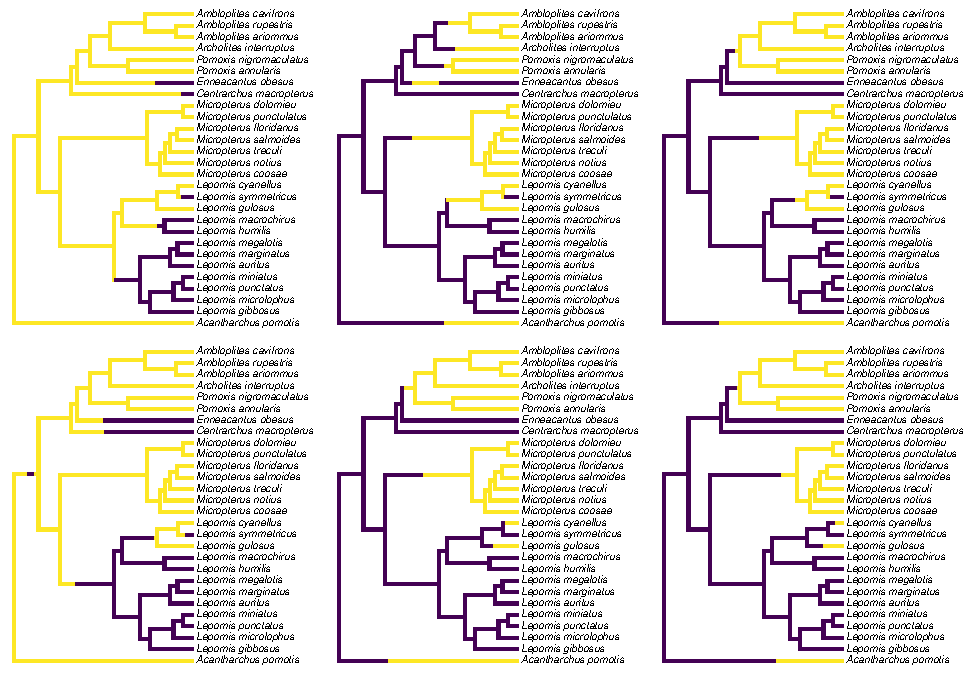
\includegraphics[width=1\linewidth]{old.Revell.phytools-v2_peerj_files/figure-latex/simmap-trees-1} %%%
\DIFdelendFL \DIFaddbeginFL 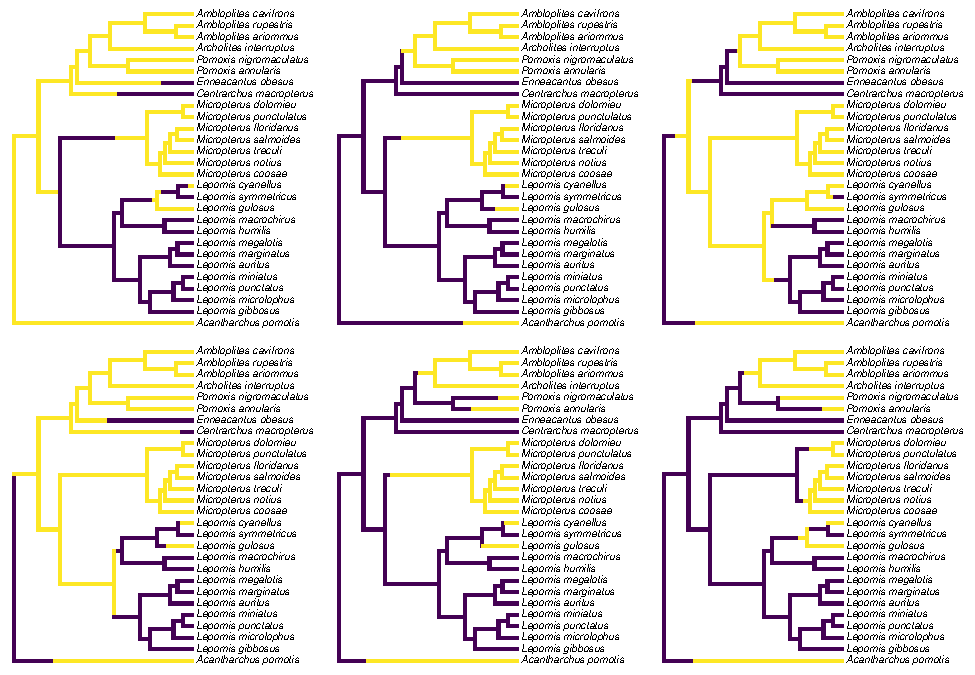
\includegraphics[width=1\linewidth]{Revell.phytools-v2_peerj_files/figure-latex/simmap-trees-1} \DIFaddendFL \caption{Six randomly chosen stochastic character maps of feeding mode (non-piscivorous, in dark blue, vs. piscivorous) on a phylogeny of 28 centrarchid fish species. Stochastic character mapping involves randomly sampling character histories that are consistent with our tip data in proportion to their probability under a model. In this case, histories were sampled under the set of four alternative M\textit{k} models of a binary trait, with relative frequencies proportional to the weight of evidence supporting each model. The tree and data are modified from Revell and Collar (2009). See main text for additional details.}\label{fig:simmap-trees}
\end{figure}

To create my color palette for plotting I used another contributed R
package that we haven't seen yet called \emph{viridisLite} by Garnier et
al. (2022). \DIFaddbegin \emph{\DIFadd{viridisLite}} \DIFadd{implements a color palette (known as the
``viridis'' palette and originally devised by van der Walt and Smith
2015) that was designed to be both attractive and colorblind-friendly.
}\DIFaddend To replicate Figure @ref(fig:simmap-trees) exactly, users should first
install \emph{viridisLite} from CRAN by running
\texttt{install.packages("viridisLite")} -- but they do not need to load
it. \DIFdelbegin \DIFdel{(}\DIFdelend Calling the contributed package function using the double colon
syntax, \texttt{::}, takes care of that \DIFdelbegin \DIFdel{-- }\DIFdelend \DIFaddbegin \DIFadd{(}\DIFaddend i.e.,
\texttt{viridisLite::viridis}\DIFdelbegin \DIFdel{.)}\DIFdelend \DIFaddbegin \DIFadd{).
}\DIFaddend 

Although Figure @ref(fig:simmap-trees) already gives us a general sense
of the uncertainty of our ancestral character history on the tree for
our trait, most commonly we don't want to simply graph a subset (or all)
of our stochastically mapped trees. Typically, instead, we'd first
summarize our stochastic character maps (in multiple ways), and then
proceed to plot or analyze these summarized findings.

\DIFdelbegin \DIFdel{Perhaps most often}\DIFdelend \DIFaddbegin \DIFadd{Often}\DIFaddend , \emph{phytools} users undertaking stochastic character mapping
will compute the posterior probabilities of each value of the character
trait at each internal node of the tree\DIFdelbegin \DIFdel{. }\DIFdelend \DIFaddbegin \DIFadd{, which one can obtain by simply
}\emph{\DIFadd{counting}} \DIFadd{the fraction of stochastic maps for which each node is
in each of the observed states of our character trait. These values
correspond to a form of ancestral state estimation, giving us an
approximation of the marginal probabilities that each hypothetical
ancestor at each node of the tree was in each of our observed states.
We've conditioned on our transition model and its Maximum Likelihood
parameter estimates -- although in this instance we also
}\emph{\DIFadd{integrate}} \DIFadd{across a set of four evolutionary models in proportion
to the weight of evidence in support of each one. }\DIFaddend In \emph{phytools},
these values \DIFaddbegin \DIFadd{marginal posterior probabilities }\DIFaddend can be obtained using the
generic \texttt{summary} method for our object class, which is then
easily plotted as follows.

\begin{Shaded}
\begin{Highlighting}[]
\FunctionTok{plot}\NormalTok{(}\FunctionTok{summary}\NormalTok{(sunfish.simmap),}\AttributeTok{ftype=}\StringTok{"i"}\NormalTok{,}\AttributeTok{fsize=}\FloatTok{0.7}\NormalTok{,}
  \AttributeTok{colors=}\NormalTok{cols,}\AttributeTok{cex=}\FunctionTok{c}\NormalTok{(}\FloatTok{0.6}\NormalTok{,}\FloatTok{0.3}\NormalTok{))}
\FunctionTok{legend}\NormalTok{(}\StringTok{"topleft"}\NormalTok{,}\FunctionTok{levels}\DIFdelbegin \DIFdel{\NormalTok{(feeding\_mode),}}\DIFdelend \DIFaddbegin \DIFadd{\NormalTok{(sunfish.feed\_mode),}}\DIFaddend \AttributeTok{pch=}\DecValTok{21}\NormalTok{,}
  \AttributeTok{pt.cex=}\FloatTok{1.5}\NormalTok{,}\AttributeTok{pt.bg=}\NormalTok{cols,}\AttributeTok{bty=}\StringTok{"n"}\NormalTok{,}\AttributeTok{cex=}\FloatTok{0.8}\NormalTok{)}
\end{Highlighting}
\end{Shaded}

\begin{figure}
\DIFdelbeginFL %DIFDELCMD < \includegraphics[width=1\linewidth]{old.Revell.phytools-v2_peerj_files/figure-latex/posterior-probs-1} %%%
\DIFdelendFL \DIFaddbeginFL \includegraphics[width=1\linewidth]{Revell.phytools-v2_peerj_files/figure-latex/posterior-probs-1} \DIFaddendFL \caption{Posterior probabilities at each ancestral node of the centrarchid tree of Figure 1 from stochastic character mapping using model weights to sample across four different extended M\textit{k} trait evolution models. See main text for more details.}\label{fig:posterior-probs}
\end{figure}

A correct interpretation of the graph of Figure
@ref(fig:posterior-probs) is that it shows the observed discrete
character states (at the tips of the tree) and the posterior
probabilities from stochastic mapping that each internal node is in each
state -- all while integrating over our four different transition models
in proportion to the weight of evidence \DIFdelbegin \DIFdel{in support of }\DIFdelend \DIFaddbegin \DIFadd{for }\DIFaddend each model!

In addition to node probabilities, \emph{phytools} users undertaking a
stochastic character mapping analysis are often interested in the number
of changes of each type that are implied by the evolutionary process and
our data. The procedure of stochastic mapping samples full character
histories (not just states or probabilities at nodes) \DIFdelbegin \DIFdel{, }\DIFdelend and can thus be
deployed to produce estimates of the posterior probability distribution
of the character changes of each type on specific edges, in specific
clades, or \DIFdelbegin \DIFdel{on the entire tree}\DIFdelend \DIFaddbegin \DIFadd{across the entire phylogeny}\DIFaddend , conditioning on our sampled
model or models.

To obtain these distributions, we'll first call the generic method
\texttt{density} which (when \DIFdelbegin \DIFdel{given }\DIFdelend \DIFaddbegin \DIFadd{applied to }\DIFaddend an object from stochastic
mapping) computes the relative frequency distribution of changes of each
type over the whole tree. We can then \DIFdelbegin \DIFdel{graph these distributions (remember, }\DIFdelend \DIFaddbegin \DIFadd{proceed to graph our results using
a different generic }\texttt{\DIFadd{plot}} \DIFadd{method, as follows. Remember, }\DIFaddend our
character is binary, so there are only two types of character state
\DIFdelbegin \DIFdel{change: }\DIFdelend \DIFaddbegin \DIFadd{changes: from }\DIFaddend non-piscivorous \(\rightarrow\) piscivorous, and the
reverse\DIFdelbegin \DIFdel{)
using a different generic }\texttt{\DIFdel{plot}} %DIFAUXCMD
\DIFdel{method, as follows}\DIFdelend .

\begin{Shaded}
\begin{Highlighting}[]
\NormalTok{sunfish.density}\OtherTok{\textless{}{-}}\FunctionTok{density}\NormalTok{(sunfish.simmap)}
\NormalTok{sunfish.density}
\end{Highlighting}
\end{Shaded}

\begin{verbatim}
## 
## Distribution of changes from stochastic mapping:
##  non-piscivorous->piscivorous        piscivorous->non-piscivorous
##  Min.   :0   Min.   :0
##  Median :5   Median :2
##  Mean   :4.13    Mean   :2.24
##  Max.   :10  Max.   :9
## 
## 95% HPD interval(non-piscivorous->piscivorous): [0, 8]
## 95% HPD interval(piscivorous->non-piscivorous): [0, 6]
\end{verbatim}

\begin{Shaded}
\begin{Highlighting}[]
\FunctionTok{par}\NormalTok{(}\AttributeTok{mfrow=}\FunctionTok{c}\NormalTok{(}\DecValTok{1}\NormalTok{,}\DecValTok{2}\NormalTok{),}\AttributeTok{las=}\DecValTok{1}\NormalTok{,}\AttributeTok{cex.axis=}\FloatTok{0.7}\NormalTok{,}\AttributeTok{cex.lab=}\FloatTok{0.8}\NormalTok{)}
\NormalTok{COLS}\OtherTok{\textless{}{-}}\FunctionTok{setNames}\NormalTok{(cols[}\DecValTok{2}\SpecialCharTok{:}\DecValTok{1}\NormalTok{],sunfish.density}\SpecialCharTok{$}\NormalTok{trans)}
\FunctionTok{plot}\NormalTok{(sunfish.density,}\AttributeTok{ylim=}\FunctionTok{c}\NormalTok{(}\DecValTok{0}\NormalTok{,}\FloatTok{0.6}\NormalTok{),}
  \AttributeTok{transition=}\FunctionTok{names}\NormalTok{(COLS)[}\DecValTok{1}\NormalTok{],}\AttributeTok{colors=}\NormalTok{COLS[}\DecValTok{1}\NormalTok{],}\AttributeTok{main=}\StringTok{""}\NormalTok{)}
\FunctionTok{mtext}\NormalTok{(}\StringTok{"a) transitions to piscivory"}\NormalTok{,}\AttributeTok{line=}\DecValTok{1}\NormalTok{,}\AttributeTok{adj=}\DecValTok{0}\NormalTok{,}
  \AttributeTok{cex=}\FloatTok{0.8}\NormalTok{)}
\FunctionTok{plot}\NormalTok{(sunfish.density,}\AttributeTok{ylim=}\FunctionTok{c}\NormalTok{(}\DecValTok{0}\NormalTok{,}\FloatTok{0.6}\NormalTok{),}
  \AttributeTok{transition=}\FunctionTok{names}\NormalTok{(COLS)[}\DecValTok{2}\NormalTok{],}\AttributeTok{colors=}\NormalTok{COLS[}\DecValTok{2}\NormalTok{],}\AttributeTok{main=}\StringTok{""}\NormalTok{)}
\FunctionTok{mtext}\NormalTok{(}\StringTok{"b) transitions to non{-}piscivory"}\NormalTok{,}\AttributeTok{line=}\DecValTok{1}\NormalTok{,}\AttributeTok{adj=}\DecValTok{0}\NormalTok{,}
  \AttributeTok{cex=}\FloatTok{0.8}\NormalTok{)}
\end{Highlighting}
\end{Shaded}

\begin{figure}
\DIFdelbeginFL %DIFDELCMD < \includegraphics[width=1\linewidth]{old.Revell.phytools-v2_peerj_files/figure-latex/num-changes-1} %%%
\DIFdelendFL \DIFaddbeginFL \includegraphics[width=1\linewidth]{Revell.phytools-v2_peerj_files/figure-latex/num-changes-1} \DIFaddendFL \caption{Posterior probability distributions of changes from either a) non-piscivory to piscivory, or b) piscivory to non-piscivory, obtained from an analysis of stochastic mapping. HPD indicates the 95\% high probability density interval for changes of each type. See main text for additional details.}\label{fig:num-changes}
\end{figure}

The distributions shown in Figure @ref(fig:num-changes) give the
relative frequencies of changes of each type across our set of mapped
histories, as well as Bayesian 95\% high probability density (HPD)
intervals calculated using the R pakage \emph{coda} (Plummer et al.
2006). \DIFaddbegin \DIFadd{For a binary trait like that of this example (and thus with only
two types of transitions), we could have instead overlain the
distributions of backwards and forwards transitions in character state
in a single plot panel. In this particular instance, however, I found
that overplotting the two different distributions resulted in a figure
that was too difficult to read, and preferred instead to show the
distributions in separate panels as in Figure @ref(fig:num-changes). For
multistate characters with more than two types of changes between
states, the same }\texttt{\DIFadd{plot}} \DIFadd{method will produce a }\emph{\DIFadd{k}} \DIFadd{\(\times\)
}\emph{\DIFadd{k}} \DIFadd{matrix of figure panels, each }\emph{\DIFadd{i}}\DIFadd{,}\emph{\DIFadd{j}}\DIFadd{th panel of
which will contain the posterior distribution of changes from character
state }\emph{\DIFadd{i}} \DIFadd{to }\emph{\DIFadd{j}}\DIFadd{.
}\DIFaddend 

An interesting attribute of the character state change distributions for
\DIFdelbegin \DIFdel{our }\DIFdelend \DIFaddbegin \DIFadd{this }\DIFaddend centrarchid feeding mode \DIFdelbegin \DIFdel{data }\DIFdelend \DIFaddbegin \DIFadd{analysis }\DIFaddend is that they are both markedly
bi-modal. This is due, in part, to our specific procedure of
model-averaging in which we sampled both reversible and irreversible
character evolution models in proportion to their weights, and isn't
something we would've seen had we chosen to analyze just one model or
the other. (Recall that the weight of evidence was highly similar
between our equal-rates model and the irreversible model in which
piscivory is acquired from non-piscivory, but never the reverse. \DIFdelbegin \DIFdel{)
}\DIFdelend \DIFaddbegin \DIFadd{See
above.) This pattern is also appropriately captured by the broad HPD
intervals on each of the two types of transitions.
}\DIFaddend 

Lastly, in addition to these analyses, \emph{phytools} also makes it
quite straightforward to visualize the posterior probabilities of each
of the two trait conditions not only at nodes, but also also along the
branches of the phylogeny. This is accomplished using the
\emph{phytools} function \texttt{densityMap} (Revell 2013), which
creates a graph showing the probability density of stochastic histories
in each of our mapped states. By design, in \emph{phytools} this object
can be first created (using the \texttt{densityMap} function), updated
(using the method \texttt{setMap} to adjust our color palette for
plotting), and then graphed (using a generic \texttt{plot} method that
was created for this specific object class). \DIFaddbegin \DIFadd{I'll illustrate this set of
procedures in the following code block.
}\DIFaddend 

\begin{Shaded}
\begin{Highlighting}[]
\NormalTok{sunfish.densityMap}\OtherTok{\textless{}{-}}\FunctionTok{densityMap}\NormalTok{(sunfish.simmap,}\AttributeTok{plot=}\ConstantTok{FALSE}\NormalTok{,}
  \AttributeTok{res=}\DecValTok{1000}\NormalTok{)}
\NormalTok{sunfish.densityMap}
\end{Highlighting}
\end{Shaded}

\begin{verbatim}
## Object of class "densityMap" containing:
## 
## (1) A phylogenetic tree with 28 tips and 27 internal nodes.
## 
## (2) The mapped posterior density of a discrete binary character
##     with states (non-piscivorous, piscivorous).
\end{verbatim}

\begin{Shaded}
\begin{Highlighting}[]
\NormalTok{sunfish.densityMap}\OtherTok{\textless{}{-}}\FunctionTok{setMap}\NormalTok{(sunfish.densityMap,}
\NormalTok{  viridisLite}\SpecialCharTok{::}\FunctionTok{viridis}\NormalTok{(}\AttributeTok{n=}\DecValTok{10}\NormalTok{))}
\FunctionTok{plot}\NormalTok{(sunfish.densityMap,}\AttributeTok{lwd=}\DecValTok{3}\NormalTok{,}\AttributeTok{outline=}\ConstantTok{TRUE}\NormalTok{,}
  \AttributeTok{fsize=}\DIFdelbegin \DIFdel{\FloatTok{0.7}\NormalTok{,}}\DIFdelend \DIFaddbegin \DIFadd{\FunctionTok{c}\NormalTok{(}\FloatTok{0.6}\NormalTok{,}\FloatTok{0.7}\NormalTok{),}}\DIFaddend \AttributeTok{legend=}\FloatTok{0.1}\NormalTok{)}
\end{Highlighting}
\end{Shaded}

\begin{figure}
\DIFdelbeginFL %DIFDELCMD < 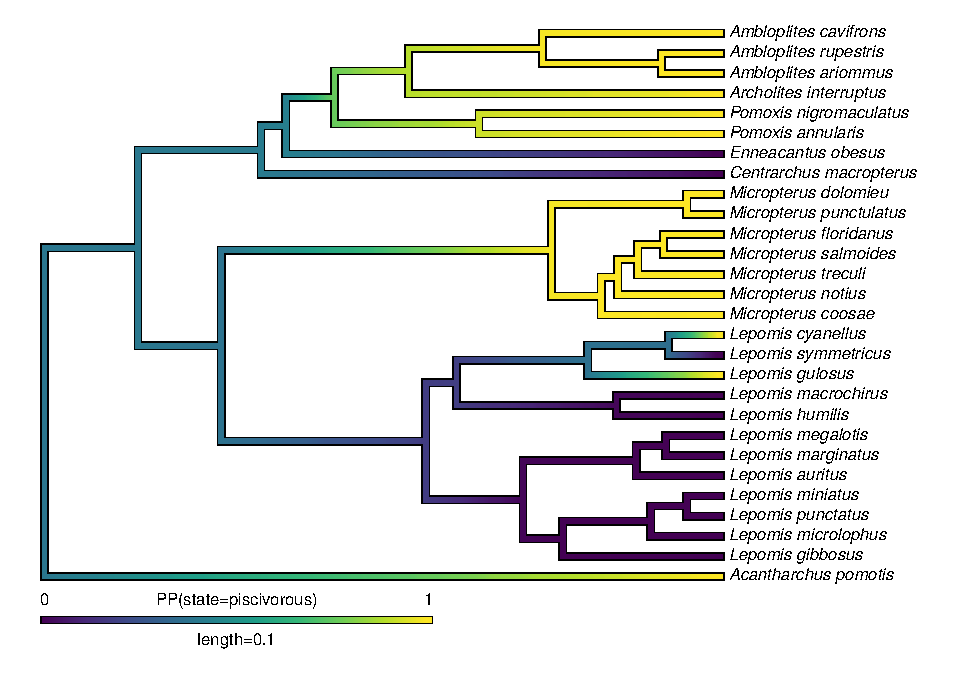
\includegraphics[width=1\linewidth]{old.Revell.phytools-v2_peerj_files/figure-latex/densityMap-1} %%%
\DIFdelendFL \DIFaddbeginFL 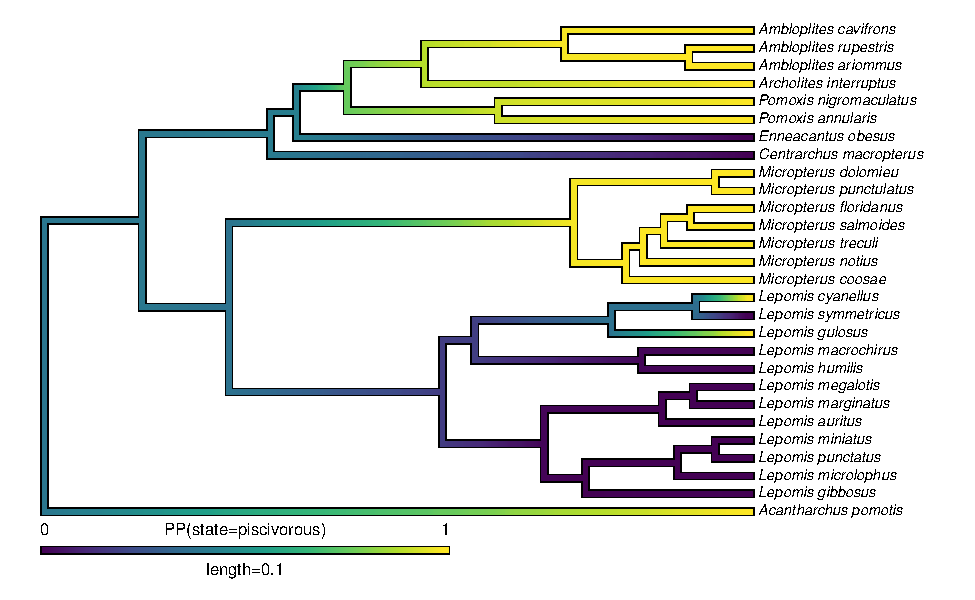
\includegraphics[width=1\linewidth]{Revell.phytools-v2_peerj_files/figure-latex/densityMap-1} \DIFaddendFL \caption{Posterior probability density of each of the two character levels, piscivory and non-piscivory, \DIFdelbeginFL \DIFdelFL{mapped }\DIFdelendFL \DIFaddbeginFL \DIFaddFL{based on stochastic character mapping, graphed }\DIFaddendFL along the edges of a tree of centrarchid fishes \DIFaddbeginFL \DIFaddFL{using a color gradient}\DIFaddendFL . See main text for more details.}\label{fig:densityMap}
\end{figure}

\DIFaddbegin \DIFadd{Having enthusiastically demonstrated the model-averaging feature of the
new }\emph{\DIFadd{phytools}} \texttt{\DIFadd{simmap}} \DIFadd{method, I'd be remiss if I failed to
note that this is }\emph{\DIFadd{not}} \DIFadd{(as yet) the standard workflow for
ancestral state reconstruction of discrete characters in general, nor
for stochastic mapping in particular. More typically, researchers select
the best model and then proceed to hold this model (and its parameters)
constant through subsequent calculations (e.g., Yang 2014), }\emph{\DIFadd{or}}
\DIFadd{they sample parameter values for a single model from their joint
posterior distribution using MCMC (e.g., shown in Revell and Harmon
2022). I think, however, that there is a very strong case to be made
that if, for example, 51\% of the weight of evidence points to a model
in which a specific node has a high conditional probability of being in
state }\emph{\DIFadd{a}}\DIFadd{, while 49\% of the weight of evidence points to a model
wherein the same node has a high probability of being in state }\emph{\DIFadd{b}}\DIFadd{,
then the correct marginal probability that the node is }\emph{\DIFadd{actually}}
\DIFadd{in state }\emph{\DIFadd{a}} \DIFadd{is probably closer to 0.5 than 1.0. Indeed, this would
be our exact interpretation of this result if we consider the model
weights as the probability that each model is correct (assuming that all
possible models are in our set, e.g., Link and Barker 2006).
}

\DIFadd{Apart from the analyses shown, stochastic mapping as implemented in
}\emph{\DIFadd{phytools}} \DIFadd{is a very flexible method via which we might sample the
matrix of transition rates from its posterior distribution under a
model, incorporate uncertainty in the character state values for
different species, take into account polymorphic character conditions
and hidden-rates of trait evolution, and integrate over phylogenetic
uncertainty. A comprehensive survey of this functionality is beyond the
scope of the present article; however, considerable additional
information about stochastic mapping in R can be found in the
}\emph{\DIFadd{phytools}} \DIFadd{documentation pages as well as elsewhere online.
}

\DIFaddend \hypertarget{the-polymorphic-trait-evolution-model}{%
\subsection{The polymorphic trait evolution
model}\label{the-polymorphic-trait-evolution-model}}

Another important, but much more recently-added, tool in the
\emph{phytools} R package is a method (called \texttt{fitpolyMk}) that's
designed to fit a discrete character evolution model to trait data
containing intraspecific polymorphism (Revell and Harmon 2022). In this
case, our model is one in which an evolutionary transition from (say)
character state \emph{a} to character state \emph{b} must first pass
through the intermediate polymorphic condition of \emph{a} + \emph{b}.
This model starts off very simply -- but will become increasingly
complicated for increasing numbers of monomorphic conditions of our
trait. Not only that, but as soon as we have more than two monomorphic
states, we must also consider whether our character is evolving in an
ordered (Figure @ref(fig:structure-polyMk)a) or unordered (Figure
@ref(fig:structure-polyMk)b) fashion (Revell and Harmon 2022). \DIFdelbegin %DIFDELCMD < 

%DIFDELCMD < %%%
\DIFdelend Figure
@ref(fig:structure-polyMk) shows the general structure of an ordered and
unordered polymorphic trait evolution model -- both for the same\DIFaddbegin \DIFadd{,
underlying }\DIFaddend number of monomorphic conditions of our trait (four).

\begin{Shaded}
\begin{Highlighting}[]
\FunctionTok{par}\NormalTok{(}\AttributeTok{mfrow=}\FunctionTok{c}\NormalTok{(}\DecValTok{1}\NormalTok{,}\DecValTok{2}\NormalTok{))}
\FunctionTok{graph.polyMk}\NormalTok{(}\AttributeTok{k=}\DecValTok{4}\NormalTok{,}\AttributeTok{ordered=}\ConstantTok{TRUE}\NormalTok{,}\AttributeTok{states=}\DecValTok{0}\SpecialCharTok{:}\DecValTok{3}\NormalTok{,}
  \AttributeTok{mar=}\FunctionTok{rep}\NormalTok{(}\FloatTok{0.1}\NormalTok{,}\DecValTok{4}\NormalTok{))}
\FunctionTok{mtext}\NormalTok{(}\StringTok{"a) ordered polymorphic model"}\NormalTok{,}\AttributeTok{line=}\SpecialCharTok{{-}}\DecValTok{1}\NormalTok{,}\AttributeTok{adj=}\FloatTok{0.2}\NormalTok{,}
  \AttributeTok{cex=}\FloatTok{0.8}\NormalTok{)}
\FunctionTok{graph.polyMk}\NormalTok{(}\AttributeTok{k=}\DecValTok{4}\NormalTok{,}\AttributeTok{ordered=}\ConstantTok{FALSE}\NormalTok{,}\AttributeTok{states=}\NormalTok{letters[}\DecValTok{1}\SpecialCharTok{:}\DecValTok{4}\NormalTok{],}
  \AttributeTok{mar=}\FunctionTok{rep}\NormalTok{(}\FloatTok{0.1}\NormalTok{,}\DecValTok{4}\NormalTok{),}\AttributeTok{spacer=}\FloatTok{0.15}\NormalTok{)}
\FunctionTok{mtext}\NormalTok{(}\StringTok{"b) unordered polymorphic model"}\NormalTok{,}\AttributeTok{line=}\SpecialCharTok{{-}}\DecValTok{1}\NormalTok{,}
  \AttributeTok{adj=}\FloatTok{0.2}\NormalTok{,}\AttributeTok{cex=}\FloatTok{0.8}\NormalTok{)}
\end{Highlighting}
\end{Shaded}

\begin{figure}
\DIFdelbeginFL %DIFDELCMD < \includegraphics[width=1\linewidth]{old.Revell.phytools-v2_peerj_files/figure-latex/structure-polyMk-1} %%%
\DIFdelendFL \DIFaddbeginFL \includegraphics[width=1\linewidth]{Revell.phytools-v2_peerj_files/figure-latex/structure-polyMk-1} \DIFaddendFL \caption{Example structures of two alternative polymorphic trait evolution models for characters with four monomorphic conditions: a) an ordered model with states 0 to 3; b) an unordered model, with states \textit{a}, \textit{b}, \textit{c}, and \textit{d}. \DIFaddbeginFL \DIFaddFL{The maximum parameter complexity of each model corresponds to 2 $\times$ the number of double-ended arrows in the panel. }\DIFaddendFL See main text for additional details.}\label{fig:structure-polyMk}
\end{figure}

Obviously, the potential parameter complexity of the unordered
polymorphic trait evolution model is higher than the ordered model.
Since there exists an unordered model that also has all ordered models
as a special case, ordered and unordered models can be compared using
likelihood-ratio tests (if nested) or information criteria.

To try out our polymorphic trait evolution model, let's use an
excellent, recently-published dataset from Halali et al. (2020)
consisting of a phylogenetic tree containing 287 Mycalesina butterfly
species and data for butterfly habitat use. Halali et al. (2020) coded
habitat as a polymorphic trait in which, for example, a species using
both ``forest'' and forest ``fringe'' habitat would be \DIFdelbegin \DIFdel{coded }\DIFdelend \DIFaddbegin \DIFadd{recorded }\DIFaddend as
\texttt{"forest+fringe"}. In this case, our polymorphic trait evolution
model will assume that to evolve from forest specialization to fringe
specialization, a species must first (at least transiently) evolve
through the polymorphic condition of using both habitats at once. This
seems logical.

The Halali et al. (2020) dataset and tree now come packaged with the
\emph{phytools} library, so both can be loaded using the \texttt{data}
function, just as we \DIFdelbegin \DIFdel{'ve seen already for other datasets of this article}\DIFdelend \DIFaddbegin \DIFadd{saw for the centrarchid data and tree of our
previous example}\DIFaddend .

\begin{Shaded}
\begin{Highlighting}[]
\FunctionTok{data}\NormalTok{(butterfly.tree)}
\FunctionTok{data}\NormalTok{(butterfly.data)}
\end{Highlighting}
\end{Shaded}

Let's begin by inspecting our data.

\begin{Shaded}
\begin{Highlighting}[]
\FunctionTok{head}\NormalTok{(butterfly.data)}
\end{Highlighting}
\end{Shaded}

\begin{verbatim}
##                                     habitat
## Myc_francisca_formosana? forest+fringe+open
## Bic_cooksoni                           open
## Bic_brunnea                          forest
## Bic_jefferyi                    fringe+open
## Bic_auricruda_fulgida                forest
## Bic_smithi_smithi             forest+fringe
\end{verbatim}

\texttt{fitpolyMk} requires us to separate the different states in each
polymorphic condition using the \texttt{+} symbol, but does not demand
that our states be ordered in a consistent manner. In other words,
\texttt{a+b} and \texttt{b+a} would be considered (properly) to be same
polymorphic condition! \DIFdelbegin %DIFDELCMD < 

%DIFDELCMD < %%%
\DIFdelend As a first preliminary step in our analysis, we
can proceed to extract the column of habitat use data (\texttt{habitat}
in our data frame) as a vector, and then print the different levels that
it takes.

\begin{Shaded}
\begin{Highlighting}[]
\NormalTok{butterfly.habitat}\OtherTok{\textless{}{-}}\FunctionTok{setNames}\DIFdelbegin \DIFdel{\NormalTok{(}
\NormalTok{  butterfly.data}}\DIFdelend \DIFaddbegin \DIFadd{\NormalTok{(butterfly.data}}\DIFaddend \SpecialCharTok{$}\NormalTok{habitat,}
  \FunctionTok{rownames}\NormalTok{(butterfly.data))}
\FunctionTok{print}\NormalTok{(}\FunctionTok{levels}\NormalTok{(butterfly.habitat))}
\end{Highlighting}
\end{Shaded}

\begin{verbatim}
## [1] "forest"             "forest+fringe"      "forest+fringe+open" "fringe"             "fringe+open"       
## [6] "open"
\end{verbatim}

Now, let's proceed to fit our polymorphic trait evolution model to these
data. \DIFdelbegin %DIFDELCMD < 

%DIFDELCMD < %%%
\DIFdelend In this instance, I'll fit a grand total of six different models.
\DIFdelbegin \DIFdel{(}\DIFdelend This isn't a comprehensive set of the conceivable models for polymorphic
data with these levels, but it seemed like a reasonable selection for
illustrative purposes.
\DIFdelbegin \DIFdel{)
}\DIFdelend 

The first three of these models all suppose that the evolution of my
discrete character is totally unordered. Among this set, we'll imagine,
first, equal transition rates between all monomorphic states or
polymorphic conditions. For our second model, we'll permit all possible
transition rates between states or state combinations to assume
\DIFdelbegin \DIFdel{different }\DIFdelend \DIFaddbegin \emph{\DIFadd{different}} \DIFaddend values. Finally, for our third model we'll assume that
the acquisition of polymorphism (or its increase) occurs with one rate,
whereas the loss (or decrease) of polymorphism occurs with another,
separate rate. \DIFdelbegin %DIFDELCMD < 

%DIFDELCMD < %%%
\DIFdelend We refer to this last scenario as the ``transient model''
following Revell and Harmon (2022). \DIFdelbegin \DIFdel{The name for this }\DIFdelend \DIFaddbegin \DIFadd{This name for the }\DIFaddend model comes from
the general notion that if the rate of loss exceeds the rate of gain,
then polymorphism will typically be relatively transient in nature.
Since polymorphism tends to be less frequently observed in the types of
data that typify many phylogenetic comparative studies, including this
model in our set seems like a reasonable idea.

To get our remaining three models, and reach the six total models that I
promised at the outset of this section -- for each of the three listed
above in which character evolution is unordered, we'll simply add a
second \emph{ordered} model in which we assume that character evolution
for our three monomorphic conditions tends to proceed as follows:
\emph{forest} \(\leftrightarrow\) \emph{fringe} \(\leftrightarrow\)
\emph{open} -- not forgetting, of course, about the intermediate
polymorphic conditions \DIFdelbegin \DIFdel{that occur in between each of these }\DIFdelend \DIFaddbegin \DIFadd{found between each pair of }\DIFaddend monomorphic states!

To fit our first three models in R, we'll use the function
\texttt{fitpolyMk} from the \emph{phytools} package as follows.

\begin{Shaded}
\begin{Highlighting}[]
\NormalTok{butterfly.ER\_unordered}\OtherTok{\textless{}{-}}\FunctionTok{fitpolyMk}\DIFdelbegin \DIFdel{\NormalTok{(}
\NormalTok{  butterfly.tree,butterfly.habitat,}
  }\DIFdelend \DIFaddbegin \DIFadd{\NormalTok{(butterfly.tree,}
\NormalTok{  butterfly.habitat,}}\DIFaddend \AttributeTok{model=}\StringTok{"ER"}\NormalTok{)}
\end{Highlighting}
\end{Shaded}

\begin{verbatim}
## 
## This is the design matrix of the fitted model.
## Does it make sense?
## 
##                    forest fringe open
## forest                  0      0    0
## fringe                  0      0    0
## open                    0      0    0 
## forest+fringe           1      1    0
## forest+open             1      0    1
## fringe+open             0      1    1
## forest+fringe+open      0      0    0
##                    forest+fringe forest+open fringe+open
## forest                         1           1           0
## fringe                         1           0           1
## open                           0           1           1
## forest+fringe                  0           0           0
## forest+open                    0           0           0
## fringe+open                    0           0           0
## forest+fringe+open             1           1           1
##                    forest+fringe+open
## forest                              0
## fringe                              0
## open                                0
## forest+fringe                       1
## forest+open                         1
## fringe+open                         1
## forest+fringe+open                  0
\end{verbatim}

By default, \texttt{fitpolyMk} \DIFdelbegin \DIFdel{prints }\DIFdelend \DIFaddbegin \DIFadd{begins by printing }\DIFaddend out the design matrix
of the model for us to verify. \DIFdelbegin \DIFdel{(}\DIFdelend The design matrix is of dimensions
dictated by the number of states and polymorphic conditions of our
character, with integers populating the different types of transitions,
from row to column, that should be permitted under our model \DIFdelbegin \DIFdel{, }\DIFdelend \DIFaddbegin \DIFadd{-- }\DIFaddend and
zeros indicating \DIFdelbegin \DIFdel{unallowed }\DIFdelend \DIFaddbegin \DIFadd{disallowed }\DIFaddend transition types. The specific integer
values don't mean anything; however, different integer values imply that
the corresponding transitions will be allowed to take place with
different rates under our model.
\DIFdelbegin \DIFdel{)
}\DIFdelend 

This can be helpful, because we should find that it corresponds with the
design matrix that was discussed under the simpler M\emph{k} model of
the previous section -- as well as with the graphed models of Figure
@ref(fig:structure-polyMk). If we don't want the design matrix to print,
though, we can turn off this behavior simply by setting the optional
argument \texttt{quiet=TRUE}. \DIFdelbegin %DIFDELCMD < 

%DIFDELCMD < %%%
\DIFdelend Let's do that for our remaining two
unordered models.

\begin{Shaded}
\begin{Highlighting}[]
\NormalTok{butterfly.ARD\_unordered}\OtherTok{\textless{}{-}}\FunctionTok{fitpolyMk}\DIFdelbegin \DIFdel{\NormalTok{(}
\NormalTok{  butterfly.tree,butterfly.habitat,}
  }\DIFdelend \DIFaddbegin \DIFadd{\NormalTok{(butterfly.tree,}
\NormalTok{  butterfly.habitat,}}\DIFaddend \AttributeTok{model=}\StringTok{"ARD"}\NormalTok{,}\AttributeTok{quiet=}\ConstantTok{TRUE}\NormalTok{,}
  \AttributeTok{opt.method=}\StringTok{"optimParallel"}\NormalTok{,}\AttributeTok{rand\_start=}\ConstantTok{TRUE}\NormalTok{)}
\NormalTok{butterfly.transient\_unordered}\OtherTok{\textless{}{-}}\FunctionTok{fitpolyMk}\NormalTok{(}
\NormalTok{  butterfly.tree,butterfly.habitat,}
  \AttributeTok{model=}\StringTok{"transient"}\NormalTok{,}\AttributeTok{quiet=}\ConstantTok{TRUE}\NormalTok{,}
  \AttributeTok{opt.method=}\StringTok{"optimParallel"}\NormalTok{,}\AttributeTok{rand\_start=}\ConstantTok{TRUE}\NormalTok{)}
\end{Highlighting}
\end{Shaded}

Astute readers may notice that I added two additional arguments that
didn't feature in my previous \texttt{fitpolyMk} function call:
\texttt{opt.method="optimParallel"} and \texttt{rand\_start=TRUE}. The
former tells my optimizer to use the \emph{optimParallel} package
(Gerber and Furrer 2019) for optimization. The latter says ``choose
random starting values.'' Both of these, and sometimes multiple
optimization replicates, may be required to find our Maximum Likelihood
solution for these complex models. \DIFdelbegin \DIFdel{(}\DIFdelend In fact, I virtually guarantee it!
\DIFdelbegin \DIFdel{)
}\DIFdelend 

\DIFdelbegin \DIFdel{We're not done fitting models yet, but to see how things are going so
far, why don't we compare our three fitted models using the generic
}\texttt{\DIFdel{anova}} %DIFAUXCMD
\DIFdel{method of their object class, as follows.
}%DIFDELCMD < 

%DIFDELCMD < \begin{Shaded}
%DIFDELCMD < \begin{Highlighting}[]
%DIFDELCMD < %%%
\DIFdel{\FunctionTok{anova}\NormalTok{(butterfly.ER\_unordered,}
\NormalTok{  butterfly.ARD\_unordered,}
\NormalTok{  butterfly.transient\_unordered)}
}%DIFDELCMD < \end{Highlighting}
%DIFDELCMD < \end{Shaded}
%DIFDELCMD < 

%DIFDELCMD < \begin{verbatim}
%DIFDELCMD < %%%
%DIFAUXCMD NEXT
\DIFmodbegin
\begin{DIFverbatim}[alsolanguage=DIFcode]
%DIF < ##                                  log(L) d.f.      AIC       weight
%DIF < ## object                        -355.8122    1 713.6244 1.017751e-19
%DIF < ## butterfly.ARD_unordered       -295.0807   18 626.1614 1.000000e+00
%DIF < ## butterfly.transient_unordered -353.4496    2 710.8991 3.975914e-19
\end{DIFverbatim}
\DIFmodend %DIFAUXCMD
%DIFDELCMD < \end{verbatim}
%DIFDELCMD < 

%DIFDELCMD < %%%
\DIFdel{This tells us that, just among the three models that we've considered to
this point in our analysis, the best-supported by a wide margin is our
parameter-rich all-rates-different (}\texttt{\DIFdel{"ARD"}}%DIFAUXCMD
\DIFdel{) model.
}%DIFDELCMD < 

%DIFDELCMD < %%%
\DIFdelend Now we can proceed to do the same thing, but this time updating the
argument value \texttt{ordered} to \texttt{ordered=TRUE}\DIFdelbegin \DIFdel{; however, when
}\DIFdelend \DIFaddbegin \DIFadd{. When }\DIFaddend we switch
from fitting an unordered polymorphic trait evolution model to our
ordered model, it suddenly becomes critical that we specify the order
levels using the optional function argument \texttt{order}. If
\texttt{order} isn't indicated, \texttt{fitpolyMk} will simply assume
that our characters are ordered alphanumerically -- but this is very
rarely likely to be correct! (By chance, it happens to be true of our
butterfly dataset. I assigned the argument \texttt{order} anyway, just
to be safe\DIFdelbegin \DIFdel{!}\DIFdelend \DIFaddbegin \DIFadd{.}\DIFaddend )

\begin{Shaded}
\begin{Highlighting}[]
\NormalTok{levs}\OtherTok{\textless{}{-}}\FunctionTok{c}\NormalTok{(}\StringTok{"forest"}\NormalTok{,}\StringTok{"fringe"}\NormalTok{,}\StringTok{"open"}\NormalTok{)}
\NormalTok{levs}
\end{Highlighting}
\end{Shaded}

\begin{verbatim}
## [1] "forest" "fringe" "open"
\end{verbatim}

\begin{Shaded}
\begin{Highlighting}[]
\NormalTok{butterfly.ER\_ordered}\OtherTok{\textless{}{-}}\FunctionTok{fitpolyMk}\DIFdelbegin \DIFdel{\NormalTok{(}
\NormalTok{  butterfly.tree,butterfly.habitat,}
  }\DIFdelend \DIFaddbegin \DIFadd{\NormalTok{(butterfly.tree,}
\NormalTok{  butterfly.habitat,}}\DIFaddend \AttributeTok{model=}\StringTok{"ER"}\NormalTok{,}\AttributeTok{ordered=}\ConstantTok{TRUE}\NormalTok{,}\AttributeTok{order=}\NormalTok{levs,}
  \AttributeTok{quiet=}\ConstantTok{TRUE}\NormalTok{)}
\NormalTok{butterfly.ARD\_ordered}\OtherTok{\textless{}{-}}\FunctionTok{fitpolyMk}\DIFdelbegin \DIFdel{\NormalTok{(}
\NormalTok{  butterfly.tree,butterfly.habitat,}
  }\DIFdelend \DIFaddbegin \DIFadd{\NormalTok{(butterfly.tree,}
\NormalTok{  butterfly.habitat,}}\DIFaddend \AttributeTok{model=}\StringTok{"ARD"}\NormalTok{,}\AttributeTok{ordered=}\ConstantTok{TRUE}\NormalTok{,}
  \AttributeTok{order=}\NormalTok{levs,}\AttributeTok{quiet=}\ConstantTok{TRUE}\NormalTok{,}\AttributeTok{opt.method=}\StringTok{"optimParallel"}\NormalTok{,}
  \AttributeTok{rand\_start=}\ConstantTok{TRUE}\NormalTok{)}
\NormalTok{butterfly.transient\_ordered}\OtherTok{\textless{}{-}}\FunctionTok{fitpolyMk}\DIFdelbegin \DIFdel{\NormalTok{(}
\NormalTok{  butterfly.tree,butterfly.habitat,}
  }\DIFdelend \DIFaddbegin \DIFadd{\NormalTok{(butterfly.tree,}
\NormalTok{  butterfly.habitat,}}\DIFaddend \AttributeTok{model=}\StringTok{"transient"}\NormalTok{,}\AttributeTok{ordered=}\ConstantTok{TRUE}\NormalTok{,}
  \AttributeTok{order=}\NormalTok{levs,}\AttributeTok{quiet=}\ConstantTok{TRUE}\NormalTok{,}\AttributeTok{opt.method=}\StringTok{"optimParallel"}\NormalTok{,}
  \AttributeTok{rand\_start=}\ConstantTok{TRUE}\NormalTok{)}
\end{Highlighting}
\end{Shaded}

Now, with all six models in hand, let's compare them using \DIFdelbegin \DIFdel{a second
}\DIFdelend \DIFaddbegin \DIFadd{an
}\DIFaddend \texttt{anova} call as follows. \DIFdelbegin \DIFdel{This time }\DIFdelend I'll save my results from our model
comparison to the object \texttt{butterfly.aov}.

\begin{Shaded}
\begin{Highlighting}[]
\NormalTok{butterfly.aov}\OtherTok{\textless{}{-}}\FunctionTok{anova}\NormalTok{(butterfly.ER\_ordered,}
\NormalTok{  butterfly.ER\_unordered,}
\NormalTok{  butterfly.transient\_ordered,}
\NormalTok{  butterfly.transient\_unordered,}
\NormalTok{  butterfly.ARD\_ordered,}
\NormalTok{  butterfly.ARD\_unordered)}
\end{Highlighting}
\end{Shaded}

\begin{verbatim}
##                                  log(L) d.f.      AIC       weight
## object                        -329.0390    1 660.0779 1.472873e-09
## butterfly.ER_unordered        -355.8122    1 713.6244 3.472845e-21
## butterfly.transient_ordered   -329.0205    2 662.0409 5.519508e-10
## butterfly.transient_unordered -353.4496    2 710.8991 1.356691e-20
## butterfly.ARD_ordered         -297.7376   12 619.4753 9.658773e-01
## butterfly.ARD_unordered       -295.0807   18 626.1614 3.412273e-02
\end{verbatim}

A quick word of caution to readers is probably merited \DIFaddbegin \DIFadd{here}\DIFaddend . These
models can be quite difficult to optimize, meaning that it's not
inconceivable to imagine that (in spite of our best efforts)
\texttt{fitpolyMk} hasn't converged on the true Maximum Likelihood
solution for one model or another. Although the true best solution may
be unknowable (this is why we use numerical optimization to try and
ascertain it), common sense can be a valuable defense against very
obvious failures of optimization. For instance, had we found that the
most complex model (in our case, \texttt{butterfly.ARD\_unordered}) had
a lower likelihood than \DIFaddbegin \DIFadd{any of }\DIFaddend its nested counterparts (for instance,
\texttt{butterfly.ARD\_ordered}), this would give us very strong cause
to believe that one or both models hadn't converged, and that we should
perhaps try different random starts or alternative optimization routines
to try to find better solutions!

Nonetheless, taking our fitted models at face value, model comparison
shows that (among the models in our set) the best supported by far
\DIFaddbegin \DIFadd{(accounting for parameter complexity) }\DIFaddend is the ordered,
all-rates-different model. \emph{phytools} has a function to graph this
model, so let's go ahead and use it!

\begin{Shaded}
\begin{Highlighting}[]
\FunctionTok{plot}\NormalTok{(butterfly.ARD\_ordered,}\AttributeTok{asp=}\FloatTok{0.65}\NormalTok{,}\AttributeTok{mar=}\FunctionTok{rep}\NormalTok{(}\FloatTok{0.1}\NormalTok{,}\DecValTok{4}\NormalTok{),}
  \AttributeTok{cex.traits=}\FloatTok{0.8}\NormalTok{)}
\FunctionTok{legend}\NormalTok{(}\StringTok{"bottomleft"}\NormalTok{,}\AttributeTok{legend=}\FunctionTok{c}\NormalTok{(}\FunctionTok{paste}\NormalTok{(}\StringTok{"log(L) ="}\NormalTok{,}
  \FunctionTok{round}\NormalTok{(}\FunctionTok{logLik}\NormalTok{(butterfly.ARD\_ordered),}\DecValTok{2}\NormalTok{)),}
  \FunctionTok{paste}\NormalTok{(}\StringTok{"AIC ="}\NormalTok{,}\FunctionTok{round}\NormalTok{(}\FunctionTok{AIC}\NormalTok{(butterfly.ARD\_ordered),}\DecValTok{2}\NormalTok{))),}
  \AttributeTok{bty=}\StringTok{"n"}\NormalTok{,}\AttributeTok{cex=}\FloatTok{0.8}\NormalTok{)}
\end{Highlighting}
\end{Shaded}

\begin{figure}
\DIFdelbeginFL %DIFDELCMD < \includegraphics[width=1\linewidth]{old.Revell.phytools-v2_peerj_files/figure-latex/ordered-ard-fitpolyMk-1} %%%
\DIFdelendFL \DIFaddbeginFL \includegraphics[width=1\linewidth]{Revell.phytools-v2_peerj_files/figure-latex/ordered-ard-fitpolyMk-1} \DIFaddendFL \caption{Best-fitting polymorphic trait evolution model for the evolution of habitat use in Mycalesina butterflies. \DIFaddbeginFL \DIFaddFL{Data and phylogeny are from Halali et al. (2020). See main text for more details.}\DIFaddendFL }\label{fig:ordered-ard-fitpolyMk}
\end{figure}

Just as with our fitted M\emph{k} models from the prior section, we can
also pass this model object to our generic stochastic character mapping
method, \texttt{simmap}. When we do, \texttt{simmap} will automatically
generate a set of 100 stochastic character maps under our fitted model.
\DIFdelbegin \DIFdel{(}\DIFdelend We could've likewise passed \texttt{simmap} our \texttt{anova} results,
just as we did with our \texttt{"fitMk"} objects in the centrarchid
example, above. In this case, however, nearly all the weight of evidence
fell on one model\DIFdelbegin \DIFdel{: our ordered, all-rates-different model.
)
}\DIFdelend \DIFaddbegin \DIFadd{, so this wouldn't really make much difference anyway.
}\DIFaddend 

\begin{Shaded}
\begin{Highlighting}[]
\NormalTok{butterfly.simmap}\OtherTok{\textless{}{-}}\FunctionTok{simmap}\NormalTok{(butterfly.ARD\_ordered)}
\NormalTok{butterfly.simmap}
\end{Highlighting}
\end{Shaded}

\begin{verbatim}
## 100 phylogenetic trees with mapped discrete characters
\end{verbatim}

Now that we have our stochastically mapped trees, let's compute a
summary, just as we did in the prior section.

\begin{Shaded}
\begin{Highlighting}[]
\NormalTok{butterfly.summary}\OtherTok{\textless{}{-}}\FunctionTok{summary}\NormalTok{(butterfly.simmap)}
\end{Highlighting}
\end{Shaded}

Much as we saw earlier, the object from our generic \texttt{summary}
call can be conveniently plotted using \emph{phytools}. \DIFdelbegin \DIFdel{Here }\DIFdelend \DIFaddbegin \DIFadd{In this case,
rather than using the }\emph{\DIFadd{viridis}} \DIFadd{palette we saw earlier, }\DIFaddend I'll use
the base graphics function \texttt{rgb} to attempt to select colors for
plotting that are evenly spaced in a red-green-blue color space in which
the ``corners'' (red, green, and blue) correspond to the three
monomorphic states of our data. Does that make sense? \DIFdelbegin \DIFdel{(}\DIFdelend I'm colorblind, so
it's hard for me to be sure how the \texttt{rgb} color space captures
the ``intermediacy'' of the polymorphic conditions between the
corresponding monomorphic states. \DIFdelbegin \DIFdel{)
}\DIFdelend \DIFaddbegin \DIFadd{Nonetheless, I hope the reader can use
this demonstration as an }\emph{\DIFadd{example}} \DIFadd{of how to specify custom
palettes, rathern than an endorsement of a specific palette!
}\DIFaddend 

\begin{Shaded}
\begin{Highlighting}[]
\NormalTok{hab.cols}\OtherTok{\textless{}{-}}\FunctionTok{setNames}\NormalTok{(}\FunctionTok{c}\NormalTok{(}\FunctionTok{rgb}\NormalTok{(}\DecValTok{0}\NormalTok{,}\DecValTok{1}\NormalTok{,}\DecValTok{0}\NormalTok{),}\FunctionTok{rgb}\NormalTok{(}\DecValTok{0}\NormalTok{,}\FloatTok{0.5}\NormalTok{,}\FloatTok{0.5}\NormalTok{),}
  \FunctionTok{rgb}\NormalTok{(}\DecValTok{1}\SpecialCharTok{/}\DecValTok{3}\NormalTok{,}\DecValTok{1}\SpecialCharTok{/}\DecValTok{3}\NormalTok{,}\DecValTok{1}\SpecialCharTok{/}\DecValTok{3}\NormalTok{),}\FunctionTok{rgb}\NormalTok{(}\DecValTok{0}\NormalTok{,}\DecValTok{0}\NormalTok{,}\DecValTok{1}\NormalTok{),}\FunctionTok{rgb}\NormalTok{(}\FloatTok{0.5}\NormalTok{,}\FloatTok{0.5}\NormalTok{,}\DecValTok{0}\NormalTok{),}
  \FunctionTok{rgb}\NormalTok{(}\DecValTok{1}\NormalTok{,}\DecValTok{0}\NormalTok{,}\DecValTok{0}\NormalTok{)),}\FunctionTok{levels}\NormalTok{(butterfly.habitat))}
\FunctionTok{par}\NormalTok{(}\AttributeTok{fg=}\StringTok{"transparent"}\NormalTok{)}
\DIFaddbegin \DIFadd{\NormalTok{h}\OtherTok{\textless{}{-}}\FunctionTok{max}\NormalTok{(}\FunctionTok{nodeHeights}\NormalTok{(butterfly.tree))}
}\DIFaddend \FunctionTok{plot}\NormalTok{(butterfly.summary,}\AttributeTok{type=}\DIFdelbegin \DIFdel{\StringTok{"fan"}}\DIFdelend \DIFaddbegin \DIFadd{\StringTok{"arc"}}\DIFaddend \NormalTok{,}\AttributeTok{ftype=}\StringTok{"off"}\NormalTok{,}
  \AttributeTok{colors=}\NormalTok{hab.cols,}\AttributeTok{cex=}\FunctionTok{c}\NormalTok{(}\FloatTok{0.4}\NormalTok{,}\FloatTok{0.2}\NormalTok{),}\AttributeTok{part=}\FloatTok{0.5}\NormalTok{,}\AttributeTok{lwd=}\DecValTok{1}\DIFdelbegin \DIFdel{\NormalTok{)}
}\DIFdelend \DIFaddbegin \DIFadd{\NormalTok{,}
  \AttributeTok{arc\_height=}\FloatTok{0.4}\NormalTok{,}\AttributeTok{ylim=}\FunctionTok{c}\NormalTok{(}\SpecialCharTok{{-}}\DecValTok{3}\NormalTok{,}\DecValTok{35}\NormalTok{))}
}\DIFaddend \FunctionTok{par}\NormalTok{(}\AttributeTok{fg=}\StringTok{"black"}\NormalTok{)}
\FunctionTok{legend}\NormalTok{(}\StringTok{"topleft"}\NormalTok{,}\FunctionTok{names}\NormalTok{(hab.cols),}\AttributeTok{pch=}\DecValTok{21}\NormalTok{,}\AttributeTok{pt.bg=}\NormalTok{hab.cols,}
  \AttributeTok{pt.cex=}\FloatTok{1.5}\NormalTok{,}\AttributeTok{cex=}\FloatTok{0.8}\NormalTok{,}\AttributeTok{bty=}\StringTok{"n"}\NormalTok{)}
\DIFaddbegin \DIFadd{\FunctionTok{axis}\NormalTok{(}\DecValTok{1}\NormalTok{,}\AttributeTok{pos=}\SpecialCharTok{{-}}\DecValTok{1}\NormalTok{,}\AttributeTok{at=}\NormalTok{h}\SpecialCharTok{{-}}\FunctionTok{seq}\NormalTok{(}\DecValTok{0}\NormalTok{,h,}\AttributeTok{by=}\DecValTok{5}\NormalTok{)}\SpecialCharTok{+}\FloatTok{0.4}\SpecialCharTok{*}\NormalTok{h,}
  \AttributeTok{labels=}\FunctionTok{seq}\NormalTok{(}\DecValTok{0}\NormalTok{,h,}\AttributeTok{by=}\DecValTok{5}\NormalTok{),}\AttributeTok{cex.axis=}\FloatTok{0.8}\NormalTok{)}
\FunctionTok{axis}\NormalTok{(}\DecValTok{1}\NormalTok{,}\AttributeTok{pos=}\SpecialCharTok{{-}}\DecValTok{1}\NormalTok{,}\AttributeTok{at=}\SpecialCharTok{{-}}\NormalTok{h}\SpecialCharTok{+}\FunctionTok{seq}\NormalTok{(}\DecValTok{0}\NormalTok{,h,}\AttributeTok{by=}\DecValTok{5}\NormalTok{)}\SpecialCharTok{{-}}\FloatTok{0.4}\SpecialCharTok{*}\NormalTok{h,}
  \AttributeTok{labels=}\FunctionTok{seq}\NormalTok{(}\DecValTok{0}\NormalTok{,h,}\AttributeTok{by=}\DecValTok{5}\NormalTok{),}\AttributeTok{cex.axis=}\FloatTok{0.8}\NormalTok{)}
}\DIFaddend \end{Highlighting}
\end{Shaded}

\begin{figure}
\DIFdelbeginFL %DIFDELCMD < \includegraphics[width=1\linewidth]{old.Revell.phytools-v2_peerj_files/figure-latex/anc-fitpolyMk-1} %%%
\DIFdelendFL \DIFaddbeginFL \includegraphics[width=1\linewidth]{Revell.phytools-v2_peerj_files/figure-latex/anc-fitpolyMk-1} \DIFaddendFL \caption{Posterior probabilities of monomorphic or polymorphic conditions at internal nodes from stochastic mapping under an ordered, ARD \DIFaddbeginFL \DIFaddFL{polymorphic }\DIFaddendFL model of trait evolution. \DIFaddbeginFL \DIFaddFL{Data and phylogeny are from Halali et al. (2020).  The horizontal axis is in millions of years before the present. }\DIFaddendFL See main text for additional details.}\label{fig:anc-fitpolyMk}
\end{figure}

Excellent! Figure @ref(fig:anc-fitpolyMk) shows both the observed (at
the tips) and reconstructed (at the internal nodes) marginal posterior
probabilities for each of our states and polymorphic conditions.

Lastly, let's graph the posterior distribution of the accumulation of
lineages in each state over time, using the \emph{phytools} function
\texttt{ltt} as follows. \DIFdelbegin \DIFdel{(We 'll learn more about }\texttt{\DIFdel{ltt}} %DIFAUXCMD
\DIFdel{in a
subsequent section.) We }\DIFdelend \DIFaddbegin \DIFadd{We }\DIFaddend can even do this while retaining the same
color palette as we used for Figure @ref(fig:anc-fitpolyMk). \DIFdelbegin %DIFDELCMD < 

%DIFDELCMD < \begin{Shaded}
%DIFDELCMD < \begin{Highlighting}[]
%DIFDELCMD < %%%
\DIFdel{\NormalTok{butterfly.ltt}\OtherTok{\textless{}{-}}\FunctionTok{ltt}\NormalTok{(butterfly.simmap)}
\FunctionTok{par}\NormalTok{(}\AttributeTok{mar=}\FunctionTok{c}\NormalTok{(}\FloatTok{5.1}\NormalTok{,}\FloatTok{4.1}\NormalTok{,}\FloatTok{1.1}\NormalTok{,}\FloatTok{1.1}\NormalTok{))}
\FunctionTok{plot}\NormalTok{(butterfly.ltt,}\AttributeTok{show.total=}\ConstantTok{FALSE}\NormalTok{,}
  \AttributeTok{bty=}\StringTok{"n"}\NormalTok{,}\AttributeTok{las=}\DecValTok{1}\NormalTok{,}\AttributeTok{cex.axis=}\FloatTok{0.7}\NormalTok{,}
  \AttributeTok{cex.lab=}\FloatTok{0.8}\NormalTok{,}\AttributeTok{colors=}\NormalTok{hab.cols)}
}%DIFDELCMD < \end{Highlighting}
%DIFDELCMD < \end{Shaded}
%DIFDELCMD < 

%DIFDELCMD < \begin{figure}
%DIFDELCMD < \includegraphics[width=1\linewidth]{old.Revell.phytools-v2_peerj_files/figure-latex/ltt-fitpolyMk-1} %%%
%DIFDELCMD < \caption{%
{%DIFAUXCMD
\DIFdelFL{Lineage-through-time plot showing the reconstructed accumulation of lineages in each polymorphic condition or monomorphic state over time, from 100 stochastic character maps. See main text for additional details.}}%DIFAUXCMD
%DIFDELCMD < \label{fig:ltt-fitpolyMk}
%DIFDELCMD < \end{figure}
%DIFDELCMD < 

%DIFDELCMD < %%%
\DIFdel{The plot of }\DIFdelend \DIFaddbegin \DIFadd{(We'll
learn more about }\texttt{\DIFadd{ltt}} \DIFadd{in a subsequent section.) The resultant
plot in }\DIFaddend Figure @ref(fig:ltt-fitpolyMk) simultaneously shows \DIFaddbegin \DIFadd{not only }\DIFaddend the
accumulation of lineages in each mono- or polymorphic state, but also
the variation attributable to uncertainty in the evolutionary history of
our group from our stochastic character maps! \DIFdelbegin \DIFdel{(}\DIFdelend Even though Figure
@ref(fig:ltt-fitpolyMk) looks very cool -- to be fair, this type of
graph is only especially meaningful for the situation in which the taxa
of our phylogeny have been completely \DIFdelbegin \DIFdel{sampled}\DIFdelend \DIFaddbegin \DIFadd{or close to completely sampled. In
this example, we have around 85\% of described species for the group
(Halali et al. 2020) -- a high enough sampling fraction, perhaps, to
make this plot meaningful. Sampling fractions in phylogenetic
comparative biology, however, are often much lower!
}

\begin{Shaded}
\begin{Highlighting}[]
\DIFadd{\NormalTok{butterfly.ltt}\OtherTok{\textless{}{-}}\FunctionTok{ltt}\NormalTok{(butterfly.simmap)}
\FunctionTok{par}\NormalTok{(}\AttributeTok{mar=}\FunctionTok{c}\NormalTok{(}\FloatTok{4.1}\NormalTok{,}\FloatTok{4.1}\NormalTok{,}\FloatTok{1.1}\NormalTok{,}\FloatTok{1.1}\NormalTok{))}
\FunctionTok{plot}\NormalTok{(butterfly.ltt,}\AttributeTok{show.total=}\ConstantTok{FALSE}\NormalTok{,}\AttributeTok{bty=}\StringTok{"n"}\NormalTok{,}\AttributeTok{las=}\DecValTok{1}\NormalTok{,}
  \AttributeTok{cex.axis=}\FloatTok{0.7}\NormalTok{,}\AttributeTok{cex.lab=}\FloatTok{0.8}\NormalTok{,}\AttributeTok{colors=}\NormalTok{hab.cols)}
}\end{Highlighting}
\end{Shaded}

\begin{figure}
\includegraphics[width=1\linewidth]{Revell.phytools-v2_peerj_files/figure-latex/ltt-fitpolyMk-1} \caption{\DIFaddFL{Lineage-through-time plot showing the reconstructed accumulation of lineages in each polymorphic condition or monomorphic state over time, from 100 stochastic character maps. Data and phylogeny are from Halali et al. (2020). See main text for additional details.}}\label{fig:ltt-fitpolyMk}
\end{figure}

\DIFadd{As with stochastic mapping under the standard M}\emph{\DIFadd{k}} \DIFadd{model,
implementation of the polymorphic trait evolution model in
}\emph{\DIFadd{phytools}} \DIFadd{also allows us to take into account uncertainty in the
data or in the phylogeny as well as variation in the rate of evolution
between different clades and branches of the tree under the hidden rates
model of Beaulieu et al.~(2013, also see below). Covering all of this
functionality here is not possible; however, additional information is
available via }\emph{\DIFadd{phytools}} \DIFadd{documentation pages and online.
}

\hypertarget{hidden-rate-models}{%
\subsection{Hidden rate models}\label{hidden-rate-models}}

\DIFadd{In addition to }\texttt{\DIFadd{fitpolyMk}}\DIFadd{, another relatively recent addition to
the }\emph{\DIFadd{phytools}} \DIFadd{package for discrete character analysis has been the
function }\texttt{\DIFadd{fitHRM}}\DIFaddend . \DIFdelbegin \DIFdel{Though this is unlikely
to be true here, I felt that it was nonetheless interesting to demonstrate!
}\DIFdelend \DIFaddbegin \texttt{\DIFadd{fitHRM}} \DIFadd{implements the hidden-rates
trait evolution model of Marazzi et al. (2012) and Beaulieu et al.
(2013). Under this model, which is closely related to the covarion model
from phylogenetic inference (Galtier 2001; Penny et al. 2001), each
observed state of our discrete trait may have one or more unobserved
levels. These different hidden trait levels are each free, in turn, to
possess different rates of transition to the other observed character
conditions in our trait space. An important aspect of this model it
allows us to explicitly capture heterogeneity in the evolutionary
process of trait evolution -- not only between different observed
conditions of our character, but also across different branches and
clades of the phylogeny (e.g., Beaulieu et al. 2013; King and Lee 2015).
Note that both hidden-rate models and ancestral character estimation,
which we'll see more of below, are also implemented in the excellent
}\emph{\DIFadd{corHMM}} \DIFadd{package of Beaulieu et al. (2022).
}

\DIFadd{To illustrate use of the hidden-rates model in }\emph{\DIFadd{phytools}}\DIFadd{, we can
load a phylogenetic tree of lizards from the diverse South American
family Liolaemidae, along with a dataset for parity mode (oviparity
vs.~viviparity) and different environmental trait measures. Both the
phylogeny and the trait data were obtained from Esquerré et al. (2019)
and, like the other datasets used in this article, are now packaged with
the }\emph{\DIFadd{phytools}} \DIFadd{R library.
}

\begin{Shaded}
\begin{Highlighting}[]
\DIFadd{\FunctionTok{data}\NormalTok{(liolaemid.tree)}
\FunctionTok{data}\NormalTok{(liolaemid.data)}
}\end{Highlighting}
\end{Shaded}

\DIFadd{We can start by inspecting our data object.
}

\begin{Shaded}
\begin{Highlighting}[]
\DIFadd{\FunctionTok{head}\NormalTok{(liolaemid.data)}
}\end{Highlighting}
\end{Shaded}

\DIFmodbegin
\begin{DIFverbatim}[alsolanguage=DIFcode]
%DIF > ##                         parity_mode max_altitude temperature
%DIF > ## Ctenoblepharys_adspersa           O          750       23.05
%DIF > ## Liolaemus_abaucan                 O         2600       20.20
%DIF > ## Liolaemus_albiceps                V         4020       12.38
%DIF > ## Liolaemus_andinus                 V         4900       11.40
%DIF > ## Liolaemus_annectens               V         4688        5.10
%DIF > ## Liolaemus_anomalus                O         1400       23.78
\end{DIFverbatim}
\DIFmodend

\DIFadd{We should see that the two levels of our discrete character of interest,
parity mode, have been coded as }\texttt{\DIFadd{"0"}} \DIFadd{(oviparity) and
}\texttt{\DIFadd{"V"}} \DIFadd{(viviparity), respectively. To proceed and use
}\texttt{\DIFadd{fitHRM}} \DIFadd{to fit hidden-rate models with }\emph{\DIFadd{phytools}}\DIFadd{, we must
next extract the parity mode of our liolaemid species. An easy way to do
that, as we've seen in prior sections, is via the handy function
}\texttt{\DIFadd{setNames}}\DIFadd{.
}

\begin{Shaded}
\begin{Highlighting}[]
\DIFadd{\NormalTok{liolaemid.parity}\OtherTok{\textless{}{-}}\FunctionTok{setNames}\NormalTok{(liolaemid.data}\SpecialCharTok{$}\NormalTok{parity\_mode,}
  \FunctionTok{rownames}\NormalTok{(liolaemid.data))}
}\end{Highlighting}
\end{Shaded}

\DIFadd{One flavor of hidden-rates model, as described in Revell and Harmon
(2022, in which we call it the ``umbral'' model, from }\emph{\DIFadd{umbral}}
\DIFadd{meaning threshold in Spanish), allows transitions only between specific,
labile conditions of the trait. Transitions in observed state are not
permitted, on the other hand, any time a lineage finds itself in the
hidden, inert level. (This model is also closely related to what was
referred to as the ``pre-cursor model'' by Marazzi et al. 2012.) Let's
try to fit this model to our data using }\emph{\DIFadd{two}} \DIFadd{rate categories per
observed state of our character. This is specified using the function
argument }\texttt{\DIFadd{ncat=2}}\DIFadd{. (We could have chosen to model more than two
levels per observed trait value, or even a different number of levels
for the }\texttt{\DIFadd{"0"}} \DIFadd{and }\texttt{\DIFadd{"V"}} \DIFadd{conditions, respectively.)
}

\DIFadd{Since this model class can be quite difficult to fit to data,
}\texttt{\DIFadd{fitHRM}} \DIFadd{is designed to use multiple optimization iterations (10
by default, but this can be adjusted by modifying the optional function
argument }\texttt{\DIFadd{niter}}\DIFadd{) with different random starting values. These
optimization iterations can also be parallelized across our computer
cores by specifying }\texttt{\DIFadd{parallel=TRUE}}\DIFadd{. Just as was true of
}\texttt{\DIFadd{fitMk}} \DIFadd{and }\texttt{\DIFadd{fitpolyMk}}\DIFadd{, optimization in }\texttt{\DIFadd{fitHRM}}
\DIFadd{can }\emph{\DIFadd{also}} \DIFadd{be parallelized using }\emph{\DIFadd{optimParallel}} \DIFadd{(Gerber and
Furrer 2019}\DIFaddend ) \DIFaddbegin \DIFadd{-- however, we must not try to set }\texttt{\DIFadd{parallel=TRUE}}
\DIFadd{and }\texttt{\DIFadd{opt.method="optimParallel"}} \DIFadd{at the same time!
}\DIFaddend 

\DIFaddbegin \begin{Shaded}
\begin{Highlighting}[]
\DIFadd{\NormalTok{liolaemid.hrm}\OtherTok{\textless{}{-}}\FunctionTok{fitHRM}\NormalTok{(liolaemid.tree,liolaemid.parity,}
  \AttributeTok{ncat=}\DecValTok{2}\NormalTok{,}\AttributeTok{umbral=}\ConstantTok{TRUE}\NormalTok{,}\AttributeTok{pi=}\StringTok{"fitzjohn"}\NormalTok{,}\AttributeTok{parallel=}\ConstantTok{TRUE}\NormalTok{)}
}\end{Highlighting}
\end{Shaded}

\DIFmodbegin
\begin{DIFverbatim}[alsolanguage=DIFcode]
%DIF > Does it make sense?
%DIF > 
%DIF >    O O* V V*
%DIF > O  0  1 2  0
%DIF > O* 3  0 0  0
%DIF > V  4  0 0  5
%DIF > V* 0  0 6  0
%DIF > 
%DIF > Opened cluster with 10 cores.
%DIF > Running optimization iterations in parallel.
%DIF > Please wait....
\end{DIFverbatim}
\DIFmodend

\DIFadd{Much as we saw with }\texttt{\DIFadd{fitpolyMk}}\DIFadd{, by default }\texttt{\DIFadd{fitHRM}}
\DIFadd{starts by printing the model design matrix to screen for users to
inspect. This default setting can be turned off using
}\texttt{\DIFadd{quiet=TRUE}}\DIFadd{.
}

\DIFadd{Let's review our fitted model.
}

\begin{Shaded}
\begin{Highlighting}[]
\DIFadd{\NormalTok{liolaemid.hrm}
}\end{Highlighting}
\end{Shaded}

\DIFmodbegin
\begin{DIFverbatim}[alsolanguage=DIFcode]
%DIF > ## Object of class "fitHRM".
%DIF > ## 
%DIF > ## Observed states: [ O, V ]
%DIF > ## Number of rate categories per state: [ 2, 2 ]
%DIF > ## 
%DIF > ## Fitted (or set) value of Q:
%DIF > ##            O        O*         V       V*
%DIF > ## O  -1.431683  0.000000  1.431683 0.000000
%DIF > ## O*  0.041029 -0.041029  0.000000 0.000000
%DIF > ## V   2.267185  0.000000 -2.812138 0.544953
%DIF > ## V*  0.000000  0.000000  0.000000 0.000000
%DIF > ## 
%DIF > ## Fitted (or set) value of pi:
%DIF > ##  O O*  V V* 
%DIF > ##  0  1  0  0 
%DIF > ## due to treating the root prior as (a) nuisance.
%DIF > ## 
%DIF > ## Log-likelihood: -59.117373 
%DIF > ## 
%DIF > ## Optimization method used was "optim"
%DIF > ## 
%DIF > ## R thinks it has found the ML solution.
\end{DIFverbatim}
\DIFmodend

\DIFadd{The structure of the transition matrix }\textbf{\DIFadd{Q}} \DIFadd{ought to match our
design matrix in that optimized transition rates should }\emph{\DIFadd{only}} \DIFadd{be
found in matrix cells populated by non-zero integers in our printed
design. (Except for the matrix diagonal which always contains a value
equal to the negative row sum, OMeara 2012; Revell and Harmon 2022.)
Here we see that it does -- although some Maximum Likelihood transition
rate values, such as the transition rate from }\texttt{\DIFadd{O}} \DIFadd{(the labile
condition of oviparity) to }\texttt{\DIFadd{O*}} \DIFadd{(the inert condition) are not
different from zero in the fitted model (also see Figure
@ref(fig:anc-fitHRM)).
}

\DIFadd{A conventional analysis workflow would typically involve comparing this
fitted model to a standard M}\emph{\DIFadd{k}} \DIFadd{model (discussed above, also see
Harmon 2019), as well as, perhaps, other variants of the hidden-rates
model (Beaulieu et al. 2013; Revell and Harmon 2022). Here, I'll compare
our umbral model to both a standard extended M}\emph{\DIFadd{k}} \DIFadd{model with
different backward and forward rates of transitions (the }\texttt{\DIFadd{"ARD"}}
\DIFadd{model), as well as to a slightly more complex hidden-rates model in
which transitions }\emph{\DIFadd{are}} \DIFadd{allowed between the hidden condition
levels, just at different rates. We could fit the M}\emph{\DIFadd{k}} \DIFadd{model using
the }\emph{\DIFadd{phytools}} \DIFadd{function }\texttt{\DIFadd{fitMk}}\DIFadd{, as we did earlier -- but
here I'll do it using }\texttt{\DIFadd{fitHRM}} \DIFadd{by setting }\texttt{\DIFadd{ncat}} \DIFadd{(the
number of rate categories for each level of the trait) to
}\texttt{\DIFadd{ncat=1}}\DIFadd{. This also helps us see that standard M}\emph{\DIFadd{k}} \DIFadd{models
are special cases of the hidden-rates model -- just without hidden rate
categories!
}

\begin{Shaded}
\begin{Highlighting}[]
\DIFadd{\NormalTok{liolaemid.mk}\OtherTok{\textless{}{-}}\FunctionTok{fitHRM}\NormalTok{(liolaemid.tree,liolaemid.parity,}
  \AttributeTok{ncat=}\DecValTok{1}\NormalTok{,}\AttributeTok{pi=}\StringTok{"fitzjohn"}\NormalTok{,}\AttributeTok{parallel=}\ConstantTok{TRUE}\NormalTok{,}\AttributeTok{quiet=}\ConstantTok{TRUE}\NormalTok{)}
\NormalTok{liolaemid.full}\OtherTok{\textless{}{-}}\FunctionTok{fitHRM}\NormalTok{(liolaemid.tree,liolaemid.parity,}
  \AttributeTok{ncat=}\DecValTok{2}\NormalTok{,}\AttributeTok{pi=}\StringTok{"fitzjohn"}\NormalTok{,}\AttributeTok{parallel=}\ConstantTok{TRUE}\NormalTok{,}\AttributeTok{quiet=}\ConstantTok{TRUE}\NormalTok{)}
\FunctionTok{anova}\NormalTok{(liolaemid.mk,liolaemid.hrm,liolaemid.full)}
}\end{Highlighting}
\end{Shaded}

\DIFmodbegin
\begin{DIFverbatim}[alsolanguage=DIFcode]
%DIF > ##                   log(L) d.f.      AIC     weight
%DIF > ## object         -64.27046    2 132.5409 0.21754700
%DIF > ## liolaemid.hrm  -59.11737    6 130.2347 0.68917781
%DIF > ## liolaemid.full -59.11732    8 134.2346 0.09327518
\end{DIFverbatim}
\DIFmodend

\DIFadd{By comparing these three models we see that there is relatively little
support for the extended M}\emph{\DIFadd{k}} \DIFadd{(}\texttt{\DIFadd{"ARD"}}\DIFadd{) model and for the
full hidden-rates model, compared to our best-supported model: the
original, umbral model. Indeed, the full hidden-rates model actually has
virtually the same likelihood as our umbral model, but with two
additional parameters to be estimated!
}

\emph{\DIFadd{phytools}} \DIFadd{now makes it very easy to undertake joint or marginal
ancestral state reconstruction (e.g., Yang 2014; Revell and Harmon 2022)
under a hidden-rate model, as well as under other models we've seen in
this article (such as the standard extended M}\emph{\DIFadd{k}} \DIFadd{model and the
polymorphic trait evolution model) via the }\emph{\DIFadd{phytools}} \DIFadd{generic
method }\texttt{\DIFadd{ancr}}\DIFadd{. Much as with the }\texttt{\DIFadd{simmap}} \DIFadd{method described
previously, all we need to do is pass our fitted model object to the
method, and }\texttt{\DIFadd{ancr}} \DIFadd{will do the rest. Although I won't show it
here, }\texttt{\DIFadd{ancr}} \DIFadd{is also capable of computing model-averaged
ancestral states if we simply supply it with a set of models (in lieu of
a single model) in the form an object computed using an }\texttt{\DIFadd{anova}}
\DIFadd{method call. It can also perform }\emph{\DIFadd{joint}} \DIFadd{reconstruction, rather
than the marginal ancestral state estimation shown here. (For more
information on the difference between marginal and joint ancestral state
estimation for discrete characters, see Yang 2014; Revell and Harmon
2022.)
}

\begin{Shaded}
\begin{Highlighting}[]
\DIFadd{\NormalTok{liolaemid.hrm\_asr}\OtherTok{\textless{}{-}}\FunctionTok{ancr}\NormalTok{(liolaemid.hrm,}\AttributeTok{tips=}\ConstantTok{TRUE}\NormalTok{)}
\FunctionTok{print}\NormalTok{(liolaemid.hrm\_asr,}\AttributeTok{printlen=}\DecValTok{12}\NormalTok{)}
}\end{Highlighting}
\end{Shaded}

\DIFmodbegin
\begin{DIFverbatim}[alsolanguage=DIFcode]
%DIF > ## Marginal ancestral state estimates:
%DIF > ##            O       O*        V V*
%DIF > ## 258 0.000000 1.000000 0.000000  0
%DIF > ## 259 0.000000 1.000000 0.000000  0
%DIF > ## 260 0.000000 1.000000 0.000000  0
%DIF > ## 261 0.000000 1.000000 0.000000  0
%DIF > ## 262 0.000000 1.000000 0.000000  0
%DIF > ## 263 0.000000 1.000000 0.000000  0
%DIF > ## 264 0.000000 1.000000 0.000000  0
%DIF > ## 265 0.000000 1.000000 0.000000  0
%DIF > ## 266 0.000025 0.999967 0.000009  0
%DIF > ## 267 0.005267 0.993303 0.001430  0
%DIF > ## 268 0.005649 0.992315 0.002037  0
%DIF > ## 269 0.140376 0.820768 0.038856  0
%DIF > ## ...
%DIF > ## 
%DIF > ## Log-likelihood = -59.117373
\end{DIFverbatim}
\DIFmodend

\DIFadd{Lastly, this marginal ancestral state reconstruction can easily be
plotted on the tree using a }\emph{\DIFadd{phytools}} \texttt{\DIFadd{plot}} \DIFadd{method for the
object class. Here, just for fun, I've also inset a visualization of our
fitted umbral hidden-rates model. We can see from this best-supported
model that although the observed condition of parity mode may not
satisfy Dollo's Law (Lee and Shine 1998) in liolaemid lizards, under the
umbral model parity mode evolution }\emph{\DIFadd{does}} \DIFadd{appear to have a hidden,
absorbing (i.e., irreversible) viviparous condition (Figure
@ref(fig:anc-fitHRM)), from which oviparous reproductive mode can no
longer re-evolve.
}

\begin{Shaded}
\begin{Highlighting}[]
\DIFadd{\NormalTok{cols}\OtherTok{\textless{}{-}}\FunctionTok{setNames}\NormalTok{(}\FunctionTok{c}\NormalTok{(}\StringTok{"\#FFE5B4"}\NormalTok{,}\StringTok{"\#F0EAD6"}\NormalTok{,}\StringTok{"\#E97451"}\NormalTok{,}
  \StringTok{"\#880808"}\NormalTok{),}\FunctionTok{colnames}\NormalTok{(liolaemid.hrm\_asr}\SpecialCharTok{$}\NormalTok{ace))}
\FunctionTok{plot}\NormalTok{(liolaemid.hrm\_asr,}\AttributeTok{legend=}\ConstantTok{FALSE}\NormalTok{,}
  \AttributeTok{args.plotTree=}\FunctionTok{list}\NormalTok{(}\AttributeTok{type=}\StringTok{"arc"}\NormalTok{,}\AttributeTok{arc\_height=}\FloatTok{0.5}\NormalTok{,}
    \AttributeTok{fsize=}\FloatTok{0.25}\NormalTok{,}\AttributeTok{offset=}\DecValTok{5}\NormalTok{,}\AttributeTok{xlim=}\FunctionTok{c}\NormalTok{(}\SpecialCharTok{{-}}\DecValTok{65}\NormalTok{,}\DecValTok{65}\NormalTok{),}\AttributeTok{ylim=}\FunctionTok{c}\NormalTok{(}\DecValTok{0}\NormalTok{,}\DecValTok{65}\NormalTok{)),}
  \AttributeTok{args.nodelabels=}\FunctionTok{list}\NormalTok{(}\AttributeTok{piecol=}\NormalTok{cols,}\AttributeTok{cex=}\FloatTok{0.3}\NormalTok{),}
  \AttributeTok{args.tiplabels=}\FunctionTok{list}\NormalTok{(}\AttributeTok{cex=}\FloatTok{0.15}\NormalTok{))}
\NormalTok{pp}\OtherTok{\textless{}{-}}\FunctionTok{plot}\NormalTok{(liolaemid.hrm,}\AttributeTok{add=}\ConstantTok{TRUE}\NormalTok{,}\AttributeTok{xlim=}\FunctionTok{c}\NormalTok{(}\SpecialCharTok{{-}}\DecValTok{4}\NormalTok{,}\DecValTok{2}\NormalTok{),}
  \AttributeTok{ylim=}\FunctionTok{c}\NormalTok{(}\SpecialCharTok{{-}}\FloatTok{1.3}\NormalTok{,}\FloatTok{4.7}\NormalTok{),}\AttributeTok{spacer=}\FloatTok{0.2}\NormalTok{,}\AttributeTok{offset=}\FloatTok{0.1}\NormalTok{)}
\FunctionTok{invisible}\NormalTok{(}\FunctionTok{mapply}\NormalTok{(plotrix}\SpecialCharTok{::}\NormalTok{draw.circle,}\AttributeTok{x=}\NormalTok{pp}\SpecialCharTok{$}\NormalTok{x,}\AttributeTok{y=}\NormalTok{pp}\SpecialCharTok{$}\NormalTok{y,}
  \AttributeTok{col=}\NormalTok{cols,}\AttributeTok{MoreArgs=}\FunctionTok{list}\NormalTok{(}\AttributeTok{radius=}\FunctionTok{strheight}\NormalTok{(}\StringTok{"0"}\NormalTok{),}
    \AttributeTok{border=}\StringTok{"transparent"}\NormalTok{)))}
\FunctionTok{text}\NormalTok{(pp}\SpecialCharTok{$}\NormalTok{x,pp}\SpecialCharTok{$}\NormalTok{y,pp}\SpecialCharTok{$}\NormalTok{states,}\AttributeTok{col=}\FunctionTok{c}\NormalTok{(}\StringTok{"black"}\NormalTok{,}\StringTok{"black"}\NormalTok{,}\StringTok{"white"}\NormalTok{,}
  \StringTok{"white"}\NormalTok{))}
}\end{Highlighting}
\end{Shaded}

\begin{figure}
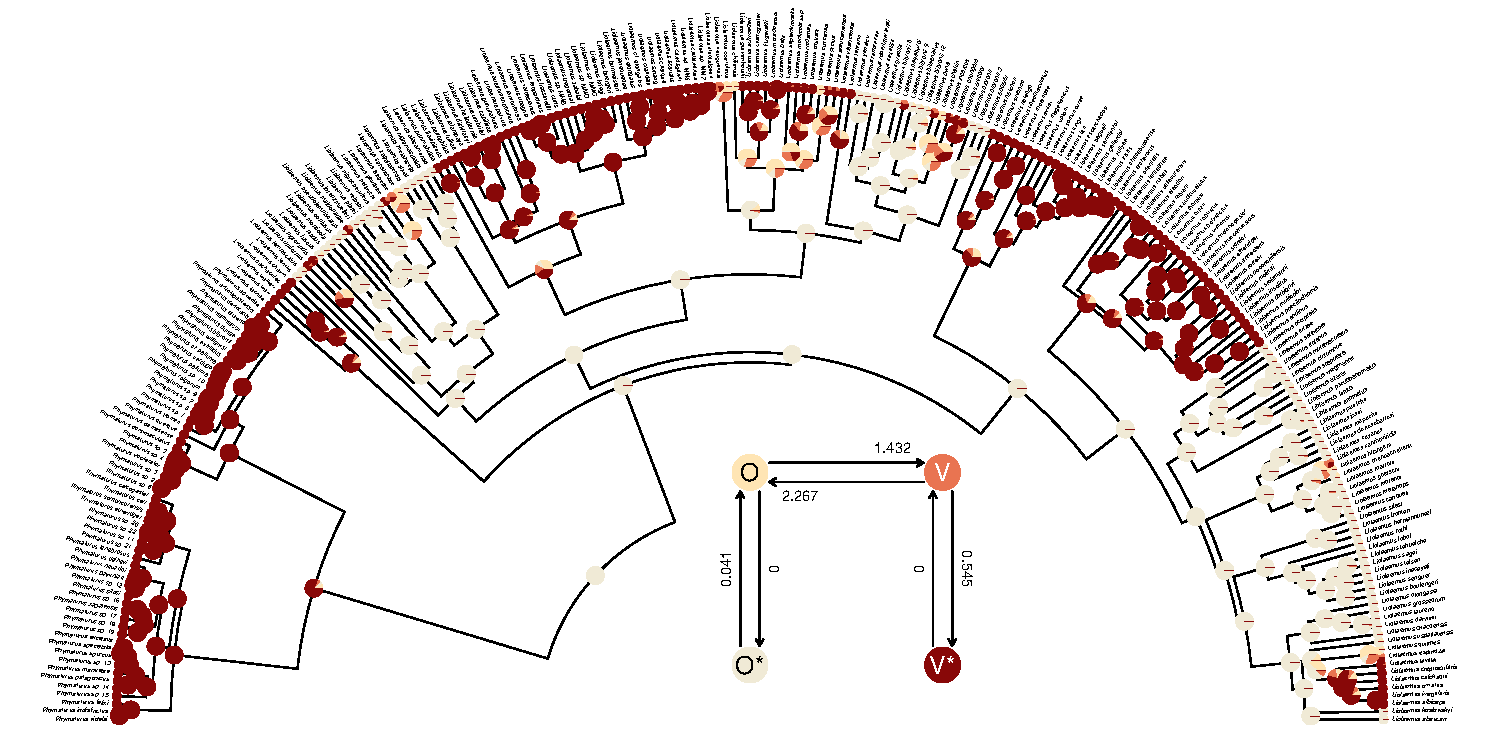
\includegraphics[width=1\linewidth]{Revell.phytools-v2_peerj_files/figure-latex/anc-fitHRM-1} \caption{\DIFaddFL{Marginal ancestral state reconstruction of parity mode (oviparity vs. viviparity) in liolaemid lizards under the hidden-rates model. Phylogeny and data based on Esquerr\'e et al. (2019). Inset panel shows best-supported hidden-rates model. See main text for additional details.}}\label{fig:anc-fitHRM}
\end{figure}

\DIFaddend \hypertarget{continuous-characters}{%
\section{Continuous characters}\label{continuous-characters}}

Numerous continuous trait methods exist in the \emph{phytools} package.
For example, \emph{phytools} can be used to measure phylogenetic signal
(\texttt{phylosig}, Pagel 1999; Blomberg et al. 2003; Revell et al.
2008), it can fit multi-rate Brownian evolution models
(\texttt{brownie.lite}, \texttt{brownieREML}, \texttt{evol.rate.mcmc},
\texttt{multirateBM}, \texttt{ratebytree}, and \texttt{rateshift},
O'Meara et al. 2006; Revell et al. 2012, 2018; Revell 2021; Revell and
Harmon 2022), it can perform phylogenetic canonical correlation and
principal components analysis (\texttt{phyl.cca} and \texttt{phyl.pca},
Revell and Harrison 2008; Revell 2009), it can reconstruct ancestral
states under multiple evolutionary models (\texttt{anc.Bayes},
\texttt{anc.ML}, \texttt{anc.trend}, and \texttt{fastAnc}, Schluter et
al. 1997; Revell and Harmon 2022), it can use continuous trait data to
place a fossil or missing lineage into a reconstructed tree
(\texttt{locate.fossil} and \texttt{locate.yeti}, Felsenstein 2002;
Revell et al. 2015), it can fit a multivariate Brownian model with
multiple evolutionary correlations on the tree (\texttt{evol.vcv} and
\texttt{evolvcv.lite}, Revell and Collar 2009; Revell et al. 2022), and
it can perform various types of continuous character numerical
simulation on phylogenies (e.g., \texttt{branching.diffusion},
\texttt{fastBM}, \texttt{sim.corrs}, \texttt{sim.rates}).

Here I'll start by illustrating the measurement of phylogenetic signal
(\texttt{phylosig}), then I'll demonstrate Bayesian ancestral state
estimation (\texttt{anc.Bayes}). I'll show how to fit a
variable-correlation multivariate Brownian trait evolution model
(\texttt{evolvcv.lite}), and, finally, I'll demonstrate a relatively new
multi-rate trait evolution model that uses the estimation technique of
penalized likelihood (\texttt{multirateBM}).

\hypertarget{phylogenetic-signal}{%
\subsection{Phylogenetic signal}\label{phylogenetic-signal}}

Perhaps the simplest phylogenetic comparative analysis that we could
choose to undertake for a continuous trait data in R is the measurement
of phylogenetic signal (Pagel 1999; Blomberg et al. 2003; Revell et al.
2008). \DIFdelbegin %DIFDELCMD < 

%DIFDELCMD < %%%
\DIFdelend Phylogenetic signal has been defined in a number of different
ways, but could be considered to be the \DIFdelbegin \DIFdel{simple }\DIFdelend \DIFaddbegin \DIFadd{basic }\DIFaddend tendency of more closely
related species to bear more similarity (one to another) than they do to
more distant taxa \DIFdelbegin \DIFdel{. Phylogenetic signal can be quantified }\DIFdelend \DIFaddbegin \DIFadd{(Revell et al. 2008). Apart from its definition,
phylogenetic signal can likewise be }\emph{\DIFadd{quantified}} \DIFaddend in various
manners\DIFdelbegin \DIFdel{,
but }\DIFdelend \DIFaddbegin \DIFadd{; however, }\DIFaddend undoubtedly the two most popular metrics are Blomberg
et al.'s (2003) \emph{K} statistic, and Pagel's (1999) \(\lambda\).
Conveniently, both of these can be calculated using the \emph{phytools}
package.

To get started in this undertaking, let's load some data from
\emph{phytools} consisting of a phylogenetic tree of elopomorph eels and
a data frame of phenotypic traits. Both tree and data were obtained from
an article by Collar et al. (2014) \DIFaddbegin \DIFadd{and are now packaged with
}\emph{\DIFadd{phytools}}\DIFaddend .

\begin{Shaded}
\begin{Highlighting}[]
\FunctionTok{data}\NormalTok{(eel.tree)}
\FunctionTok{data}\NormalTok{(eel.data)}
\FunctionTok{head}\NormalTok{(eel.data)}
\end{Highlighting}
\end{Shaded}

\begin{verbatim}
##                   feed_mode Max_TL_cm
## Albula_vulpes       suction       104
## Anguilla_anguilla   suction        50
## Anguilla_bicolor    suction       120
## Anguilla_japonica   suction       150
## Anguilla_rostrata   suction       152
## Ariosoma_anago      suction        60
\end{verbatim}

Having loaded these data, we\DIFdelbegin \DIFdel{can }\DIFdelend \DIFaddbegin \DIFadd{'ll }\DIFaddend next extract one variable from our data
array. Phylogenetic signal can be measured for any continuous trait, so
we'll use maximum total length: here represented by the column of our
data frame called \texttt{"Max\_TL\_cm"}. As is often the case, we'll
transform our data to a log scale. (There are multiple reasons log
transformations are favored by comparative biologists working on
interspecies data. One is that it makes a, say, 10\% change equal,
regardless of whether it occurs in an elephant or a mouse! See Revell
and Harmon 2022 for more details.)

\begin{Shaded}
\begin{Highlighting}[]
\NormalTok{eel.lnTL}\OtherTok{\textless{}{-}}\FunctionTok{setNames}\NormalTok{(}\FunctionTok{log}\NormalTok{(eel.data}\SpecialCharTok{$}\NormalTok{Max\_TL\_cm),}
  \FunctionTok{rownames}\NormalTok{(eel.data))}
\end{Highlighting}
\end{Shaded}

Next, we'll compute a value of the \emph{K} statistic of Blomberg et al.
(2003) using the \emph{phytools} function \texttt{phylosig}.
\texttt{phylosig} calculates \emph{K} by default (that is, without
specifying an argument for \texttt{method}), but if I add the argument
value \texttt{test=TRUE}, \texttt{phylosig} will also conduct a
statistical test of the measured value of \emph{K} by comparing it to a
null distribution of \emph{K} obtained by permuting our observed trait
values randomly across the tips of the phylogeny.

\begin{Shaded}
\begin{Highlighting}[]
\NormalTok{eel.Blomberg\_K}\OtherTok{\textless{}{-}}\FunctionTok{phylosig}\NormalTok{(eel.tree,eel.lnTL,}\AttributeTok{test=}\ConstantTok{TRUE}\NormalTok{)}
\NormalTok{eel.Blomberg\_K}
\end{Highlighting}
\end{Shaded}

\DIFmodbegin
\begin{DIFverbatim}[alsolanguage=DIFcode]
## 
## Phylogenetic signal K : 0.362879 
%DIF < ## P-value (based on 1000 randomizations) : 0.033
%DIF > ## P-value (based on 1000 randomizations) : 0.036
\end{DIFverbatim}
\DIFmodend

\emph{K} has an expected value of 1.0 under Brownian motion (Blomberg et
al. 2003). The lower value that we observe here thus indicates less
phylogenetic signal than expected under Brownian evolution; whereas a
value higher than 1.0 would've indicated more. Our significance test
shows us that this value of \emph{K}, though \DIFaddbegin \DIFadd{numerically }\DIFaddend modest, is
nonetheless significantly greater than we'd expect to find in data that
were entirely random with respect to the tree!

In addition to Blomberg et al.'s \emph{K}, \emph{phytools} also can be
used to estimate Pagel's (1999) \(\lambda\) statistic. \(\lambda\)
measures phylogenetic signal as a scalar multiplier of the correlations
of related taxa in our tree (Revell and Harmon 2022). That is to say, if
\(\lambda\) has a value less than 1.0, this would indicate that related
species in our phylogeny have a lower degree of ``autocorrelation'' than
expected under Brownian evolution. In fact, a value of \(\lambda\) close
to zero could be taken to indicate that related species are not
phenotypically correlated at all!

We use Maximum Likelihood to find the value of \(\lambda\) that makes
our observed data most probable. Since it's \DIFdelbegin \DIFdel{possible }\DIFdelend \DIFaddbegin \DIFadd{straightforward }\DIFaddend to compute a
likelihood for any allowable value of \(\lambda\), including \(\lambda\)
= 0, we can very easily proceed to test a null hypothesis of no
phylogenetic signal in our data by simply calculating a likelihood ratio
in which we compare \(\lambda\) = 0 to our Maximum Likelihood estimate.
Indeed, this is the test performed by \emph{phytools} if
\texttt{method="lambda"} and \texttt{test=TRUE}!

\begin{Shaded}
\begin{Highlighting}[]
\NormalTok{eel.Pagel\_lambda}\OtherTok{\textless{}{-}}\FunctionTok{phylosig}\NormalTok{(eel.tree,eel.lnTL,}
  \AttributeTok{method=}\StringTok{"lambda"}\NormalTok{,}\AttributeTok{test=}\ConstantTok{TRUE}\NormalTok{)}
\NormalTok{eel.Pagel\_lambda}
\end{Highlighting}
\end{Shaded}

\begin{verbatim}
## 
## Phylogenetic signal lambda : 0.673729 
## logL(lambda) : -54.3016 
## LR(lambda=0) : 5.18173 
## P-value (based on LR test) : 0.0228256
\end{verbatim}

This result tells us that we've found significant phylogenetic signal in
our trait by both measures. Although \emph{K} and \(\lambda\) tend to be
correlated, it's entirely possible that we could've found significant
\emph{K} and non-significant \(\lambda\), or vice versa. This is not a
contradiction. The concept of phylogenetic signal is one of phenotypic
similarity among related species -- but \emph{K} and \(\lambda\) measure
this concept via two entirely different procedures!

Along with the simple calculation of phylogenetic signal,
\emph{phytools} also contains several methods to visualize our results.
In particular, for Blomberg et al.'s \emph{K} we can plot the
permutation distribution of \emph{K} alongside our observed measure. For
Pagel's \(\lambda\), we can plot the likelihood surface, our Maximum
Likelihood solution, and the likelihood of \(\lambda\) = 0: the null
hypothesis of our statistical tests. Both of these plots are illustrated
in Figure @ref(fig:phylosig) for our eel body length data.

\begin{Shaded}
\begin{Highlighting}[]
\FunctionTok{par}\NormalTok{(}\AttributeTok{mfrow=}\FunctionTok{c}\NormalTok{(}\DecValTok{1}\NormalTok{,}\DecValTok{2}\NormalTok{),}\AttributeTok{cex=}\FloatTok{0.9}\NormalTok{)}
\FunctionTok{plot}\NormalTok{(eel.Blomberg\_K,}\AttributeTok{las=}\DecValTok{1}\NormalTok{,}\AttributeTok{cex.axis=}\FloatTok{0.9}\NormalTok{)}
\FunctionTok{mtext}\NormalTok{(}\StringTok{"a)"}\NormalTok{,}\AttributeTok{adj=}\DecValTok{0}\NormalTok{,}\AttributeTok{line=}\DecValTok{1}\NormalTok{)}
\FunctionTok{plot}\NormalTok{(eel.Pagel\_lambda,}\AttributeTok{bty=}\StringTok{"n"}\NormalTok{,}\AttributeTok{las=}\DecValTok{1}\NormalTok{,}\AttributeTok{cex.axis=}\FloatTok{0.9}\NormalTok{,}
  \AttributeTok{xlim=}\FunctionTok{c}\NormalTok{(}\DecValTok{0}\NormalTok{,}\FloatTok{1.1}\NormalTok{))}
\FunctionTok{mtext}\NormalTok{(}\StringTok{"b)"}\NormalTok{,}\AttributeTok{adj=}\DecValTok{0}\NormalTok{,}\AttributeTok{line=}\DecValTok{1}\NormalTok{)}
\end{Highlighting}
\end{Shaded}

\begin{figure}
\DIFdelbeginFL %DIFDELCMD < 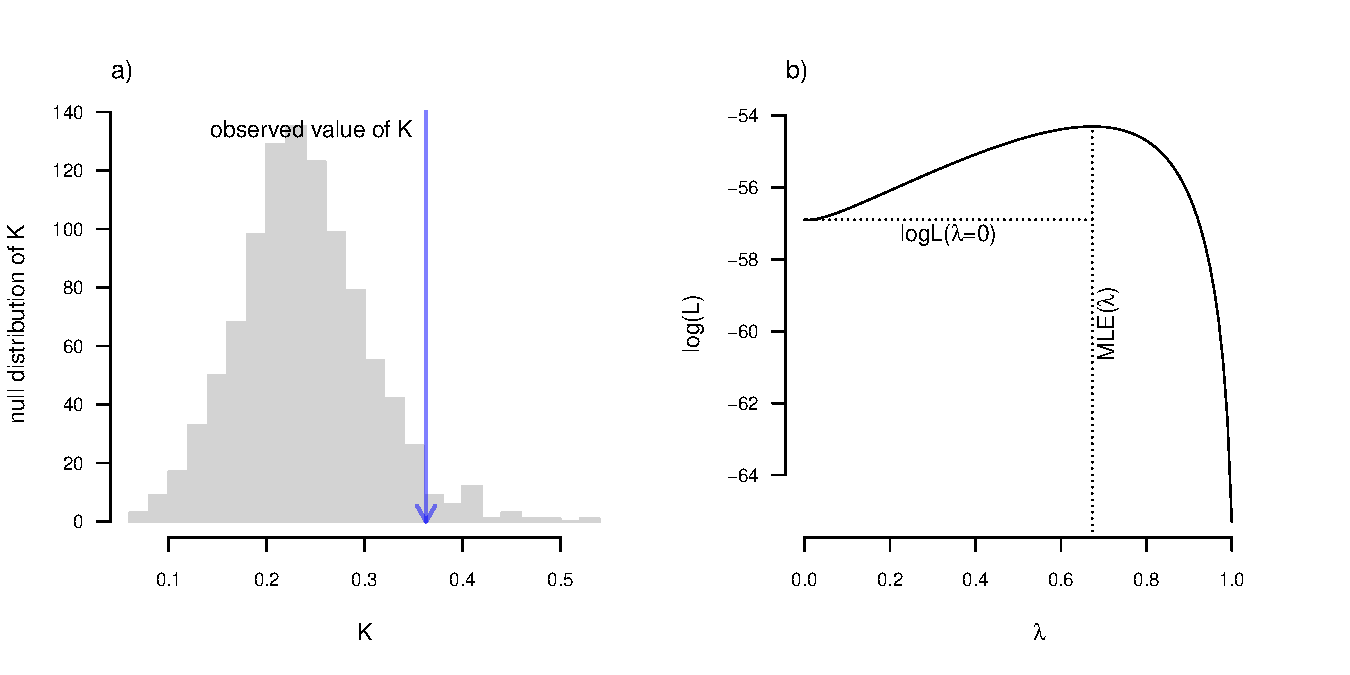
\includegraphics[width=1\linewidth]{old.Revell.phytools-v2_peerj_files/figure-latex/phylosig-1} %%%
\DIFdelendFL \DIFaddbeginFL 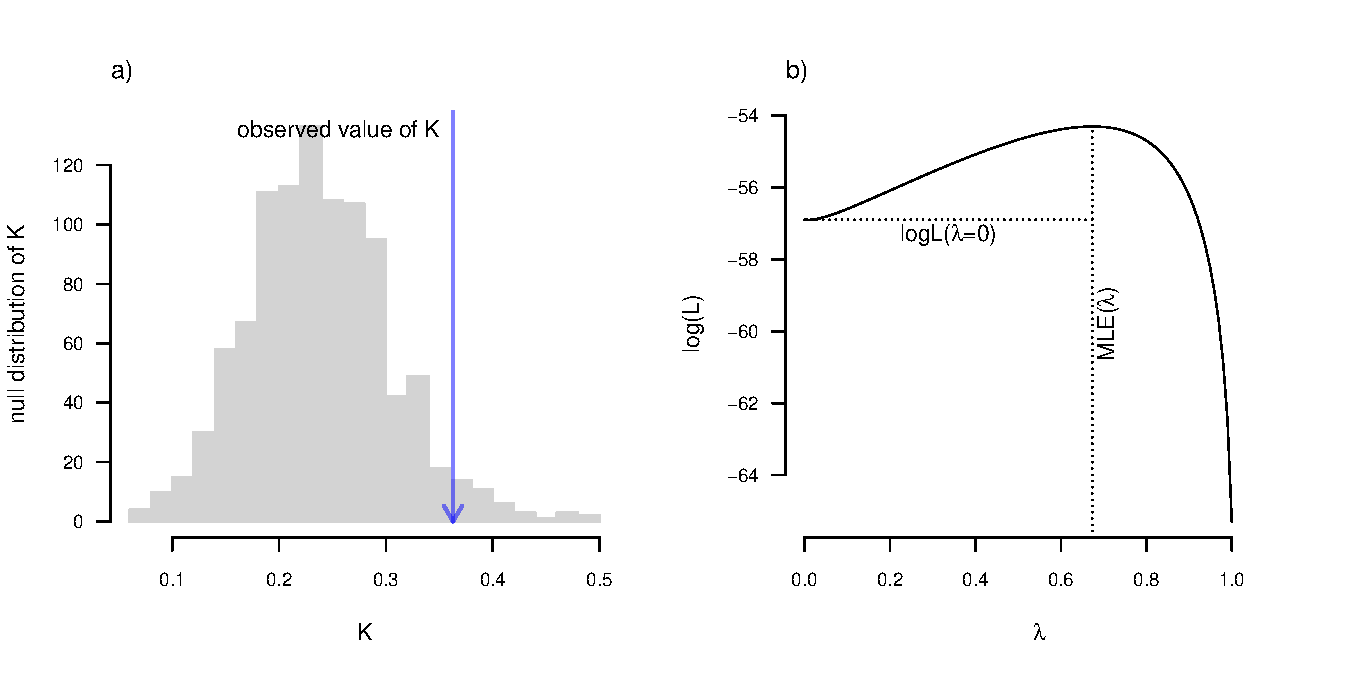
\includegraphics[width=1\linewidth]{Revell.phytools-v2_peerj_files/figure-latex/phylosig-1} \DIFaddendFL \caption{a) Blomberg et al. (2003) measured value of the \textit{K} statistic for phylogenetic signal, compared to a null distribution of \textit{K} obtained via randomization. b) Pagel's (1999) $\lambda$ statistic for phylogenetic signal, also showing the likelihood surface. Data consist of maximum body length (on a log scale) from 61 species of elopomorph eels \DIFaddbeginFL \DIFaddFL{(Collar et al}\DIFaddendFL . \DIFaddbeginFL \DIFaddFL{2014). }\DIFaddendFL See main text for additional details.}\label{fig:phylosig}
\end{figure}

\hypertarget{bayesian-ancestral-state-estimation}{%
\subsection{Bayesian ancestral state
estimation}\label{bayesian-ancestral-state-estimation}}

The \emph{phytools} package contains several different functions for
discrete and continuous character ancestral state estimation under
multiple models. Earlier, we reviewed the method of stochastic character
mapping (Huelsenbeck et al. 2003) \DIFdelbegin \DIFdel{which can be an important tool }\DIFdelend \DIFaddbegin \DIFadd{and marginal ancestral character
estimation, both of which are important tools }\DIFaddend for ancestral state
reconstruction of \DIFdelbegin \DIFdel{discrete characters}\DIFdelend \DIFaddbegin \DIFadd{discretely-valued traits}\DIFaddend .

Among the variety of approaches for ancestral character estimation of
continuous characters that are implemented in the \emph{phytools}
package is the function \texttt{anc.Bayes}. As its name suggests,
\texttt{anc.Bayes} performs ancestral state estimation using Bayesian
MCMC. Just as any proper Bayesian approach should, the implementation of
this method allows us to include prior information about the states at
internal nodes. Here, I'll illustrate the simplest type of analysis that
we can undertake with the function in which I'll simply accept the
default node priors and MCMC conditions. \texttt{anc.Bayes}, however,
will be most useful when we intend to explicitly incorporate prior
knowledge about internal nodes of the tree -- based on, for instance,
observations from the fossil record.

To demonstrate the method, I'll load a dataset (now packaged with
\emph{phytools}) that consists of a phylogeny and phenotypic trait
information for a set of lizards from the family Cordylidae, originally
published by Broeckhoven et al. (2016).

\begin{Shaded}
\begin{Highlighting}[]
\FunctionTok{data}\NormalTok{(cordylid.tree)}
\FunctionTok{data}\NormalTok{(cordylid.data)}
\FunctionTok{head}\NormalTok{(cordylid.data)}
\end{Highlighting}
\end{Shaded}

\begin{verbatim}
##                    pPC1     pPC2     pPC3
## C._aridus       0.59441 -0.40209  0.57109
## C._minor        0.65171 -0.32732  0.55692
## C._imkeae       0.19958 -0.08978  0.56671
## C._mclachlani   0.62065  0.03746  0.86721
## C._macropholis  0.44875 -0.75942  0.09737
## C._cordylus    -0.07267  0.48294 -0.54394
\end{verbatim}

Our trait data in this case are species scores for three different
principal component (PC) axes from a phylogenetic principal components
analysis undertaken using the \emph{phytools} \texttt{phyl.pca} function
(Revell 2009). Cordylid lizards are known for their body and tail armor,
consisting of large, rectangular scales called osteoderms. Principal
component 1 in Broeckhoven et al. (2016) separated the most lightly
armored cordylids (large negative values), from those cordylids with the
heaviest body armor (large positive values of PC 1). Why don't we
extract this principal component from our data frame and rename it, as
follows?

\begin{Shaded}
\begin{Highlighting}[]
\NormalTok{cordylid.armor\_score}\OtherTok{\textless{}{-}}\FunctionTok{setNames}\DIFdelbegin \DIFdel{\NormalTok{(}
\NormalTok{  cordylid.data}}\DIFdelend \DIFaddbegin \DIFadd{\NormalTok{(cordylid.data}}\DIFaddend \SpecialCharTok{$}\NormalTok{pPC1,}
  \FunctionTok{rownames}\NormalTok{(cordylid.data))}
\end{Highlighting}
\end{Shaded}

With this named trait vector at the ready, we're prepared to undertake
our Bayesian MCMC. As noted above, we'll use the default conditions but
update the number of generations that we want our MCMC to run to
\texttt{ngen=500000}. Depending on the size of our phylogenetic tree, we
may want to run more (or fewer) generations in a genuine empirical
study.

\begin{Shaded}
\begin{Highlighting}[]
\NormalTok{cordylid.mcmc}\OtherTok{\textless{}{-}}\FunctionTok{anc.Bayes}\NormalTok{(cordylid.tree,}
\NormalTok{  cordylid.armor\_score,}\AttributeTok{ngen=}\DecValTok{500000}\NormalTok{)}
\end{Highlighting}
\end{Shaded}

\begin{verbatim}
## List of 7
##  $ sig2   : num 0.713
##  $ a      : num [1, 1] 0.000422
##  $ y      : num [1:26] 0.000422 0.000422 0.000422 0.000422 ...
##  $ pr.mean: num [1:28] 1000 0 0 0 0 0 0 0 0 0 ...
##  $ pr.var : num [1:28] 1e+06 1e+03 1e+03 1e+03 1e+03 ...
##  $ prop   : num [1:28] 0.00713 0.00713 0.00713 0.00713 ...
##  $ sample : num 100

## Starting MCMC...

## Done MCMC.
\end{verbatim}

We can see that the method starts by printing out a summary of the
``control parameters'' of the MCMC. These include\DIFaddbegin \DIFadd{: initial values for
the Brownian rate, \(\sigma^{2}\) (}\texttt{\DIFadd{sig2}}\DIFadd{), the root state
(}\texttt{\DIFadd{a}}\DIFadd{), and the internal node values (}\texttt{\DIFadd{y}}\DIFadd{); }\DIFaddend information
about our prior probability distributions \DIFdelbegin \DIFdel{, }\DIFdelend \DIFaddbegin \DIFadd{(}\texttt{\DIFadd{pr.mean}} \DIFadd{and
}\texttt{\DIFadd{pr.var}}\DIFadd{); }\DIFaddend the variances of the proposal distributions \DIFdelbegin \DIFdel{, }\DIFdelend \DIFaddbegin \DIFadd{on each
variable in the model (}\texttt{\DIFadd{prop}}\DIFadd{); }\DIFaddend and, finally, the interval that
we'll use to sample from our posterior \DIFaddbegin \DIFadd{distribution during the MCMC
(}\texttt{\DIFadd{sample}}\DIFadd{)}\DIFaddend . All of these parameters can be adjusted by the
\emph{phytools} user.

The object class that results from this function call
(\texttt{"anc.Bayes"}) has a \texttt{summary} method in \emph{phytools}
that prints the mean from the posterior distribution, automatically
excluding the first 20\% of our samples as burn-in (though we can adjust
this percentage if we'd like). \DIFdelbegin \DIFdel{It }\DIFdelend \DIFaddbegin \DIFadd{Though a thorough review of Bayesian MCMC
is beyond the scope of this article, burn-in refers to the number of
generations required for our MCMC to convergence on the posterior
probability distribution, and will depend on numerous factors including
(but not limited to) our starting values, the parameter complexity of
our model, and the proposal distribution. (See Roy 2020 for a recent
review of burn-in, convergence diagnostics, and related topics.)
Convergence can be diagnosed quantitatively via multiple methods,
including using the R package }\emph{\DIFadd{coda}} \DIFadd{(Plummer et al. 2006). In
addition to printing our results to screen, }\texttt{\DIFadd{summary}} \DIFaddend also passes
the estimates (normally invisibly, but we can save them to a new
variable in our workspace as we've done here) back to the user.

\begin{Shaded}
\begin{Highlighting}[]
\NormalTok{cordylid.ace}\OtherTok{\textless{}{-}}\FunctionTok{summary}\NormalTok{(cordylid.mcmc)}
\end{Highlighting}
\end{Shaded}

\begin{verbatim}
## 
## Object of class "anc.Bayes" consisting of a posterior
##    sample from a Bayesian ancestral state analysis:
## 
## Mean ancestral states from posterior distribution:
##        29        30        31        32        33        34 
##  0.059277 -0.099027 -0.106452  0.057220  0.153671  0.201722 
##        35        36        37        38        39        40 
##  0.225081  0.297659  0.392992  0.493316  0.015503 -0.006053 
##        41        42        43        44        45        46 
##  0.435309  0.392526  0.300532  0.210391 -1.505181 -1.857682
##        47        48        49        50        51        52
## -0.136014 -0.520322 -0.829181 -0.985510 -1.040208  0.385293
##        53        54        55 
##  0.511646  0.159943  0.028358 
## 
## Based on a burn-in of 1e+05 generations.
\end{verbatim}

Now that we've obtained our estimated Bayesian ancestral states for
internal nodes, it's a straightforward task to visualize them on the
branches and nodes of the tree. For this undertaking we'll use the
popular \emph{phytools} plotting function \texttt{contMap} (Revell
2013). By default, \texttt{contMap} uses Maximum Likelihood to compute
ancestral states at all of the internal nodes of the tree -- but it can
also be supplied with user-specified values. Since we want to use our
Bayesian estimates from \texttt{anc.Bayes}, that's what we'll do here.

\begin{Shaded}
\begin{Highlighting}[]
\NormalTok{cordylid.contMap}\OtherTok{\textless{}{-}}\FunctionTok{contMap}\NormalTok{(cordylid.tree,}
\NormalTok{  cordylid.armor\_score,}\AttributeTok{anc.states=}\NormalTok{cordylid.ace,}
  \AttributeTok{plot=}\ConstantTok{FALSE}\NormalTok{)}
\NormalTok{cordylid.contMap}\OtherTok{\textless{}{-}}\FunctionTok{setMap}\NormalTok{(cordylid.contMap,}
\NormalTok{  viridisLite}\SpecialCharTok{::}\FunctionTok{viridis}\NormalTok{(}\AttributeTok{n=}\DecValTok{10}\NormalTok{,}\AttributeTok{direction=}\SpecialCharTok{{-}}\DecValTok{1}\NormalTok{))}
\FunctionTok{plot}\NormalTok{(cordylid.contMap,}\AttributeTok{ftype=}\StringTok{"i"}\NormalTok{,}\AttributeTok{fsize=}\FunctionTok{c}\NormalTok{(}\FloatTok{0.6}\NormalTok{,}\DIFdelbegin \DIFdel{\FloatTok{0.8}}\DIFdelend \DIFaddbegin \DIFadd{\FloatTok{0.7}}\DIFaddend \NormalTok{),}
  \AttributeTok{leg.txt=}\StringTok{"PC 1 (increasing armor)"}\NormalTok{,}\AttributeTok{lwd=}\DecValTok{3}\NormalTok{)}
\FunctionTok{nodelabels}\NormalTok{(}\AttributeTok{frame=}\StringTok{"circle"}\NormalTok{,}\AttributeTok{bg=}\StringTok{"white"}\NormalTok{,}\AttributeTok{cex=}\FloatTok{0.6}\NormalTok{)}
\end{Highlighting}
\end{Shaded}

\begin{figure}
\DIFdelbeginFL %DIFDELCMD < 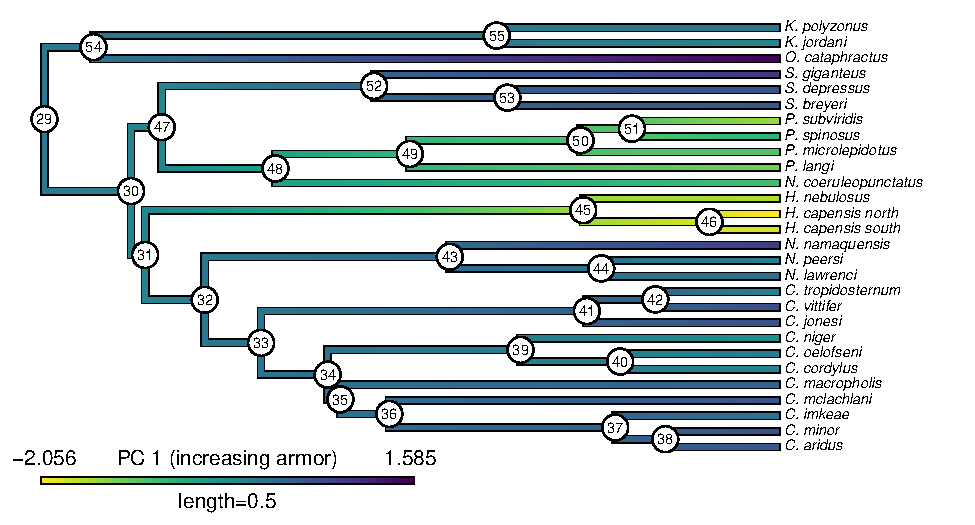
\includegraphics[width=1\linewidth]{old.Revell.phytools-v2_peerj_files/figure-latex/cordylid-ace-1} %%%
\DIFdelendFL \DIFaddbeginFL 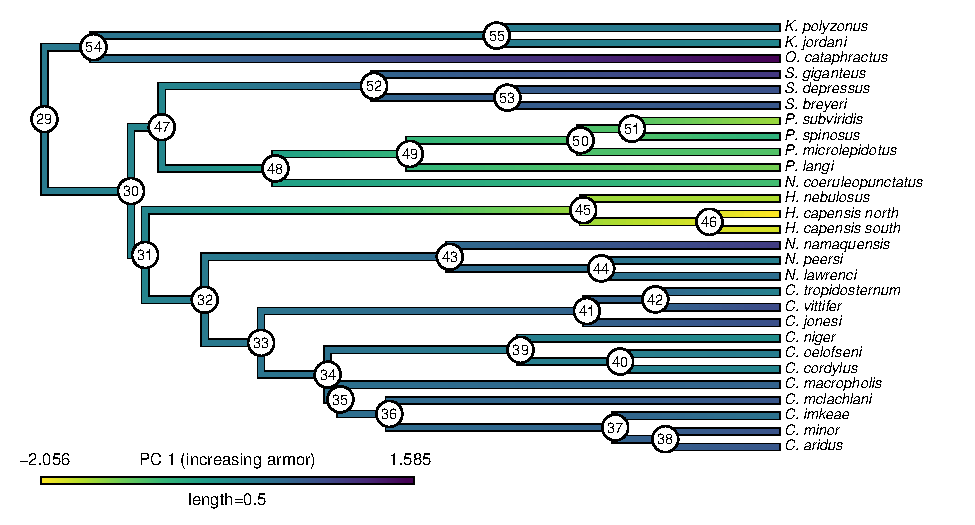
\includegraphics[width=1\linewidth]{Revell.phytools-v2_peerj_files/figure-latex/cordylid-ace-1} \DIFaddendFL \caption{Reconstructed ancestral values from Bayesian MCMC projected onto the nodes and edges of the tree. Numerical values at internal nodes are node indices from our input phylogeny. Data consist of PC 1 from a phylogenetic principal components analysis of cordylid morphological \DIFdelbeginFL \DIFdelFL{trait}\DIFdelendFL \DIFaddbeginFL \DIFaddFL{traits}\DIFaddendFL , and separate highly armored (high values) from lightly armored (low values) lizards \DIFaddbeginFL \DIFaddFL{(Broeckhoven et al}\DIFaddendFL . \DIFaddbeginFL \DIFaddFL{2016). }\DIFaddendFL See main text for more details.}\label{fig:cordylid-ace}
\end{figure}

\DIFdelbegin \DIFdel{(}\DIFdelend For fun, compare Figure @ref(fig:cordylid-ace) to Figure 2 of
Broeckhoven et al.~in which estimated ancestral state values were
assigned to each branch using a similar color gradient!
\DIFdelbegin \DIFdel{)
}\DIFdelend 

In addition to this simple analysis, we can (naturally) extract and plot
posterior probability densities from any of our internal nodes of the
tree. To see this, let's focus on the node labeled ``49'' in Figure
@ref(fig:cordylid-ace) and do exactly that. Node 49 corresponds to the
common ancestor of the \emph{Pseudocordylus} clade\DIFdelbegin \DIFdel{, which is among the least heavily armored of all cordylids in
our tree}\DIFdelend \DIFaddbegin \DIFadd{. The
}\emph{\DIFadd{Pseudocordylus}} \DIFadd{are among the most lightly all cordylid lizards in
this analysis}\DIFaddend , so we'd expect our posterior distribution for this node
to be centered on a relatively low value \DIFdelbegin \DIFdel{for }\DIFdelend \DIFaddbegin \DIFadd{of }\DIFaddend our armor score.

\begin{Shaded}
\begin{Highlighting}[]
\NormalTok{cordylid.node49}\OtherTok{\textless{}{-}}\FunctionTok{density}\NormalTok{(cordylid.mcmc,}\AttributeTok{what=}\DecValTok{49}\NormalTok{)}
\NormalTok{cordylid.node49}
\end{Highlighting}
\end{Shaded}

\begin{verbatim}
## 
## Call:
##  density.anc.Bayes(x = cordylid.mcmc, what = 49)
## 
## Data: node 49 (4001 obs.);   Bandwidth 'bw' = 0.05679
## 
##        x                 y           
##  Min.   :-2.1658   Min.   :0.000023  
##  1st Qu.:-1.5270   1st Qu.:0.022415  
##  Median :-0.8883   Median :0.187932  
##  Mean   :-0.8883   Mean   :0.391002  
##  3rd Qu.:-0.2495   3rd Qu.:0.784591  
##  Max.   : 0.3893   Max.   :1.187968
\end{verbatim}

\begin{Shaded}
\begin{Highlighting}[]
\FunctionTok{par}\NormalTok{(}\AttributeTok{mar=}\FunctionTok{c}\NormalTok{(}\FloatTok{5.1}\NormalTok{,}\FloatTok{4.1}\NormalTok{,}\FloatTok{1.1}\NormalTok{,}\FloatTok{2.1}\NormalTok{))}
\FunctionTok{plot}\NormalTok{(cordylid.node49,}\AttributeTok{las=}\DecValTok{1}\NormalTok{,}\AttributeTok{bty=}\StringTok{"n"}\NormalTok{,}\AttributeTok{main=}\StringTok{""}\NormalTok{,}\AttributeTok{cex.lab=}\DIFdelbegin \DIFdel{\FloatTok{0.9}\NormalTok{,}
  \AttributeTok{cex.axis=}\FloatTok{0.8}}\DIFdelend \DIFaddbegin \DIFadd{\FloatTok{0.8}\NormalTok{,}
  \AttributeTok{cex.axis=}\FloatTok{0.7}}\DIFaddend \NormalTok{,}\AttributeTok{xlab=}\StringTok{"PC 1 (increasing armor)"}\NormalTok{,}
  \AttributeTok{ylab=}\StringTok{"Posterior density"}\NormalTok{,}
  \AttributeTok{xlim=}\FunctionTok{range}\NormalTok{(cordylid.armor\_score))}
\end{Highlighting}
\end{Shaded}

\begin{figure}
\DIFdelbeginFL %DIFDELCMD < \includegraphics[width=1\linewidth]{old.Revell.phytools-v2_peerj_files/figure-latex/cordylid-pd-1} %%%
\DIFdelendFL \DIFaddbeginFL \includegraphics[width=1\linewidth]{Revell.phytools-v2_peerj_files/figure-latex/cordylid-pd-1} \DIFaddendFL \caption{Posterior probability density at node 49 of Figure 10 from Bayesian MCMC ancestral state reconstruction of PC 1 from a morphological analysis on a phylogenetic tree of cordylid lizards. Node 49 corresponds to the common ancestor of the \textit{Pseudocordylus}: a relatively lightly armored cordylid clade. See main text for more details.}\label{fig:cordylid-pd}
\end{figure}

Figure @ref(fig:cordylid-pd) shows our estimate of the posterior
probability distribution of the ancestral node 49 state, and should be
centered precisely on the value we projected onto the tree of Figure
@ref(fig:cordylid-ace)!

\DIFaddbegin \DIFadd{As given here, Bayesian MCMC ancestral state reconstruction will yield
(in nearly all circumstances) point estimates that are highly similar to
the values that we might have obtained using Maximum Likelihood.
Nonetheless, Bayesian inference provides the additional benefit of
supplying a natural framework for incorporating prior information about
the states at one or various internal nodes in the tree (by adjusting
}\texttt{\DIFadd{pr.mean}}\DIFadd{, }\texttt{\DIFadd{pr.var}}\DIFadd{, or both: see above), as well as for
measuring the substantial uncertainty that can be associated with
ancestral trait estimates (in particular, by providing not just
confidence intervals around each node, but sets of ancestral values
across }\emph{\DIFadd{all}} \DIFadd{nodes of the tree that have been sampled in proportion
to their posterior probability under the model).
}

\DIFaddend \hypertarget{multivariate-trait-evolution}{%
\subsection{Multivariate trait
evolution}\label{multivariate-trait-evolution}}

Along with the various univariate methods we've seen so far,
\emph{phytools} also contains a handful of different multivariate trait
evolution models, designed for both continuous and discrete characters.

One of these is an interesting model (described in Revell and Collar
2009; Revell et al. 2022) in which the rates and evolutionary
correlations between traits are allowed to vary as a function of a set
of mapped regimes on the tree. (Similar to O'Meara et al. 2006, but for
more than one trait at a time.) The underlying motivation of this method
is to test hypotheses about phylogenetic heterogeneity in the
evolutionary relationship (i.e., correlation) between different traits
on our phylogeny. \DIFaddbegin \DIFadd{This approach is also used to study quantitative trait
modularity and integration during macroevolution (e.g., Damian-Serrano
et al. 2021).
}\DIFaddend 

\DIFdelbegin \DIFdel{To illustrate the method, }\DIFdelend \DIFaddbegin \DIFadd{Note that closely related analyses have been implemented in the R
packages }\emph{\DIFadd{mvMORPH}} \DIFadd{by Clavel et al. (2015), and }\emph{\DIFadd{ratematrix}}
\DIFadd{by Caetano and Harmon (2017). The packages }\emph{\DIFadd{mvSLOUCH}} \DIFadd{(Bartoszek et
al. 2012), }\emph{\DIFadd{PhylogeneticEM}} \DIFadd{(Bastide et al. 2018), and
}\emph{\DIFadd{PCMFit}} \DIFadd{(Mitov et al. 2019) also feature phylogenetic multivariate
quantitative trait analysis methods.
}

\DIFadd{To illustrate our approach, however, }\DIFaddend I'll use a phylogenetic tree and
dataset of tropidurid lizard species from Revell et al. (2022).

\begin{Shaded}
\begin{Highlighting}[]
\FunctionTok{data}\NormalTok{(tropidurid.tree)}
\FunctionTok{data}\NormalTok{(tropidurid.data)}
\end{Highlighting}
\end{Shaded}

In this case, our phylogeny is already a tree with mapped regimes. We
can see this by merely printing the model object that we loaded. (In an
empirical study we might imagine using a set of such trees sampled in
proportion to their probabilities using stochastic mapping -- and then
averaging the result. E.g., see Revell et al. 2022.)

\begin{Shaded}
\begin{Highlighting}[]
\FunctionTok{print}\NormalTok{(tropidurid.tree,}\AttributeTok{printlen=}\DecValTok{2}\NormalTok{)}
\end{Highlighting}
\end{Shaded}

\DIFmodbegin
\begin{DIFverbatim}[alsolanguage=DIFcode]
## 
## Phylogenetic tree with 76 tips and 75 internal nodes.
## 
## Tip labels:
##  Leiocephalus_raviceps, Leiocephalus_carinatus, ...
## 
## The tree includes a mapped, 2-state discrete character
## with states:
%DIF < ##  n_rock, rock
%DIF > ##  non-rock dwelling, rock-dwelling
## 
## Rooted; includes branch lengths.
\end{DIFverbatim}
\DIFmodend

This tells us that our phylogenetic tree contains 76 taxa and a mapped
regime with two states: \texttt{"n\_rock"} (non-rock dwelling) and
\texttt{"rock"} (rock-dwelling). Since \emph{phytools} permits mapped
regimes to have \DIFdelbegin \DIFdel{arbitrary }\DIFdelend \DIFaddbegin \DIFadd{arbitrarily lengthy }\DIFaddend names, let's rename these \DIFaddbegin \DIFadd{two regime
}\DIFaddend levels in a more informative way. To do so, I'll use the \emph{phytools}
function \texttt{\DIFdelbegin \DIFdel{mergeMappedTraits}\DIFdelend \DIFaddbegin \DIFadd{mergeMappedStates}\DIFaddend }. \texttt{\DIFdelbegin \DIFdel{mergeMappedTraits}\DIFdelend \DIFaddbegin \DIFadd{mergeMappedStates}\DIFaddend }, as
readers can probably guess, is designed to merge the mappings of two or
more traits into one -- but can also be employed to simply substitute
one mapping name for another\DIFdelbegin \DIFdel{.
}\DIFdelend \DIFaddbegin \DIFadd{!
}\DIFaddend 

\begin{Shaded}
\begin{Highlighting}[]
\NormalTok{tropidurid.tree}\OtherTok{\textless{}{-}}\FunctionTok{mergeMappedStates}\DIFdelbegin \DIFdel{\NormalTok{(}
\NormalTok{  tropidurid.tree,}}\DIFdelend \DIFaddbegin \DIFadd{\NormalTok{(tropidurid.tree,}
  }\DIFaddend \StringTok{"n\_rock"}\NormalTok{,}\StringTok{"non{-}rock dwelling"}\NormalTok{)}
\NormalTok{tropidurid.tree}\OtherTok{\textless{}{-}}\FunctionTok{mergeMappedStates}\DIFdelbegin \DIFdel{\NormalTok{(}
\NormalTok{  tropidurid.tree,}}\DIFdelend \DIFaddbegin \DIFadd{\NormalTok{(tropidurid.tree,}
  }\DIFaddend \StringTok{"rock"}\NormalTok{,}\StringTok{"rock{-}dwelling"}\NormalTok{)}
\end{Highlighting}
\end{Shaded}

Let's plot this updated tree. To do so, I'm going to use the recent
\emph{phytools} function \texttt{sigmoidPhylogram} that will plot our
tree using curved (``sigmoidal'') linking lines. (\emph{phytools}
contains lots of cool \DIFaddbegin \DIFadd{tree plotting }\DIFaddend functions like this one!)

\begin{Shaded}
\begin{Highlighting}[]
\NormalTok{cols}\OtherTok{\textless{}{-}}\FunctionTok{setNames}\NormalTok{(}\FunctionTok{c}\NormalTok{(}\StringTok{"white"}\NormalTok{,}\StringTok{"black"}\NormalTok{),}\FunctionTok{c}\NormalTok{(}\StringTok{"non{-}rock dwelling"}\NormalTok{,}
  \StringTok{"rock{-}dwelling"}\NormalTok{))}
\FunctionTok{sigmoidPhylogram}\NormalTok{(tropidurid.tree,}\AttributeTok{direction=}\StringTok{"upwards"}\NormalTok{,}
  \AttributeTok{outline=}\ConstantTok{TRUE}\NormalTok{,}\AttributeTok{colors=}\NormalTok{cols,}\AttributeTok{direction=}\StringTok{"upwards"}\NormalTok{,}
  \AttributeTok{outline=}\ConstantTok{TRUE}\NormalTok{,}\AttributeTok{lwd=}\DecValTok{2}\NormalTok{,}\AttributeTok{fsize=}\FloatTok{0.4}\NormalTok{,}\AttributeTok{ftype=}\StringTok{"i"}\NormalTok{,}\AttributeTok{offset=}\DecValTok{1}\NormalTok{)}
\FunctionTok{legend}\NormalTok{(}\StringTok{"bottomright"}\NormalTok{,}\FunctionTok{c}\NormalTok{(}\StringTok{"non{-}rock dwelling"}\NormalTok{,}
  \StringTok{"rock{-}dwelling"}\NormalTok{),}\AttributeTok{pch=}\DecValTok{22}\NormalTok{,}\AttributeTok{pt.bg=}\NormalTok{cols,}\AttributeTok{cex=}\FloatTok{0.8}\NormalTok{,}
  \AttributeTok{pt.cex=}\FloatTok{1.2}\NormalTok{)}
\end{Highlighting}
\end{Shaded}

\begin{figure}
\DIFdelbeginFL %DIFDELCMD < \includegraphics[width=1\linewidth]{old.Revell.phytools-v2_peerj_files/figure-latex/trop-tree-1} %%%
\DIFdelendFL \DIFaddbeginFL \includegraphics[width=1\linewidth]{Revell.phytools-v2_peerj_files/figure-latex/trop-tree-1} \DIFaddendFL \caption{Phylogenetic tree of rock- and non-rock dwelling tropidurid lizard species from Revell et al. (2022). \DIFaddbeginFL \DIFaddFL{Mapped colors correspond to a hypothesis of the history of habitat use across the clade. }\DIFaddendFL See main text for more details.}\label{fig:trop-tree}
\end{figure}

\DIFdelbegin \DIFdel{The }\DIFdelend \DIFaddbegin \DIFadd{Our quantitative }\DIFaddend phenotypic trait data in \texttt{tropidurid.data}
consist of a single measure of overall body size (as trait 1,
\texttt{"\DIFdelbegin \DIFdel{new\_size}\DIFdelend \DIFaddbegin \DIFadd{newsize}\DIFaddend "}), and a second metric trait measuring dorsoventral
depth (vs.~flattening, \texttt{"body\_height"}).

\begin{Shaded}
\begin{Highlighting}[]
\FunctionTok{head}\NormalTok{(tropidurid.data)}
\end{Highlighting}
\end{Shaded}

\begin{verbatim}
##                            newsize body_height
## Leiocephalus_raviceps     2.358317  0.05768818
## Leiocephalus_carinatus    2.931721  0.30216220
## Leiocephalus_psammodromus 2.700397  0.19667083
## Leiocephalus_personatus   2.535315  0.32216983
## Leiocephalus_barahonensis 2.473666  0.30266917
## Stenocercus_ochoai        2.549010  0.29067644
\end{verbatim}

Our hypothesis of multivariate trait evolution in this clade is that
these two traits (size and body depth) should generally scale together
in non-rock dwelling lizard species: bigger lizards also tend to have
larger body depths. We hypothesize, however, that this general
relationship may become decoupled in rock-dwelling lineages where the
force of selection is predicted to favor increased flattening, relative
to their non-rock dwelling kin. (There are biomechanical and behavioral
reasons to suspect this could be so. For more information, see Revell et
al. 2007; Revell et al. 2022.)

To test this hypothesis, we'll use the \emph{phytools} function
\texttt{evolvcv.lite} which fits a heirarchical set of models for the
evolutionary rates (of each character) and evolutionary correlations
(between them, Revell \DIFaddbegin \DIFadd{and Collar 2009; Revell }\DIFaddend et al. 2022). \DIFaddbegin \DIFadd{Following
Revell and Collar (2009), these models are: (1) a model with common
rates and correlations between the two discrete traits; (2) a model with
different rates of evolution depending on our mapped state, but a common
correlation; (3) a model with common rates, but a different evolutionary
correlation, depending on the mapped discrete character; and, finally,
(4) a model of different rates and correlations between the two discrete
mapped character states.
}\DIFaddend 

\begin{Shaded}
\begin{Highlighting}[]
\NormalTok{tropidurid.fits}\OtherTok{\textless{}{-}}\FunctionTok{evolvcv.lite}\NormalTok{(tropidurid.tree,}
\NormalTok{  tropidurid.data)}
\end{Highlighting}
\end{Shaded}

\begin{verbatim}
## Fitting model 1: common rates, common correlation...
## Best log(L) from model 1: 52.3056.
## Fitting model 2: different rates, common correlation...
## Best log(L) from model 2: 54.3968.
## Fitting model 3: common rates, different correlation...
## Best log(L) from model 3: 55.1105.
## Fitting model 4: no common structure...
## Best log(L) from model 4: 56.2877.
\end{verbatim}

Having fit each of four models (in this case: \texttt{evolvcv.lite}
actually includes several additional models that we won't review here,
see Revell et al. 2022 for more details), we can most easily compare all
of the models in our set using a generic \texttt{anova} function call as
follows.

\begin{Shaded}
\begin{Highlighting}[]
\FunctionTok{anova}\NormalTok{(tropidurid.fits)}
\end{Highlighting}
\end{Shaded}

\DIFmodbegin
\begin{DIFverbatim}[alsolanguage=DIFcode]
##           log(L) d.f.       AIC     weight
%DIF < ## model 1 52.30560    5 -94.61119 0.09221086
%DIF < ## model 2 54.39681    7 -94.79362 0.10101736
%DIF > ## model 1 52.30560    5 -94.61119 0.09221085
%DIF > ## model 2 54.39681    7 -94.79362 0.10101737
## model 3 55.11048    6 -98.22096 0.56057434
## model 4 56.28765    8 -96.57530 0.24619744
\end{DIFverbatim}
\DIFmodend

This comparison shows us that \DIFaddbegin \DIFadd{our third model (}\DIFaddend \texttt{"model\ 3"}\DIFaddbegin \DIFadd{:
remember, with common rates but different evolutionary correlation
between rock and non-rock dwelling species) }\DIFaddend is the best-supported
explanation of our data in this set\DIFdelbegin \DIFdel{. Indeed, this model }\DIFdelend \DIFaddbegin \DIFadd{, with the lowest AIC score and
highest model weight. We can print out a summary of our set of four
models to review the estimated parameter values of each.
}

\begin{Shaded}
\begin{Highlighting}[]
\DIFadd{\NormalTok{tropidurid.fits}
}\end{Highlighting}
\end{Shaded}

\DIFmodbegin
\begin{DIFverbatim}[alsolanguage=DIFcode]
%DIF > ## Model 1: common rates, common correlation 
%DIF > ##  R[1,1]  R[1,2]  R[2,2]  k   log(L)  AIC
%DIF > ## fitted   0.2224  0.0154  0.0589  5   52.3056 -94.6112    
%DIF > ## 
%DIF > ## (R thinks it has found the ML solution for model 1.)
%DIF > ## 
%DIF > ## Model 2: different rates, common correlation
%DIF > ##  R[1,1]  R[1,2]  R[2,2]  k   log(L)  AIC
%DIF > ## non-rock dwelling    0.2025  0.0187  0.0456  7   54.3968 -94.7936    
%DIF > ## rock-dwelling    0.3043  0.0382  0.1263  
%DIF > ## 
%DIF > ## (R thinks it has found the ML solution for model 2.)
%DIF > ## 
%DIF > ## Model 3: common rates, different correlation
%DIF > ##  R[1,1]  R[1,2]  R[2,2]  k   log(L)  AIC
%DIF > ## non-rock dwelling    0.2256  0.0394  0.0588  6   55.1105 -98.221 
%DIF > ## rock-dwelling    0.2256  -0.0354 0.0588  
%DIF > ## 
%DIF > ## (R thinks it has found the ML solution for model 3.)
%DIF > ## 
%DIF > ## Model 4: no common structure
%DIF > ##  R[1,1]  R[1,2]  R[2,2]  k   log(L)  AIC
%DIF > ## non-rock dwelling    0.2108  0.0325  0.0485  8   56.2877 -96.5753    
%DIF > ## rock-dwelling    0.2794  -0.0564 0.101   
%DIF > ## 
%DIF > ## (R thinks it has found the ML solution for model 4.)
\end{DIFverbatim}
\DIFmodend

\DIFadd{Here we see that model 3 }\DIFaddend is one in which the evolutionary covariance
between overall body size and dorsoventral flattening is \DIFdelbegin \DIFdel{negative }\DIFdelend \DIFaddbegin \emph{\DIFadd{negative}}
\DIFaddend among rock-dwelling lineages -- compared to the positive evolutionary
covariance in non-rock species and across all other models\DIFdelbegin \DIFdel{, just }\DIFdelend \DIFaddbegin \DIFadd{. Just }\DIFaddend as we'd
predicted\DIFdelbegin \DIFdel{. Size }\DIFdelend \DIFaddbegin \DIFadd{, size }\DIFaddend and body depth are \DIFdelbegin \DIFdel{indeed
}\DIFdelend evolutionarily decoupled in
rock-dwelling \DIFdelbegin \DIFdel{forms}\DIFdelend \DIFaddbegin \DIFadd{specialists}\DIFaddend !

\DIFdelbegin %DIFDELCMD < \begin{Shaded}
%DIFDELCMD < \begin{Highlighting}[]
%DIFDELCMD < %%%
\DIFdel{\NormalTok{tropidurid.fits}
}%DIFDELCMD < \end{Highlighting}
%DIFDELCMD < \end{Shaded}
%DIFDELCMD < 

%DIFDELCMD < \begin{verbatim}
%DIFDELCMD < %%%
%DIFAUXCMD NEXT
\DIFmodbegin
\begin{DIFverbatim}[alsolanguage=DIFcode]
%DIF < ## Model 1: common rates, common correlation 
%DIF < ##  R[1,1]  R[1,2]  R[2,2]  k   log(L)  AIC
%DIF < ## fitted   0.2224  0.0154  0.0589  5   52.3056 -94.6112    
%DIF < ## 
%DIF < ## (R thinks it has found the ML solution for model 1.)
%DIF < ## 
%DIF < ## Model 2: different rates, common correlation
%DIF < ##  R[1,1]  R[1,2]  R[2,2]  k   log(L)  AIC
%DIF < ## non-rock dwelling    0.2025  0.0187  0.0456  7   54.3968 -94.7936    
%DIF < ## rock-dwelling    0.3043  0.0382  0.1263  
%DIF < ## 
%DIF < ## (R thinks it has found the ML solution for model 2.)
%DIF < ## 
%DIF < ## Model 3: common rates, different correlation
%DIF < ##  R[1,1]  R[1,2]  R[2,2]  k   log(L)  AIC
%DIF < ## non-rock dwelling    0.2256  0.0394  0.0588  6   55.1105 -98.221 
%DIF < ## rock-dwelling    0.2256  -0.0354 0.0588  
%DIF < ## 
%DIF < ## (R thinks it has found the ML solution for model 3.)
%DIF < ## 
%DIF < ## Model 4: no common structure
%DIF < ##  R[1,1]  R[1,2]  R[2,2]  k   log(L)  AIC
%DIF < ## non-rock dwelling    0.2108  0.0325  0.0485  8   56.2877 -96.5753    
%DIF < ## rock-dwelling    0.2794  -0.0564 0.101   
%DIF < ## 
%DIF < ## (R thinks it has found the ML solution for model 4.)
\end{DIFverbatim}
\DIFmodend %DIFAUXCMD
%DIFDELCMD < \end{verbatim}
%DIFDELCMD < 

%DIFDELCMD < %%%
\DIFdelend \hypertarget{variable-rate-brownian-motion}{%
\subsection{Variable rate Brownian
motion}\label{variable-rate-brownian-motion}}

Lastly, I recently added a function to \emph{phytools} that permits us
to fit a variable-rate Brownian evolution model using penalized
likelihood (Revell 2021). \DIFdelbegin \DIFdel{Under this modelwe assume that our }\DIFdelend \DIFaddbegin \DIFadd{Related methods have been implemented both
outside (e.g., Venditti et al. 2011) and inside (e.g., Uyeda and Harmon
2014; Martin et al. 2022) R.
}

\DIFadd{In our model, we'll assume that the phenotypic }\DIFaddend trait evolves via a
standard Brownian motion process -- but that the rate of evolution
(\(\sigma^{2}\)) itself also changes through time and among the clades
of our tree \DIFdelbegin \DIFdel{\ldots{} }\DIFdelend via a process of \DIFdelbegin \DIFdel{geometric }\DIFdelend \DIFaddbegin \emph{\DIFadd{geometric}} \DIFaddend Brownian motion. \DIFaddbegin \DIFadd{(That is,
Brownian motion on a log scale.) }\DIFaddend As one might expect for a penalized
likelihood method, when we go ahead and fit this model to data, the
degree to which the evolutionary rate is permitted to vary from edge to
edge in the tree is controlled by our \(\lambda\) penalty or
``smoothing'' coefficient (Revell 2021).

\DIFdelbegin \DIFdel{This }\DIFdelend \DIFaddbegin \DIFadd{Although a relatively new addition to the }\emph{\DIFadd{phytools}} \DIFadd{package, this
}\DIFaddend method has already been used to, for example, investigate rate
heterogeneity differences in body size evolution between cetaceans and
plesiosaurs (Sander et al. 2021)\DIFdelbegin \DIFdel{. }\DIFdelend \DIFaddbegin \DIFadd{, and to measure rate variation in the
evolution of the mechanical properties of woody plant tissue (Higham et
al. 2022). }\DIFaddend Here, I'll apply it to the analysis of skull size evolution
in a phylogenetic tree of primates. My data for this example (now
packaged with \emph{phytools}) come from a book chapter \DIFaddbegin \DIFadd{authored }\DIFaddend by Kirk
and Kay (2004).

\begin{Shaded}
\begin{Highlighting}[]
\FunctionTok{data}\NormalTok{(primate.tree)}
\FunctionTok{data}\NormalTok{(primate.data)}
\end{Highlighting}
\end{Shaded}

Our data frame, \texttt{primate.data}, contains a number of different
variables. Let's pull out just one of these, \texttt{Skull\_length}, and
(as we do) convert it to a logarithmic scale.

\begin{Shaded}
\begin{Highlighting}[]
\NormalTok{primate.lnSkull}\OtherTok{\textless{}{-}}\FunctionTok{setNames}\NormalTok{(}
  \FunctionTok{log}\NormalTok{(primate.data}\SpecialCharTok{$}\NormalTok{Skull\_length),}
  \FunctionTok{rownames}\NormalTok{(primate.data))}
\FunctionTok{head}\NormalTok{(primate.lnSkull)}
\end{Highlighting}
\end{Shaded}

\begin{verbatim}
## Allenopithecus_nigroviridis           Alouatta_palliata          Alouatta_seniculus           Aotus_trivirgatus 
##                    4.590057                    4.698661                    4.682131                    4.102643 
##           Arctocebus_aureus     Arctocebus_calabarensis 
##                    3.901973                    3.985273
\end{verbatim}

With just this input data vector and our tree, we're already ready to
run our penalized likelihood analysis. \DIFdelbegin \DIFdel{Invariably}\DIFdelend \DIFaddbegin \DIFadd{As I mentioned earlier}\DIFaddend , however,
penalized likelihood requires the user to specify a smoothing parameter
-- normally denominated \(\lambda\). \(\lambda\) determines the weight
that's assigned to the penalty term of the fitted model, in our case a
measure of how much (or how little) the evolutionary rate evolves from
edge to edge in the \DIFdelbegin \DIFdel{tree }\DIFdelend \DIFaddbegin \DIFadd{phylogeny }\DIFaddend (Revell 2021). A large value of
\(\lambda\) will \DIFaddbegin \DIFadd{more stringently }\DIFaddend penalize high rate variation between
edges and thus cause us to fit a model with relatively low rate
heterogeneity across the tree. Smaller values of \(\lambda\), on the
other hand, should \DIFdelbegin \DIFdel{allow the rate of
evolution to vary with relatively little smoothing cost}\DIFdelend \DIFaddbegin \DIFadd{have the converse effect}\DIFaddend .

A number of approaches, such as cross-validation (e.g., Efron and Gong
1983), have been \DIFdelbegin \DIFdel{recommended }\DIFdelend \DIFaddbegin \DIFadd{suggested }\DIFaddend to help us identify suitable values of
\(\lambda\) \DIFaddbegin \DIFadd{in penalized likelihood }\DIFaddend for our data and question --
however, I\DIFdelbegin \DIFdel{would minimally
suggest }\DIFdelend \DIFaddbegin \DIFadd{'d }\emph{\DIFadd{minimally}} \DIFadd{recommend }\DIFaddend testing multiple values of
\(\lambda\) and comparing the results! Let's do exactly that for our
analysis of primate skull length: first using \(\lambda\) = 1.0, and
then swapping it for a much smaller \(\lambda\) = 0.1 and much larger
\(\lambda\) = 10. This will allow us to pretty quickly see how these
different values of our smoothing parameter affect our findings, and
thus how sensitive any inference we draw might be to the specific value
of \(\lambda\) we assigned!

Before continuing, however, we\DIFdelbegin \DIFdel{might }\DIFdelend \DIFaddbegin \DIFadd{'ll try to }\DIFaddend get a better sense of our data
by creating a simple projection of our phenotypic trait (log skull
length) onto the tree. \DIFaddbegin \DIFadd{Visual inspection may help give us a preliminary
sense of where in our tree our penalized likelihood method could end up
showing the rate of primate skull length evolution to vary the most --
and the least. }\DIFaddend In this case, I'll use two different plotting methods.

First, I'll use the \emph{phytools} function \texttt{edge.widthMap}
which sizes the thickness of our plotted branches in proportion to the
observed or reconstructed trait values. (This is one of my favorite
\emph{phytools} functions, but, compared to \DIFaddbegin \DIFadd{the }\DIFaddend \texttt{contMap} \DIFdelbegin \DIFdel{, }\DIFdelend \DIFaddbegin \DIFadd{method
we saw earlier, so far as I can tell }\DIFaddend it's been used very little in
published literature!) We can see the result in Figure
@ref(fig:primate-edgewidth)a. \DIFdelbegin %DIFDELCMD < 

%DIFDELCMD < %%%
\DIFdelend In addition to this visualization, I'll
also undertake a simple \DIFdelbegin \DIFdel{project
}\DIFdelend \DIFaddbegin \DIFadd{projection }\DIFaddend our phylogeny into the trait space.
This is done using a \DIFaddbegin \DIFadd{very }\DIFaddend popular \emph{phytools} plotting method called
\texttt{phenogram} (Evans et al. 2009; Revell 2013\DIFaddbegin \DIFadd{; Revell 2014b}\DIFaddend ). In
the typical style of this kind of plot, our phylogeny is graphed in a
space defined by time since the root of the tree (on our horizontal
axis), and the observed or reconstructed values of our phenotypic trait
(on the vertical, Revell 2013). The result of this projection is shown
in Figure @ref(fig:primate-edgewidth)b.

\begin{Shaded}
\begin{Highlighting}[]
\FunctionTok{par}\NormalTok{(}\AttributeTok{mfrow=}\FunctionTok{c}\NormalTok{(}\DecValTok{1}\NormalTok{,}\DecValTok{2}\NormalTok{))}
\NormalTok{primate.widthMap}\OtherTok{\textless{}{-}}\FunctionTok{edge.widthMap}\NormalTok{(primate.tree,}
\NormalTok{  primate.lnSkull)}
\FunctionTok{plot}\NormalTok{(primate.widthMap,}\AttributeTok{color=}\FunctionTok{palette}\NormalTok{()[}\DIFdelbegin \DIFdel{\DecValTok{2}}\DIFdelend \DIFaddbegin \DIFadd{\DecValTok{4}}\DIFaddend \NormalTok{],}
  \AttributeTok{legend=}\StringTok{"log(skull length)"}\NormalTok{,}\AttributeTok{border=}\ConstantTok{TRUE}\NormalTok{,}\AttributeTok{fsize=}\FloatTok{0.4}\NormalTok{,}
  \AttributeTok{mar=}\FunctionTok{c}\NormalTok{(}\FloatTok{4.1}\NormalTok{,}\DIFdelbegin \DIFdel{\FloatTok{4.1}}\DIFdelend \DIFaddbegin \DIFadd{\FloatTok{1.1}}\DIFaddend \NormalTok{,}\FloatTok{2.1}\NormalTok{,}\FloatTok{0.1}\NormalTok{))}
\FunctionTok{mtext}\NormalTok{(}\StringTok{"a)"}\NormalTok{,}\AttributeTok{adj=}\DecValTok{0}\NormalTok{,}\AttributeTok{line=}\DecValTok{0}\NormalTok{,}\AttributeTok{cex=}\FloatTok{1.4}\NormalTok{)}
\FunctionTok{phenogram}\NormalTok{(primate.tree,primate.lnSkull,}\AttributeTok{fsize=}\FloatTok{0.4}\NormalTok{,}
  \AttributeTok{ftype=}\StringTok{"i"}\NormalTok{,}\AttributeTok{spread.cost=}\FunctionTok{c}\NormalTok{(}\DecValTok{1}\NormalTok{,}\DecValTok{0}\NormalTok{),}\AttributeTok{mar=}\FunctionTok{c}\NormalTok{(}\FloatTok{4.1}\NormalTok{,}\FloatTok{4.1}\NormalTok{,}\FloatTok{2.1}\NormalTok{,}\FloatTok{0.1}\NormalTok{),}
  \AttributeTok{quiet=}\ConstantTok{TRUE}\NormalTok{,}\AttributeTok{las=}\DecValTok{1}\NormalTok{,}\AttributeTok{cex.axis=}\FloatTok{0.8}\NormalTok{,}
  \AttributeTok{ylab=}\StringTok{"log(skull length)"}\NormalTok{)}
\FunctionTok{mtext}\NormalTok{(}\StringTok{"b)"}\NormalTok{,}\AttributeTok{adj=}\DecValTok{0}\NormalTok{,}\AttributeTok{line=}\DecValTok{0}\NormalTok{,}\AttributeTok{cex=}\FloatTok{1.4}\NormalTok{)}
\end{Highlighting}
\end{Shaded}

\begin{figure}
\DIFdelbeginFL %DIFDELCMD < 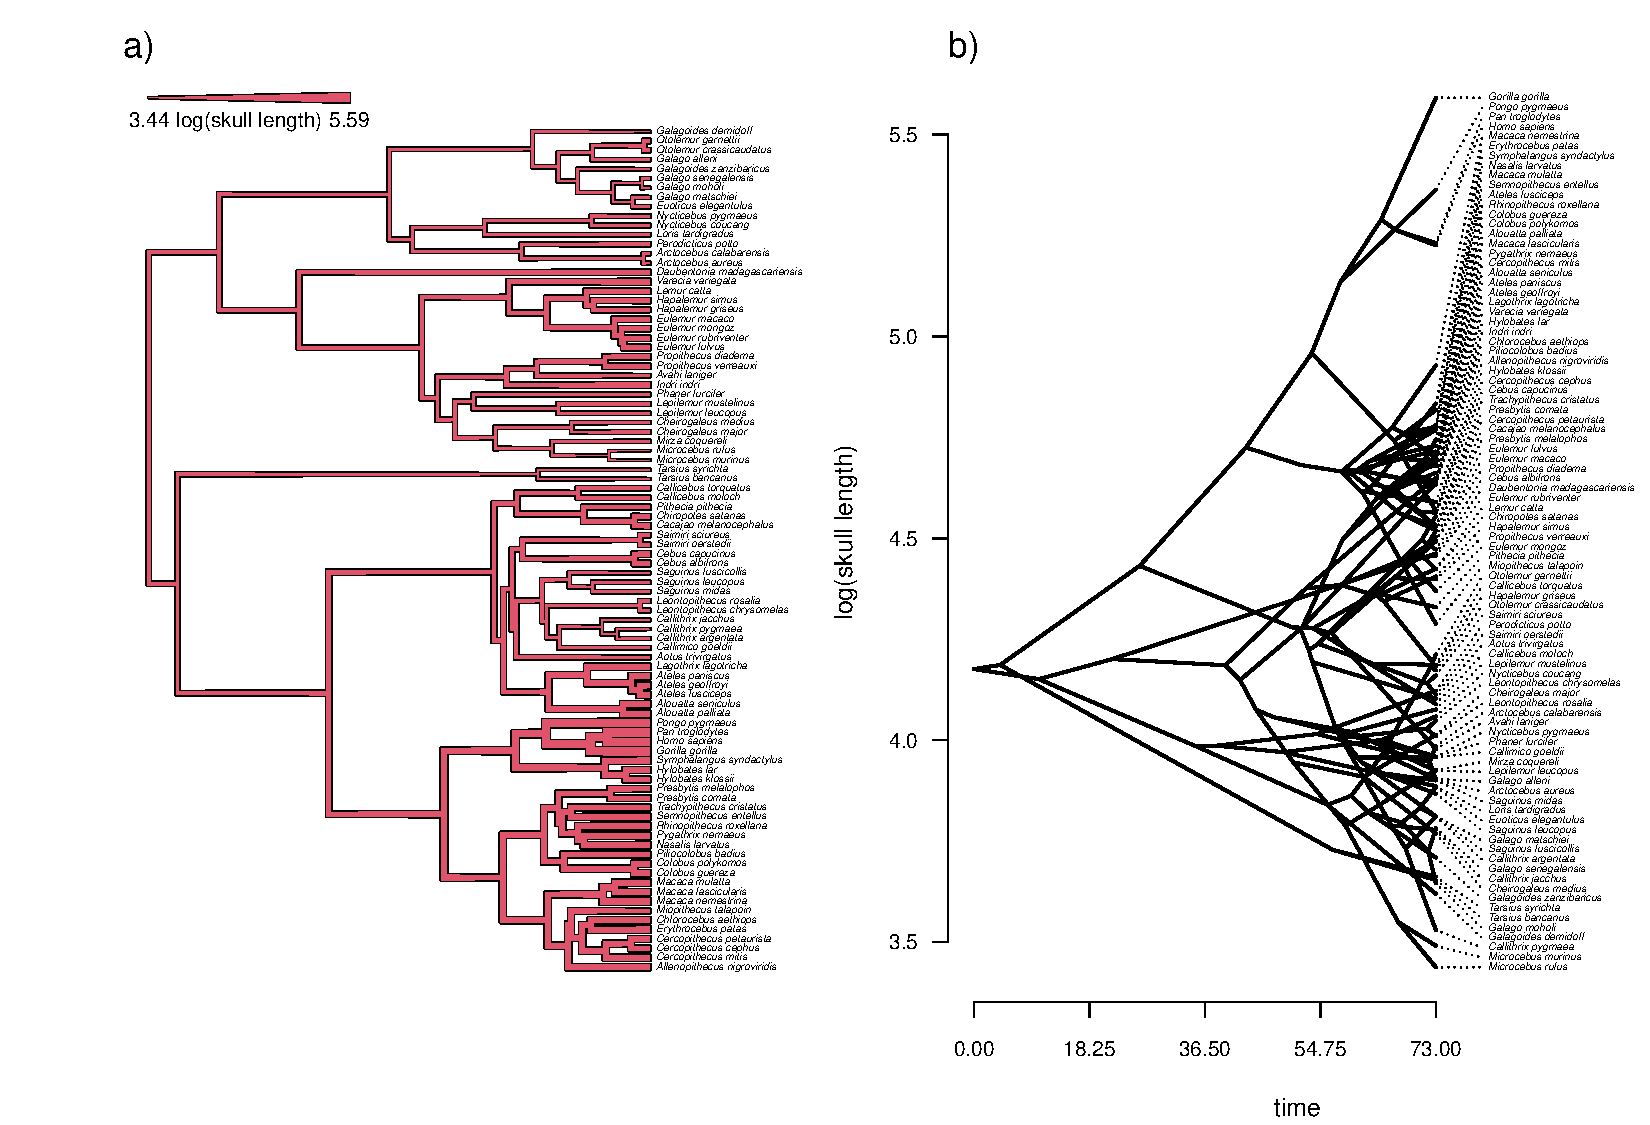
\includegraphics[width=1\linewidth]{old.Revell.phytools-v2_peerj_files/figure-latex/primate-edgewidth-1} %%%
\DIFdelendFL \DIFaddbeginFL 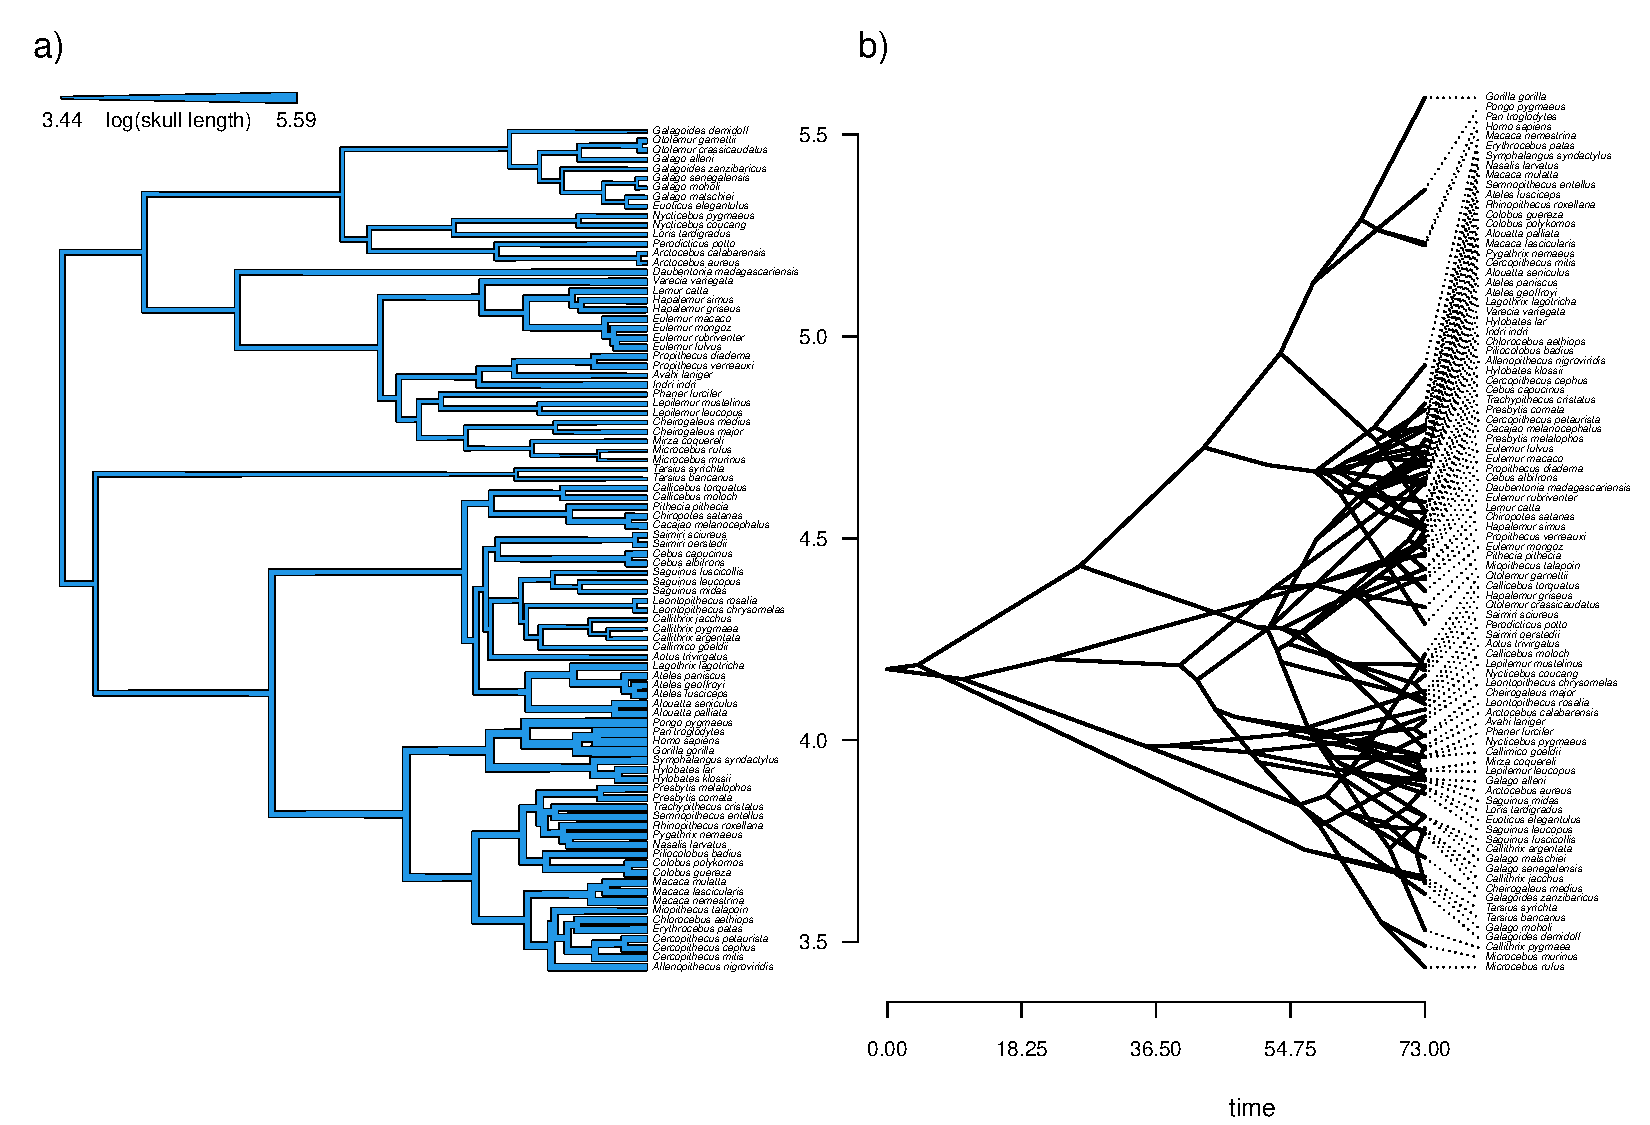
\includegraphics[width=1\linewidth]{Revell.phytools-v2_peerj_files/figure-latex/primate-edgewidth-1} \DIFaddendFL \caption{a) Primate skull lengths (on a log scale) projected onto the edges and nodes of the phylogeny. The width of each edge of the tree is proportional to the observed or reconstructed value of the trait. See main text for more details. b) A projection of the phylogeny of a) into a space defined by time since the root (on the horizontal axis) and log skull length. \DIFaddbeginFL \DIFaddFL{Phylogeny and data are derived from Kirk and Kay (2004). See main text for more details.}\DIFaddendFL }\label{fig:primate-edgewidth}
\end{figure}

\DIFdelbegin \DIFdel{Visual inspection of Figure @ref(fig:primate-edgewidth) may give us a
preliminary sense of where in our tree our penalized likelihood method
could end up showing the rate of primate skull length evolution to vary
the most -- and the least.
}%DIFDELCMD < 

%DIFDELCMD < %%%
\DIFdelend The function we'll use to fit our rate-variable model,
\texttt{multirateBM}, performs a computationally intensive optimization.
Setting the optional argument \texttt{parallel=TRUE} will help
distribute this burden across multiple processors of our computer, if
possible. \DIFdelbegin %DIFDELCMD < 

%DIFDELCMD < %%%
\DIFdelend Let's start \DIFdelbegin \DIFdel{with }\DIFdelend \DIFaddbegin \DIFadd{our analysis using a smoothing parameter,
}\DIFaddend \(\lambda\)\DIFaddbegin \DIFadd{, equal to \(\lambda\) }\DIFaddend = 1.0.

\begin{Shaded}
\begin{Highlighting}[]
\NormalTok{primate.mBM\_1}\OtherTok{\textless{}{-}}\FunctionTok{multirateBM}\NormalTok{(primate.tree,}
\NormalTok{  primate.lnSkull,}\DIFdelbegin \DIFdel{\AttributeTok{lamba=}}\DIFdelend \DIFaddbegin \DIFadd{\AttributeTok{lambda=}}\DIFaddend \DecValTok{1}\NormalTok{,}\AttributeTok{parallel=}\ConstantTok{TRUE}\NormalTok{)}
\end{Highlighting}
\end{Shaded}

\begin{verbatim}
## Beginning optimization....
## Using socket cluster with 16 nodes on host 'localhost'.
## Optimization iteration 1. Using "L-BFGS-B" (parallel) 
## optimization method.
## Best (penalized) log-likelihood so far: -267.108 
## Done optimization.
\end{verbatim}

Now we can do the same with \(\lambda\) = 0.1 and 10. \DIFaddbegin \DIFadd{Readers should
take special care to note that the specific values of the penalized log
likelihoods are not comparable between analyses with different values of
the penalty coefficient, \(\lambda\)! }\DIFaddend This time I'll turn off printing
by updating the optional argument to \texttt{quiet=TRUE}.

\begin{Shaded}
\begin{Highlighting}[]
\NormalTok{primate.mBM\_0}\FloatTok{.1}\OtherTok{\textless{}{-}}\FunctionTok{multirateBM}\NormalTok{(primate.tree,}
\NormalTok{  primate.lnSkull,}\AttributeTok{lambda=}\FloatTok{0.1}\NormalTok{,}\AttributeTok{parallel=}\ConstantTok{TRUE}\NormalTok{,}\AttributeTok{quiet=}\ConstantTok{TRUE}\NormalTok{)}
\NormalTok{primate.mBM\_10}\OtherTok{\textless{}{-}}\FunctionTok{multirateBM}\NormalTok{(primate.tree,}
\NormalTok{  primate.lnSkull,}\AttributeTok{lambda=}\DecValTok{10}\NormalTok{,}\AttributeTok{parallel=}\ConstantTok{TRUE}\NormalTok{,}\AttributeTok{quiet=}\ConstantTok{TRUE}\NormalTok{)}
\end{Highlighting}
\end{Shaded}

\DIFdelbegin \DIFdel{(Readers should take special care to note that the specific values of
the penalized log likelihoods are not comparable between analyses with
different values of the penalty coefficient, \(\lambda\)!)
}%DIFDELCMD < 

%DIFDELCMD < %%%
\DIFdelend Finally, let's visualize the differences and similarities between each
of our three fitted models.

\begin{Shaded}
\begin{Highlighting}[]
\FunctionTok{par}\NormalTok{(}\AttributeTok{mfrow=}\FunctionTok{c}\NormalTok{(}\DecValTok{1}\NormalTok{,}\DecValTok{3}\NormalTok{))}
\FunctionTok{plot}\NormalTok{(primate.mBM\_1,}\AttributeTok{ftype=}\StringTok{"off"}\NormalTok{,}\AttributeTok{lwd=}\DecValTok{2}\NormalTok{,}
  \AttributeTok{mar=}\FunctionTok{c}\NormalTok{(}\FloatTok{0.1}\NormalTok{,}\FloatTok{0.1}\NormalTok{,}\FloatTok{2.1}\NormalTok{,}\FloatTok{0.1}\NormalTok{))}
\FunctionTok{mtext}\NormalTok{(}\FunctionTok{expression}\NormalTok{(}\FunctionTok{paste}\NormalTok{(}\StringTok{"a) "}\NormalTok{,lambda,}\StringTok{" = 1"}\NormalTok{)),}\AttributeTok{adj=}\FloatTok{0.1}\NormalTok{,}
  \AttributeTok{line=}\FloatTok{0.5}\NormalTok{,}\AttributeTok{cex=}\FloatTok{1.1}\NormalTok{)}
\FunctionTok{plot}\NormalTok{(primate.mBM\_0}\FloatTok{.1}\NormalTok{,}\AttributeTok{ftype=}\StringTok{"off"}\NormalTok{,}\AttributeTok{lwd=}\DecValTok{2}\NormalTok{,}
  \AttributeTok{mar=}\FunctionTok{c}\NormalTok{(}\FloatTok{0.1}\NormalTok{,}\FloatTok{1.1}\NormalTok{,}\FloatTok{2.1}\NormalTok{,}\FloatTok{0.1}\NormalTok{))}
\FunctionTok{mtext}\NormalTok{(}\FunctionTok{expression}\NormalTok{(}\FunctionTok{paste}\NormalTok{(}\StringTok{"b) "}\NormalTok{,lambda,}\StringTok{" = 0.1"}\NormalTok{)),}\AttributeTok{adj=}\FloatTok{0.1}\NormalTok{,}
  \AttributeTok{line=}\FloatTok{0.5}\NormalTok{,}\AttributeTok{cex=}\FloatTok{1.1}\NormalTok{)}
\FunctionTok{plot}\NormalTok{(primate.mBM\_10,}\AttributeTok{ftype=}\StringTok{"off"}\NormalTok{,}\AttributeTok{lwd=}\DecValTok{2}\NormalTok{,}
  \AttributeTok{mar=}\FunctionTok{c}\NormalTok{(}\FloatTok{0.1}\NormalTok{,}\FloatTok{1.1}\NormalTok{,}\FloatTok{2.1}\NormalTok{,}\FloatTok{0.1}\NormalTok{))}
\FunctionTok{mtext}\NormalTok{(}\FunctionTok{expression}\NormalTok{(}\FunctionTok{paste}\NormalTok{(}\StringTok{"c) "}\NormalTok{,lambda,}\StringTok{" = 10"}\NormalTok{)),}\AttributeTok{adj=}\FloatTok{0.1}\NormalTok{,}
  \AttributeTok{line=}\FloatTok{0.5}\NormalTok{,}\AttributeTok{cex=}\FloatTok{1.1}\NormalTok{)}
\end{Highlighting}
\end{Shaded}

\begin{figure}
\DIFdelbeginFL %DIFDELCMD < \includegraphics[width=1\linewidth]{old.Revell.phytools-v2_peerj_files/figure-latex/multirateBM-1} %%%
\DIFdelendFL \DIFaddbeginFL \includegraphics[width=1\linewidth]{Revell.phytools-v2_peerj_files/figure-latex/multirateBM-1} \DIFaddendFL \caption{Estimated rates of log(skull length) evolution in primates under a variable-rate Brownian evolution model for different values of the smoothing parameter, $\lambda$. Increasing values of $\lambda$ should correspond to less variation in the rate of evolution across the tree. \DIFaddbeginFL \DIFaddFL{Phylogeny and data are based on Kirk and Kay (2004). }\DIFaddendFL See main text for additional details.}\label{fig:multirateBM}
\end{figure}

We can see from the plot of Figure @ref(fig:multirateBM) that even
though the specific range of rate variation depends strongly on our
specified values of \(\lambda\), the pattern from clade to clade on the
tree is relatively robust. This should give us some measure of
confidence that the our inferred rate heterogeneity may be a product of
real variability in the evolutionary rate for our character on the
phylogeny!

\hypertarget{diversification}{%
\section{Diversification}\label{diversification}}

In addition to the methods that we've seen so far, \emph{phytools} also
contains a handful of different techniques for investigating
diversification on reconstructed phylogenies. Diversification has never
been the primary focus of the \emph{phytools} R package (to that end,
I'd recommend the powerful \emph{diversitree} package, FitzJohn 2012),
but these methods are popular, and the \emph{phytools} implementations
can be relatively easy to use. \DIFaddbegin \DIFadd{Various additional R package include
interesting diversification models and methods, including }\emph{\DIFadd{hisse}}
\DIFadd{(Beaulieu and O'Meara 2016), }\emph{\DIFadd{RPANDA}} \DIFadd{(Morlon et al. 2016),
}\emph{\DIFadd{TreeSim}} \DIFadd{(Stadler 2019), }\emph{\DIFadd{DDD}} \DIFadd{(Etienne and Haegeman 2023),
and others.
}\DIFaddend 

\emph{phytools} contains methods to compute and visualize the
accumulation of lineages through time, including with extinction
(\texttt{ltt}), to calculate and test the \(\gamma\) statistic
(\texttt{gammatest}, \texttt{mccr}, Pybus and Harvey 2000), to fit
pure-birth and birth-death models, including with random missing taxa
(\texttt{fit.yule} and \texttt{fit.bd}, Nee et al. 1994; Stadler 2013),
to compare diversification rates between trees (\texttt{ratebytree},
Revell 2018), and to simulate stochastic trees under various conditions
(\texttt{pbtree}).

\hypertarget{lineage-through-time-plots}{%
\subsection{Lineage through time
plots}\label{lineage-through-time-plots}}

One of the most rudimentary phylogenetic methods for studying
diversification is to simply graph the accumulation of new lineages in
our reconstructed phylogeny over time since the global root of the tree.
This visualization method is called a lineage-through-time plot. \DIFdelbegin %DIFDELCMD < 

%DIFDELCMD < %%%
\DIFdel{One of the great
appeals }\DIFdelend \DIFaddbegin \DIFadd{A great
appeal }\DIFaddend of this visualization is that if we graph the number of lineages
through time in a fully-sampled pure-birth (that is, constant-rate
speciation, but no extinction) phylogenetic tree, the accumulation curve
should be exponential -- or exactly linear on a semi-logarithmic scale.
This means that the lineage-through-time plot gives us a handy tool that
we can use to compare the real lineage accumulation in our reconstructed
tree to this simple, neutral expectation (Pybus and Harvey 2000; Revell
and Harmon 2022).

To see how the number of lineages through time are calculated and
graphed using \emph{phytools}, let's load a phylogenetic tree of \DIFdelbegin \DIFdel{lizards
from the diverse South American family Liolaemidae}\DIFdelend \DIFaddbegin \DIFadd{snakes
from the venomous family Elapidae}\DIFaddend . This phylogeny is \DIFaddbegin \DIFadd{now }\DIFaddend packaged with
\emph{phytools} but \DIFdelbegin \DIFdel{was published by Esquerré }\DIFdelend \DIFaddbegin \DIFadd{derives from a study by Lee }\DIFaddend et al. (\DIFdelbegin \DIFdel{2019}\DIFdelend \DIFaddbegin \DIFadd{2016}\DIFaddend ).

\begin{Shaded}
\begin{Highlighting}[]
\FunctionTok{data}\DIFdelbegin \DIFdel{\NormalTok{(liolaemid.tree)}
\FunctionTok{print}\NormalTok{(liolaemid.tree,}}\DIFdelend \DIFaddbegin \DIFadd{\NormalTok{(elapidae.tree)}
\FunctionTok{print}\NormalTok{(elapidae.tree,}}\DIFaddend \AttributeTok{printlen=}\DecValTok{2}\NormalTok{)}
\end{Highlighting}
\end{Shaded}

\DIFmodbegin
\begin{DIFverbatim}[alsolanguage=DIFcode]
## 
%DIF < ## Phylogenetic tree with 257 tips and 256 internal nodes.
%DIF > ## Phylogenetic tree with 175 tips and 174 internal nodes.
## 
## Tip labels:
%DIF < ##   Liolaemus_abaucan, Liolaemus_koslowskyi, ...
%DIF > ##   Calliophis_bivirgata, Calliophis_melanurus, ...
## 
## Rooted; includes branch lengths.
\end{DIFverbatim}
\DIFmodend

We're going to create our lineage-through-time graph with
\emph{phytools} over two steps. \DIFdelbegin %DIFDELCMD < 

%DIFDELCMD < %%%
\DIFdelend First, we'll use the \emph{phytools}
function \texttt{ltt} to compute an object of class \texttt{"ltt"}
containing our tree and a count of the number of lineages through time
from the root of the tree to the tips.

\begin{Shaded}
\begin{Highlighting}[]
\DIFdelbegin \DIFdel{\NormalTok{liolaemid.ltt}\OtherTok{\textless{}{-}}\FunctionTok{ltt}\NormalTok{(liolaemid.tree,}}\DIFdelend \DIFaddbegin \DIFadd{\NormalTok{elapidae.ltt}\OtherTok{\textless{}{-}}\FunctionTok{ltt}\NormalTok{(elapidae.tree,}}\DIFaddend \AttributeTok{plot=}\ConstantTok{FALSE}\NormalTok{)}
\DIFdelbegin \DIFdel{\NormalTok{liolaemid.ltt}
}\DIFdelend \DIFaddbegin \DIFadd{\NormalTok{elapidae.ltt}
}\DIFaddend \end{Highlighting}
\end{Shaded}

\DIFmodbegin
\begin{DIFverbatim}[alsolanguage=DIFcode]
## Object of class "ltt" containing:
## 
%DIF < ## (1) A phylogenetic tree with 257 tips and 256 internal
%DIF > ## (1) A phylogenetic tree with 175 tips and 174 internal
##     nodes.
## 
## (2) Vectors containing the number of lineages (ltt) and
##     branching times (times) on the tree.
## 
## (3) A value for Pybus & Harvey's "gamma" statistic of
%DIF < ##     gamma = 1.8129, p-value = 0.0698.
%DIF > ##     gamma = -3.3244, p-value = 0.0009.
\end{DIFverbatim}
\DIFmodend

From the print-out we see that in addition to the tree and the lineages
through time, our object also contains a value of (and a P-value for)
Pybus and Harvey's (2000) \(\gamma\) statistic. \DIFdelbegin %DIFDELCMD < 

%DIFDELCMD < %%%
\DIFdelend \(\gamma\) is a
numerical value used to describe the general shape of the lineage
through time curve. If the curve is straight (on a semi-log scale), then
\(\gamma\) should have a value close to zero. This is what we expect
under a pure-birth (speciation only) diversification process. On the
other hand, significantly positive or significantly negative \(\gamma\)
mean that the lineage through time graph curves upward or downward
towards the present day (Pybus and Harvey 2000). \DIFdelbegin \DIFdel{This could
}\DIFdelend \DIFaddbegin \DIFadd{Significant positive or
negative curvature of the lineage-through-time plot might }\DIFaddend mean that the
rate of diversification has changed over time, but it could also be due
to past extinction or incomplete taxon sampling (Revell and Harmon
2022). \DIFdelbegin %DIFDELCMD < 

%DIFDELCMD < %%%
\DIFdel{We can see that for our liolaemid lizards, }\DIFdelend \DIFaddbegin \DIFadd{Note that since the pull of the present (Nee et al. 1992) means
that our lineage through time plot is expected to curve upwards towards
the present day for any non-zero rate of extinction, some have argued
that }\DIFaddend \(\gamma\) \DIFdelbegin \DIFdel{is slightly
}\DIFdelend \DIFaddbegin \DIFadd{should only be interpreted when }\DIFaddend \emph{\DIFdelbegin \DIFdel{positive}%DIFDELCMD < \MBLOCKRIGHTBRACE%%%
\DIFdel{,
though not significantly so}\DIFdelend \DIFaddbegin \DIFadd{negative}}\DIFadd{. (I.e.,
that statistical tests of \(\gamma\) are properly one-tailed.) I don't
subscribe to that view, inasmuch as I see \(\gamma\) as a
phenomenological measure of lineage accumulation in our reconstructed
tree whose positive or negative deviation from the statistic's expected
value under pure-birth could have multiple underlying causes. At first
look, the value of \(\gamma\) from our elapid snake phylogeny would seem
to be highly significantly }\emph{\DIFadd{negative}}\DIFaddend .

\DIFaddbegin \DIFadd{To proceed and graph our object created in the previous step, we merely
need to execute a generic }\texttt{\DIFadd{plot}} \DIFadd{method function call as follows.
A simple }\texttt{\DIFadd{plot}} \DIFadd{call would have done the trick; however, in this
case I decided to first leave off the axes of my plot, and then re-plot
them so that I could make our horizontal (}\emph{\DIFadd{x}}\DIFadd{) axis run
}\emph{\DIFadd{backwards}} \DIFadd{in time (i.e., right to left) from the present day into
the past. I've also super-imposed the phylogeny itself on our plot so
that we can more easily visualization the relationship between the
structure of our phylogenetic tree and the accumulation of lineages over
time.
}

\DIFaddend \begin{Shaded}
\begin{Highlighting}[]
\FunctionTok{par}\NormalTok{(}\AttributeTok{mar=}\FunctionTok{c}\NormalTok{(}\FloatTok{5.1}\NormalTok{,}\FloatTok{4.1}\NormalTok{,}\FloatTok{1.1}\NormalTok{,}\FloatTok{2.1}\NormalTok{))}
\FunctionTok{plot}\DIFdelbegin \DIFdel{\NormalTok{(liolaemid.ltt,}}\DIFdelend \DIFaddbegin \DIFadd{\NormalTok{(elapidae.ltt,}}\DIFaddend \AttributeTok{show.tree=}\ConstantTok{TRUE}\NormalTok{,}\AttributeTok{lwd=}\DecValTok{2}\NormalTok{,}
  \AttributeTok{log.lineages=}\ConstantTok{FALSE}\NormalTok{,}\AttributeTok{log=}\StringTok{"y"}\NormalTok{,}\AttributeTok{bty=}\StringTok{"n"}\NormalTok{,}\DIFaddbegin \DIFadd{\AttributeTok{cex.lab=}\FloatTok{0.9}\NormalTok{,}
  \AttributeTok{transparency=}\FloatTok{0.1}\NormalTok{,}\AttributeTok{axes=}\ConstantTok{FALSE}\NormalTok{,}
  \AttributeTok{xlab=}\StringTok{"millions of year bp"}\NormalTok{)}
\NormalTok{h}\OtherTok{\textless{}{-}}\FunctionTok{max}\NormalTok{(}\FunctionTok{nodeHeights}\NormalTok{(elapidae.tree))}
\FunctionTok{axis}\NormalTok{(}\DecValTok{1}\NormalTok{,}\AttributeTok{at=}\NormalTok{h}\SpecialCharTok{{-}}\FunctionTok{seq}\NormalTok{(}\DecValTok{0}\NormalTok{,}\DecValTok{35}\NormalTok{,}\AttributeTok{by=}\DecValTok{5}\NormalTok{),}\AttributeTok{labels=}\FunctionTok{seq}\NormalTok{(}\DecValTok{0}\NormalTok{,}\DecValTok{35}\NormalTok{,}\AttributeTok{by=}\DecValTok{5}\NormalTok{),}}\DIFaddend \AttributeTok{las=}\DecValTok{1}\NormalTok{,}
  \AttributeTok{cex.axis=}\FloatTok{0.8}\DIFdelbegin \DIFdel{\NormalTok{,}\AttributeTok{cex.lab=}\FloatTok{0.9}\NormalTok{,}\AttributeTok{transparency=}\FloatTok{0.1}}\DIFdelend \DIFaddbegin \DIFadd{\NormalTok{)}
\FunctionTok{axis}\NormalTok{(}\DecValTok{2}\NormalTok{,}\AttributeTok{las=}\DecValTok{1}\NormalTok{,}\AttributeTok{cex.axis=}\FloatTok{0.8}}\DIFaddend \NormalTok{)}
\end{Highlighting}
\end{Shaded}

\begin{figure}
\DIFdelbeginFL %DIFDELCMD < 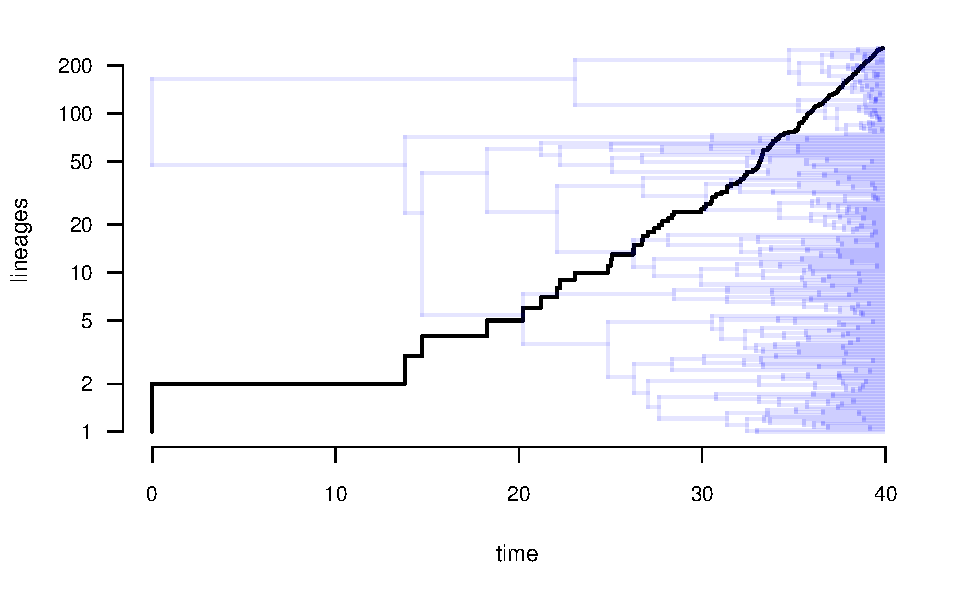
\includegraphics[width=1\linewidth]{old.Revell.phytools-v2_peerj_files/figure-latex/liol-ltt-1} %%%
\DIFdelendFL \DIFaddbeginFL 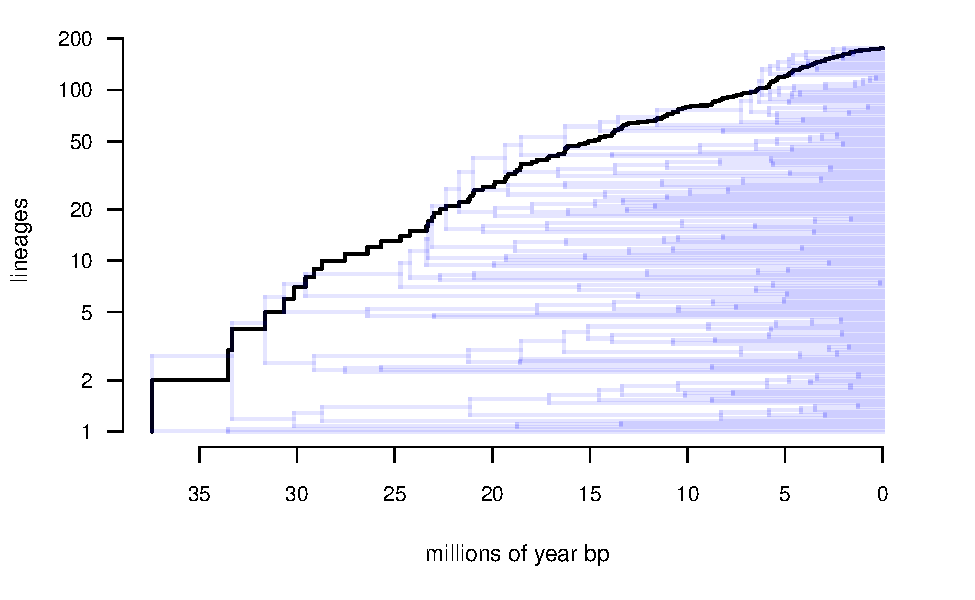
\includegraphics[width=1\linewidth]{Revell.phytools-v2_peerj_files/figure-latex/elap-ltt-1} \DIFaddendFL \caption{Lineage through time plot for phylogeny of \DIFdelbeginFL \DIFdelFL{lizards }\DIFdelendFL \DIFaddbeginFL \DIFaddFL{snakes }\DIFaddendFL from the \DIFdelbeginFL \DIFdelFL{South American }\DIFdelendFL family \DIFdelbeginFL \DIFdelFL{Liolaemidae}\DIFdelendFL \DIFaddbeginFL \DIFaddFL{Elapidae (Lee et al}\DIFaddendFL . \DIFaddbeginFL \DIFaddFL{2016). }\DIFaddendFL See main text for more details.}\DIFdelbeginFL %DIFDELCMD < \label{fig:liol-ltt}
%DIFDELCMD < %%%
\DIFdelendFL \DIFaddbeginFL \label{fig:elap-ltt}
\DIFaddendFL \end{figure}

In general, accounting for incomplete taxon sampling in the measurement
of the \(\gamma\) statistic is important because missing taxa will tend
to pull our lineage-through-time curve downwards as we approach the tips
of the tree -- in other words, towards more negative values of
\(\gamma\)\DIFaddbegin \DIFadd{, just like the value that we see for our lineage through time
plot of Figure @ref(fig:elap-ltt)}\DIFaddend .

Fortunately, there's a simple way to address this bias. If we know the
\DIFdelbegin \DIFdel{true }\DIFdelend \DIFaddbegin \emph{\DIFadd{true}} \DIFaddend species richness of our clade of interest, we can simply
simulate trees that match this richness under pure-birth, randomly prune
taxa to the level of ``missingness'' in our reconstructed tree, and then
use the distribution of \(\gamma\) values across this set of simulated
(and then randomly pruned) trees as our null distribution for hypothesis
testing! This exact procedure is called the ``Monte Carlo constant
rates'' (\DIFdelbegin \DIFdel{or
}\DIFdelend MCCR, Pybus and Harvey 2000) test and is implemented in the
\emph{phytools} function \texttt{mccr}.

Of course, since the MCCR test accounts for randomly missing taxa from
our tree, we must know or hypothesize a true species richness of our
clade. In this instance, we're not too preoccupied about the precise
value for \DIFdelbegin \DIFdel{Liolaemidae, but the }\emph{\DIFdel{Reptile Database}} %DIFAUXCMD
\DIFdel{puts the species
richness of this diverse South American family at 340. For }\DIFdelend \DIFaddbegin \DIFadd{Elapidae, but Lee et al. (2016) purported that their phylogeny
included approximately 50\% of know elapids at the time. Even though
it's likely that elapid diversity has changed a bit in the intervening
years, for }\DIFaddend illustrative purposes only, let's just go with this \DIFdelbegin \DIFdel{number! }\DIFdelend \DIFaddbegin \DIFadd{50\%
figure! In both }\texttt{\DIFadd{mccr}} \DIFadd{and the birth-death model-fitting function
we'll use later, sampling fraction is specified via the argument
}\texttt{\DIFadd{rho}} \DIFadd{(for the Greek letter \(\rho\)).
}\DIFaddend 

\begin{Shaded}
\begin{Highlighting}[]
\DIFdelbegin \DIFdel{\NormalTok{liolaemid.mccr}\OtherTok{\textless{}{-}}\FunctionTok{mccr}\NormalTok{(liolaemid.ltt,}
  \AttributeTok{rho=}\FunctionTok{Ntip}\NormalTok{(liolaemid.tree)}\SpecialCharTok{/}\DecValTok{340}}\DIFdelend \DIFaddbegin \DIFadd{\NormalTok{elapidae.mccr}\OtherTok{\textless{}{-}}\FunctionTok{mccr}\NormalTok{(elapidae.ltt,}\AttributeTok{rho=}\FloatTok{0.5}}\DIFaddend \NormalTok{,}\AttributeTok{nsim=}\DecValTok{1000}\NormalTok{)}
\DIFdelbegin \DIFdel{\NormalTok{liolaemid.mccr}
}\DIFdelend \DIFaddbegin \DIFadd{\NormalTok{elapidae.mccr}
}\DIFaddend \end{Highlighting}
\end{Shaded}

\DIFmodbegin
\begin{DIFverbatim}[alsolanguage=DIFcode]
## Object of class "mccr" consisting of:
## 
## (1) A value for Pybus & Harvey's "gamma" statistic of 
%DIF < ##     gamma = 1.8129.
%DIF > ##     gamma = -3.3244.
## 
%DIF < ## (2) A two-tailed p-value from the MCCR test of 0.002.
%DIF > ## (2) A two-tailed p-value from the MCCR test of 0.446.
## 
## (3) A simulated null-distribution of gamma from 1000
##     simulations.
\end{DIFverbatim}
\DIFmodend

This tells us that, having accounted for missing taxa, our observed
value of \(\gamma\) \DIFdelbegin \DIFdel{becomes highly significantly different from that
expected }\DIFdelend \DIFaddbegin \DIFadd{(previously highly significantly negative) becomes
indistinguishable from what we'd expect }\DIFaddend under pure-birth. We can plot
our results to see what I mean.

\begin{Shaded}
\begin{Highlighting}[]
\FunctionTok{par}\NormalTok{(}\AttributeTok{mar=}\FunctionTok{c}\NormalTok{(}\FloatTok{5.1}\NormalTok{,}\FloatTok{4.1}\NormalTok{,}\FloatTok{0.6}\NormalTok{,}\FloatTok{2.1}\NormalTok{))}
\FunctionTok{plot}\DIFdelbegin \DIFdel{\NormalTok{(liolaemid.mccr,}}\DIFdelend \DIFaddbegin \DIFadd{\NormalTok{(elapidae.mccr,}}\DIFaddend \AttributeTok{las=}\DecValTok{1}\NormalTok{,}\AttributeTok{cex.lab=}\FloatTok{0.8}\NormalTok{,}\AttributeTok{cex.axis=}\FloatTok{0.7}\NormalTok{,}
  \AttributeTok{main=}\StringTok{""}\NormalTok{)}
\end{Highlighting}
\end{Shaded}

\begin{figure}
\DIFdelbeginFL %DIFDELCMD < 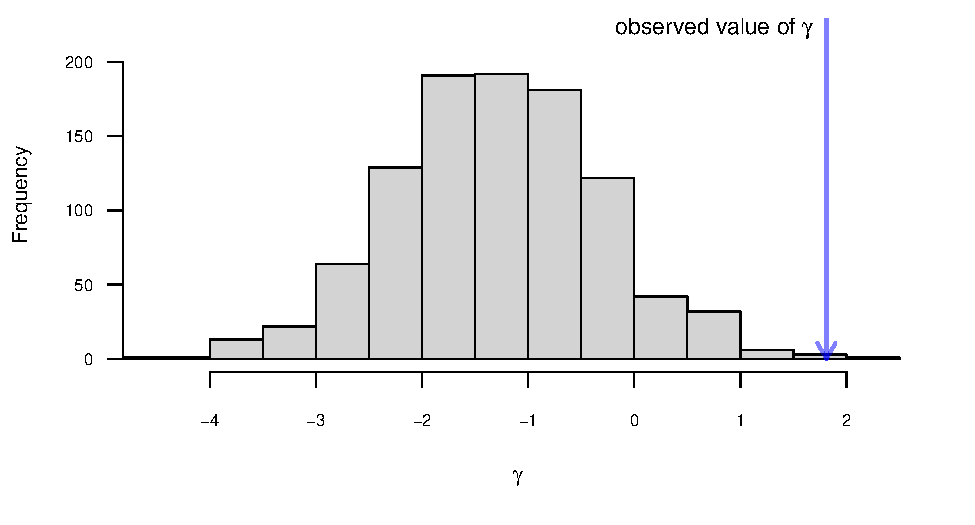
\includegraphics[width=1\linewidth]{old.Revell.phytools-v2_peerj_files/figure-latex/liol-mccr-1} %%%
\DIFdelendFL \DIFaddbeginFL 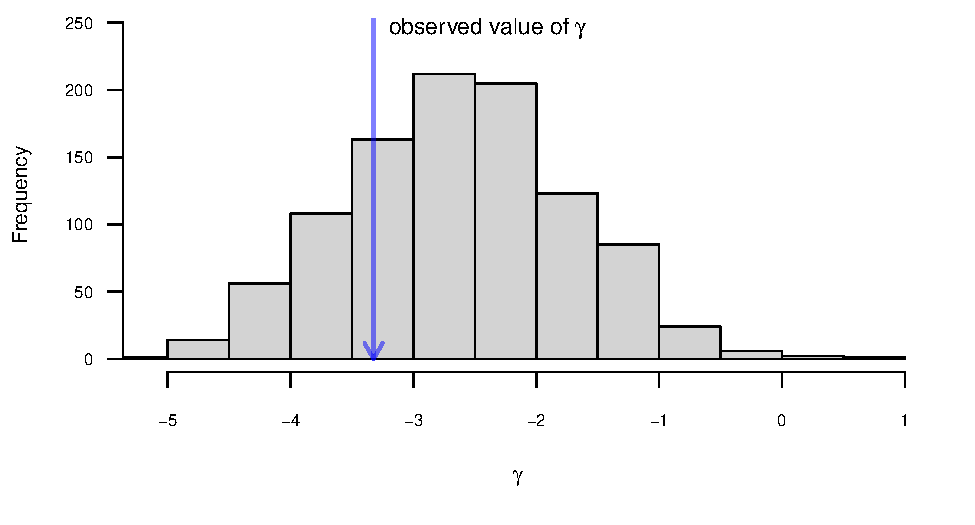
\includegraphics[width=1\linewidth]{Revell.phytools-v2_peerj_files/figure-latex/liol-mccr-1} \DIFaddendFL \caption{\DIFdelbeginFL \DIFdelFL{Lineage }\DIFdelendFL \DIFaddbeginFL \DIFaddFL{Distribution of simulated values of $\gamma$ for the MCCR test, and observed value for the lineage }\DIFaddendFL through time \DIFdelbeginFL \DIFdelFL{plot for phylogeny }\DIFdelendFL \DIFaddbeginFL \DIFaddFL{curve }\DIFaddendFL of \DIFdelbeginFL \DIFdelFL{lizards from }\DIFdelendFL the \DIFdelbeginFL \DIFdelFL{South American family Liolaemidae}\DIFdelendFL \DIFaddbeginFL \DIFaddFL{phylogeny of elapid snakes given in Figure 15. Phylogenetic tree based on Lee et al}\DIFaddendFL . \DIFaddbeginFL \DIFaddFL{(2016). See main text for more details.}\DIFaddendFL }\label{fig:liol-mccr}
\end{figure}

Figure @ref(fig:liol-mccr) shows that the measured value of \(\gamma\)
by \DIFdelbegin \DIFdel{this test is strongly significantly positive -- in other words
(accounting for missing taxa) , much larger than expected by random
chance under a constant-rate pure birth speciation process!
}\DIFdelend \DIFaddbegin \DIFadd{the MCCR test is no longer significant, demonstrating the vital
importance of accounting for incomplete taxon sampling in this (and
other) diversification analyses using phylogenies.
}\DIFaddend 

\hypertarget{modeling-speciation-and-extinction}{%
\subsection{Modeling speciation and
extinction}\label{modeling-speciation-and-extinction}}

In addition to these analysis, \emph{phytools} can also fit simple
speciation and extinction models following Nee et al. (1994; Stadler
2013; Harmon 2019). This is done primarily using the function
\texttt{fit.bd}, which also allows us to take into account an incomplete
taxonomic sampling fraction (Stadler 2013).

Just as with \(\gamma\), incomplete sampling has the potentially to
substantially distort our estimated rates of speciation (normally given
as \(\lambda\) -- a different \(\lambda\) from before!) and extinction
(\(\mu\)). In this case, ignoring (or underestimating) the missing
lineages in our tree will tend to cause us to underestimate the rate of
extinction, as nearly all of the information we have about extinction
comes from the most recent parts of our phylogeny! (See \DIFaddbegin \DIFadd{Stadler 2013;
}\DIFaddend Harmon 2019; Revell and Harmon 2022 for more details.)

Fitting a birth-death model using \emph{phytools} is very easy. \DIFaddbegin \DIFadd{For this
example, we'll use phylogenetic tree of lizards from the diverse South
American family Liolaemidae. Just as in the other examples this
phylogeny is packaged with }\emph{\DIFadd{phytools}}\DIFadd{, but was originally published
by Esquerré et al. (2019). (This is the same phylogeny that was used to
study the evolution of parity mode evolution under the hidden rates
model in an earlier section.)
}

\begin{Shaded}
\begin{Highlighting}[]
\DIFadd{\FunctionTok{data}\NormalTok{(liolaemid.tree)}
\FunctionTok{print}\NormalTok{(liolaemid.tree,}\AttributeTok{printlen=}\DecValTok{2}\NormalTok{)}
}\end{Highlighting}
\end{Shaded}

\DIFmodbegin
\begin{DIFverbatim}[alsolanguage=DIFcode]
%DIF > ## 
%DIF > ## Phylogenetic tree with 257 tips and 256 internal nodes.
%DIF > ## 
%DIF > ## Tip labels:
%DIF > ##   Liolaemus_abaucan, Liolaemus_koslowskyi, ...
%DIF > ## 
%DIF > ## Rooted; includes branch lengths.
\end{DIFverbatim}
\DIFmodend

\DIFaddend We'll pass our liolaemid tree to the \texttt{fit.bd} function, and the
only additional argument to be assigned is \texttt{rho} (for \(\rho\)),
the sampling fraction, \DIFdelbegin \DIFdel{which we 'll set }\DIFdelend \DIFaddbegin \DIFadd{just as we did for the MCCR test in the function
}\texttt{\DIFadd{mccr}}\DIFadd{. The }\emph{\DIFadd{Reptile Database}} \DIFadd{(Uetz et al. 2023) puts the
total species richness of Liolaemidae at 341, so we can set }\texttt{\DIFadd{rho}}
\DIFaddend to have a value equal to the number of tips in our tree divided by \DIFdelbegin \DIFdel{the quantity(340, see above) that we
hypothesize represents the true species richness of Liolaemidae}\DIFdelend \DIFaddbegin \DIFadd{this
quantity}\DIFaddend .

\begin{Shaded}
\begin{Highlighting}[]
\DIFaddbegin \DIFadd{\NormalTok{liolaemid.rho}\OtherTok{\textless{}{-}}\FunctionTok{Ntip}\NormalTok{(liolaemid.tree)}\SpecialCharTok{/}\DecValTok{341}
}\DIFaddend \NormalTok{liolaemid.bd}\OtherTok{\textless{}{-}}\FunctionTok{fit.bd}\NormalTok{(liolaemid.tree,}\AttributeTok{rho=}\DIFdelbegin \DIFdel{\FunctionTok{Ntip}\NormalTok{(liolaemid.tree)}\SpecialCharTok{/}\DecValTok{340}\NormalTok{)}
}\DIFdelend \DIFaddbegin \DIFadd{\NormalTok{liolaemid.rho)}
}\DIFaddend \NormalTok{liolaemid.bd}
\end{Highlighting}
\end{Shaded}

\DIFmodbegin
\begin{DIFverbatim}[alsolanguage=DIFcode]
## 
## Fitted birth-death model:
## 
%DIF < ## ML(b/lambda) = 0.351 
%DIF < ## ML(d/mu) = 0.1771 
%DIF > ## ML(b/lambda) = 0.352 
%DIF > ## ML(d/mu) = 0.1781 
## log(L) = 526.451 
## 
%DIF < ## Assumed sampling fraction (rho) = 0.7559 
%DIF > ## Assumed sampling fraction (rho) = 0.7537 
## 
## R thinks it has converged.
\end{DIFverbatim}
\DIFmodend

Other R packages (such as the aforementioned \emph{diversitree}) might
allow us to compare our fitted birth-death model to a range of other
hypotheses about diversification, such as that the speciation and
extinction rates change through time or as a function of our phenotypic
traits (e.g., Maddison et al. 2007; FitzJohn 2010; Morlon et al. 2010;
Revell and Harmon 2022). In \emph{phytools} we can compare our fitted
birth-death model to only one alternative model: the simpler, pure-birth
model -- also called a `Yule' model.

\begin{Shaded}
\begin{Highlighting}[]
\NormalTok{liolaemid.yule}\OtherTok{\textless{}{-}}\FunctionTok{fit.yule}\NormalTok{(liolaemid.tree,}
  \AttributeTok{rho=}\DIFdelbegin \DIFdel{\FunctionTok{Ntip}\NormalTok{(liolaemid.tree)}\SpecialCharTok{/}\DecValTok{340}\NormalTok{)}
}\DIFdelend \DIFaddbegin \DIFadd{\NormalTok{liolaemid.rho)}
}\DIFaddend \NormalTok{liolaemid.yule}
\end{Highlighting}
\end{Shaded}

\DIFmodbegin
\begin{DIFverbatim}[alsolanguage=DIFcode]
## 
## Fitted Yule model:
## 
%DIF < ## ML(b/lambda) = 0.2499 
%DIF < ## log(L) = 521.2295 
%DIF > ## ML(b/lambda) = 0.2502 
%DIF > ## log(L) = 521.1832 
## 
%DIF < ## Assumed sampling fraction (rho) = 0.7559 
%DIF > ## Assumed sampling fraction (rho) = 0.7537 
## 
## R thinks it has converged.
\end{DIFverbatim}
\DIFmodend

\begin{Shaded}
\begin{Highlighting}[]
\FunctionTok{anova}\NormalTok{(liolaemid.yule,liolaemid.bd)}
\end{Highlighting}
\end{Shaded}

\DIFmodbegin
\begin{DIFverbatim}[alsolanguage=DIFcode]
##                  log(L) d.f.       AIC     weight
%DIF < ## liolaemid.yule 521.2295    1 -1040.459 0.0144644
%DIF < ## liolaemid.bd   526.4510    2 -1048.902 0.9855356
%DIF > ## liolaemid.yule 521.1832    1 -1040.366 0.01381943
%DIF > ## liolaemid.bd   526.4510    2 -1048.902 0.98618057
\end{DIFverbatim}
\DIFmodend

This result tells us that, in the context of the two very simple models
that we've fit to our reconstructed tree, a two-parameter birth-death
(speciation and extinction) model is much better supported than our
simpler Yule model!

Lastly, the \emph{phytools} function \texttt{fit.bd} exports a
likelihood function as part of the fitted model object. This, in turn,
makes it very straightforward for \emph{phytools} users to (for example)
compute and graph the likelihood surface. Here, I'll illustrate this
using the base R graphics function \texttt{persp}. (But R and
contributed R packages contain lots of even fancier 3D plotting methods
that readers might be more interested in trying!)

\begin{Shaded}
\begin{Highlighting}[]
\NormalTok{ngrid}\OtherTok{\textless{}{-}}\DecValTok{40}
\NormalTok{b}\OtherTok{\textless{}{-}}\FunctionTok{seq}\NormalTok{(}\FloatTok{0.25}\NormalTok{,}\FloatTok{0.45}\NormalTok{,}\AttributeTok{length.out=}\NormalTok{ngrid)}
\NormalTok{d}\OtherTok{\textless{}{-}}\FunctionTok{seq}\NormalTok{(}\FloatTok{0.10}\NormalTok{,}\FloatTok{0.25}\NormalTok{,}\AttributeTok{length.out=}\NormalTok{ngrid)}
\NormalTok{logL}\OtherTok{\textless{}{-}}\FunctionTok{matrix}\NormalTok{(}\ConstantTok{NA}\NormalTok{,ngrid,ngrid)}
\ControlFlowTok{for}\NormalTok{(i }\ControlFlowTok{in} \DecValTok{1}\SpecialCharTok{:}\NormalTok{ngrid) }\ControlFlowTok{for}\NormalTok{(j }\ControlFlowTok{in} \DecValTok{1}\SpecialCharTok{:}\NormalTok{ngrid)}
\NormalTok{  logL[i,j]}\OtherTok{\textless{}{-}}\NormalTok{liolaemid.bd}\SpecialCharTok{$}\FunctionTok{lik}\NormalTok{(}\FunctionTok{c}\NormalTok{(b[i],d[j]))}
\NormalTok{logL[}\FunctionTok{is.nan}\NormalTok{(logL)]}\OtherTok{\textless{}{-}}\FunctionTok{min}\NormalTok{(logL[}\SpecialCharTok{!}\FunctionTok{is.nan}\NormalTok{(logL)])}
\FunctionTok{par}\NormalTok{(}\AttributeTok{mar=}\FunctionTok{rep}\NormalTok{(}\FloatTok{0.1}\NormalTok{,}\DecValTok{4}\NormalTok{))}
\FunctionTok{persp}\NormalTok{(b,d,}\FunctionTok{exp}\NormalTok{(logL),}\AttributeTok{shade=}\FloatTok{0.3}\NormalTok{,}\AttributeTok{phi=}\DecValTok{45}\NormalTok{,}\AttributeTok{theta=}\DecValTok{20}\NormalTok{,}
  \AttributeTok{xlab=}\StringTok{"speciation rate"}\NormalTok{,}\AttributeTok{ylab=}\StringTok{"extinction rate"}\NormalTok{,}
  \AttributeTok{zlab=}\StringTok{"likelihood"}\NormalTok{,}\AttributeTok{border=}\FunctionTok{palette}\NormalTok{()[}\DecValTok{4}\NormalTok{],}\AttributeTok{expand=}\FloatTok{0.3}\NormalTok{)}
\end{Highlighting}
\end{Shaded}

\begin{figure}
\DIFdelbeginFL %DIFDELCMD < 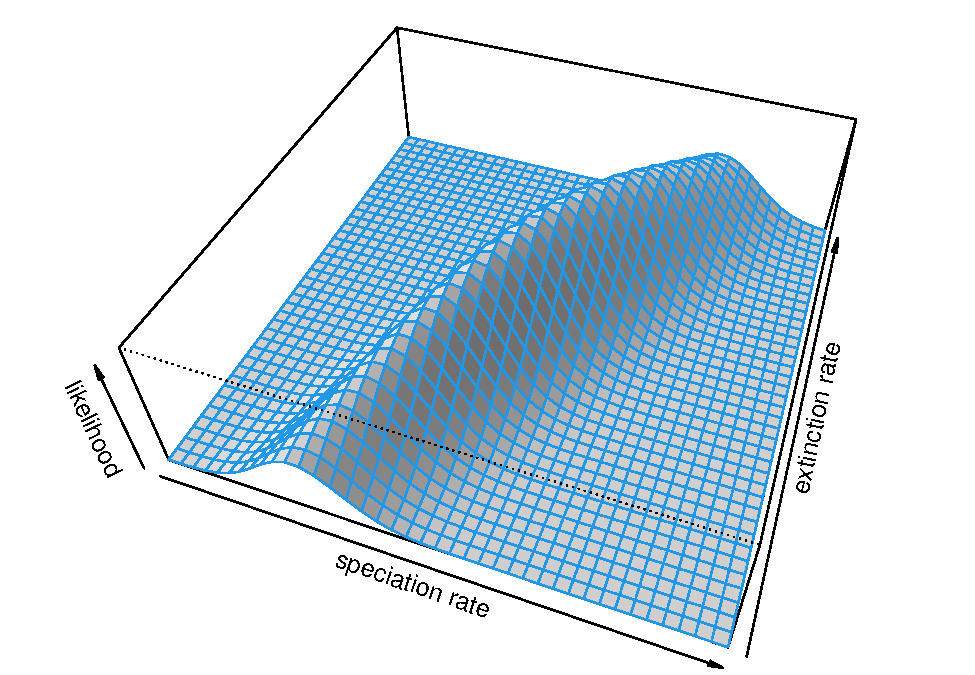
\includegraphics[width=1\linewidth]{old.Revell.phytools-v2_peerj_files/figure-latex/liol-bd-3d-1} %%%
\DIFdelendFL \DIFaddbeginFL 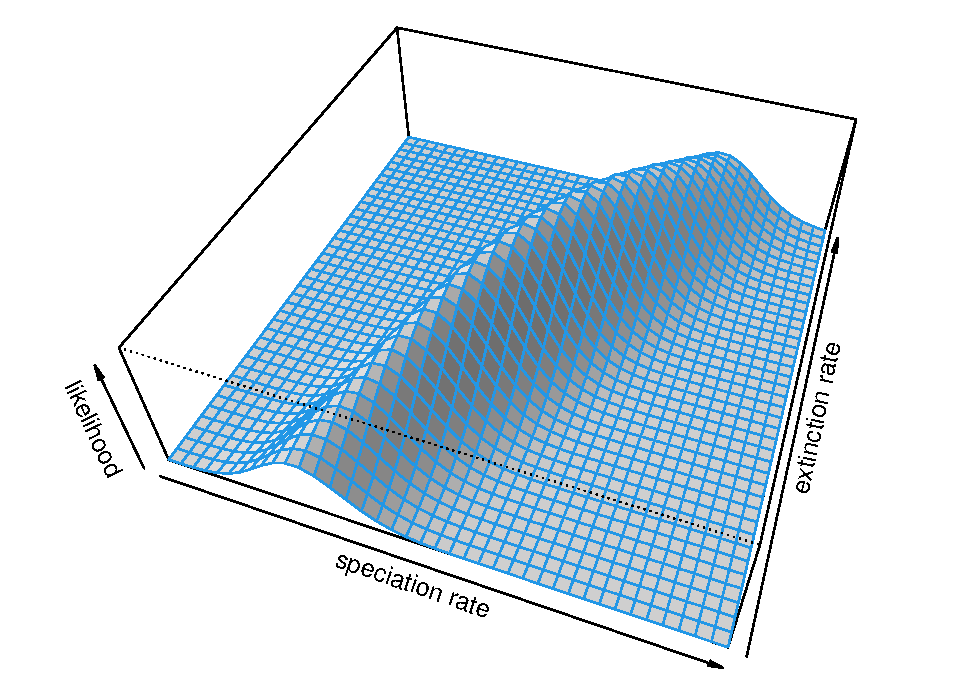
\includegraphics[width=1\linewidth]{Revell.phytools-v2_peerj_files/figure-latex/liol-bd-3d-1} \DIFaddendFL \caption{Visualization of the likelihood surface for speciation and extinction rates estimated for a phylogenetic tree of Liolaemidae. The ridge of values with similar likelihoods is typical of this class of model. \DIFaddbeginFL \DIFaddFL{Phylogenetic tree from Esquerr\'e et al. (2019). }\DIFaddendFL See main text for more details.}\label{fig:liol-bd-3d}
\end{figure}

\DIFdelbegin \DIFdel{(}\DIFdelend Some astute readers will notice the line \texttt{logL{[}is.nan(logL){]}}
\texttt{\textless{}-} \texttt{min(...)} (etc.) in my script of above.
This is because during our grid evaluation of the likelihood function,
sometimes the function was being evaluated in parameter space where the
likelihood is not defined. To account for this I set all parts of the
likelihood surface that could not be computed to the numerical minimum
of the graph!
\DIFdelbegin \DIFdel{)
}\DIFdelend 

Figure @ref(fig:liol-bd-3d) shows the very strong \emph{ridge} in the
likelihood surface (from low \(\lambda\) and low \(\mu\), to high
\(\lambda\) and high \(\mu\)) that almost invariably tends to
characterize the likelihood surfaces of birth-death models.

\hypertarget{visualization}{%
\section{Visualization}\label{visualization}}

After phylogenetic comparative analysis, \emph{phytools} is perhaps best
known for its phylogeny visualization methods\DIFdelbegin \DIFdel{.
}%DIFDELCMD < 

%DIFDELCMD < %%%
\DIFdel{We}\DIFdelend \DIFaddbegin \DIFadd{, and we}\DIFaddend 've seen a number
of these approaches already deployed throughout this article. For
example, in Figures @ref(fig:simmap-trees), @ref(fig:posterior-probs),
@ref(fig:num-changes), @ref(fig:densityMap), @ref(fig:anc-fitpolyMk),
and @ref(fig:trop-tree) I illustrated custom \emph{phytools} plotting
methods for stochastic character mapping and the analysis of
stochastically mapped trees. Likewise, in Figures
@ref(fig:structure-polyMk)\DIFdelbegin \DIFdel{and }\DIFdelend \DIFaddbegin \DIFadd{, }\DIFaddend @ref(fig:ordered-ard-fitpolyMk)\DIFaddbegin \DIFadd{, and
@ref(fig:anc-fitHRM) }\DIFaddend I demonstrated \emph{phytools} plotting methods for
fitted discrete character evolution models. In Figures
@ref(fig:phylosig), @ref(fig:cordylid-ace), @ref(fig:primate-edgewidth),
and @ref(fig:multirateBM) I showed a variety of custom methods for
visualizing continuous trait evolution. Finally, in Figures
@ref(fig:ltt-fitpolyMk), @ref(fig:\DIFdelbegin \DIFdel{liol-ltt}\DIFdelend \DIFaddbegin \DIFadd{elap-ltt}\DIFaddend ), and @ref(fig:liol-mccr) I
illustrated several different approaches for graphing diversification or
the results from an analysis of diversification on the tree. This is a
sparse sample of the variety of plotting methods for phylogenies,
phylogenetic comparative data, and the results of phylogenetic analysis
that are implemented in the \emph{phytools} package.

In this final section, I'll illustrate just a few more popular plotting
methods of the package that we haven't already seen in prior bits of the
present article.

\hypertarget{co-phylogenetic-plotting}{%
\subsection{Co-phylogenetic plotting}\label{co-phylogenetic-plotting}}

Among the most popular plotting method of the \emph{phytools} package is
the function \texttt{cophylo}, which creates co-phylogenetic plots
(often referred to as ``tanglegrams,'' Page 1993).

The purpose of tanglegrams varies widely from study to study.
Classically, for instance, tanglegrams \DIFdelbegin \DIFdel{are }\DIFdelend \DIFaddbegin \DIFadd{have been }\DIFaddend used to visually
illustrate the topological similarity between two groups that are
hypothesized to co-speciate: for instance, an animal host and its
parasites, or a plant and its pollinators (e.g., Page 1993; Medina and
Langmore 2016; Endara et al. 2018; Caraballo 2022).

Equally often, however, tanglegrams are put to different purposes. For
instance, tanglegrams are frequently employed to show the similarity or
differences between alternative phylogenetic hypotheses (e.g.,
Amarasinghe et al. 2021), to identify incongruence among gene trees
(e.g., Stull et al. 2020), and even to compare a phylogenetic history to
a non-phylogenetic cluster dendogram based on phenotypic or ecological
data (e.g., Atkinson et al. 2020; Huie et al. 2021). \DIFdelbegin %DIFDELCMD < 

%DIFDELCMD < %%%
\DIFdelend To illustrate the
\emph{phytools} tanglegram method, I'll use a phylogenetic tree of bat
species and another of their betacoronaviruses -- both based on
Caraballo (2022).

\begin{Shaded}
\begin{Highlighting}[]
\FunctionTok{data}\NormalTok{(bat.tree)}
\FunctionTok{data}\NormalTok{(betaCoV.tree)}
\end{Highlighting}
\end{Shaded}

Assuming that our tip labels differ between our different trees (and
they do in this instance), we need more than just two phylogenies to
create a tanglegram -- we also need a table of associations linking the
tip labels of one tree to those of the other! Again, based on Caraballo
(2022), our association information for the two trees that we've loaded
is contained in the \emph{phytools} data object
\texttt{bat\_virus.data}. Let's load and review it.

\begin{Shaded}
\begin{Highlighting}[]
\FunctionTok{data}\NormalTok{(bat\_virus.data)}
\FunctionTok{head}\NormalTok{(bat\_virus.data)}
\end{Highlighting}
\end{Shaded}

\begin{verbatim}
##                    Bats betaCoVs
## 1    Artibeus lituratus KT717381
## 2 Artibeus planirostris MN872692
## 3 Artibeus planirostris MN872690
## 4 Artibeus planirostris MN872691
## 5 Artibeus planirostris MN872689
## 6 Artibeus planirostris MN872688
\end{verbatim}

Inspecting just the first part of this object reveals its general
structure. We can see that it consists of two columns: one for each of
our two trees. The elements of the first column should match the labels
of our first tree, and those of the second column the labels of our
second tree. There's no problem at all if one or the other column has
repeating names: a host can (of course) be associated with more than one
parasite, and vice versa!

Now let's run our co-phylogenetic analysis. This will create, not a
plot, but a \texttt{"cophylo"} object in which the node rotation has
been optimized to maximize the tip alignment of the two trees.

\begin{Shaded}
\begin{Highlighting}[]
\NormalTok{bat.cophylo}\OtherTok{\textless{}{-}}\FunctionTok{cophylo}\NormalTok{(bat.tree,betaCoV.tree,}
  \AttributeTok{assoc=}\NormalTok{bat\_virus.data)}
\end{Highlighting}
\end{Shaded}

\begin{verbatim}
## Rotating nodes to optimize matching...
## Done.
\end{verbatim}

We can print this object, as follows.

\begin{Shaded}
\begin{Highlighting}[]
\NormalTok{bat.cophylo}
\end{Highlighting}
\end{Shaded}

\begin{verbatim}
## Object of class "cophylo" containing:
## 
## (1) 2 (possibly rotated) phylogenetic trees in an object of class 
##     "multiPhylo".
## 
## (2) A table of associations between the tips of both trees.
\end{verbatim}

To plot it, we'll use the a generic \emph{phytools} \texttt{plot} method
for the object class. I'll go ahead and adjust a few settings of the
method to make our graph look nice -- and I'll use species-specific
linking line colors so that we can more easily visualize all the
different virus sequences that are associated with each bat host! (My
color palette comes from the \emph{RColorBrewer} function
\texttt{brewer.pal}, Neuwirth 2022. \DIFaddbegin \DIFadd{I chose to use }\emph{\DIFadd{RColorBrewer}}
\DIFadd{here, rather than the }\emph{\DIFadd{viridis}} \DIFadd{palette from earlier in the
article, because it creates aesthetic }\emph{\DIFadd{divergent}} \DIFadd{color palettes --
whereas }\emph{\DIFadd{viridis}} \DIFadd{will create a color }\emph{\DIFadd{gradient}}\DIFadd{.
}\emph{\DIFadd{RColorBrewer}} \DIFadd{can be installed from CRAN in the typical way.}\DIFaddend )

\begin{Shaded}
\begin{Highlighting}[]
\NormalTok{cols}\OtherTok{\textless{}{-}}\FunctionTok{setNames}\NormalTok{(RColorBrewer}\SpecialCharTok{::}\FunctionTok{brewer.pal}\NormalTok{(}\AttributeTok{n=}\DecValTok{7}\NormalTok{,}
  \AttributeTok{name=}\StringTok{"Dark2"}\NormalTok{),bat.tree}\SpecialCharTok{$}\NormalTok{tip.label)}
\FunctionTok{par}\NormalTok{(}\AttributeTok{lend=}\DecValTok{3}\NormalTok{)}
\FunctionTok{plot}\NormalTok{(bat.cophylo,}\AttributeTok{link.type=}\StringTok{"curved"}\NormalTok{,}\AttributeTok{fsize=}\FunctionTok{c}\NormalTok{(}\FloatTok{0.7}\NormalTok{,}\FloatTok{0.6}\NormalTok{),}
  \AttributeTok{link.lwd=}\DecValTok{2}\NormalTok{,}\AttributeTok{link.lty=}\StringTok{"solid"}\NormalTok{,}\AttributeTok{pts=}\ConstantTok{FALSE}\NormalTok{,}
  \AttributeTok{link.col=}\FunctionTok{make.transparent}\DIFdelbegin \DIFdel{\NormalTok{(cols[}
\NormalTok{  bat\_virus.data[,}}\DIFdelend \DIFaddbegin \DIFadd{\NormalTok{(cols[bat\_virus.data[,}}\DIFaddend \DecValTok{1}\NormalTok{]],}
    \FloatTok{0.5}\DIFaddbegin \DIFadd{\NormalTok{),}\AttributeTok{ftype=}\FunctionTok{c}\NormalTok{(}\StringTok{"i"}\NormalTok{,}\StringTok{"reg"}}\DIFaddend \NormalTok{))}
\NormalTok{pies}\OtherTok{\textless{}{-}}\FunctionTok{diag}\NormalTok{(}\DecValTok{1}\NormalTok{,}\FunctionTok{Ntip}\NormalTok{(bat.tree))}
\FunctionTok{colnames}\NormalTok{(pies)}\OtherTok{\textless{}{-}}\FunctionTok{rownames}\NormalTok{(pies)}\OtherTok{\textless{}{-}}\FunctionTok{names}\NormalTok{(cols)}
\FunctionTok{tiplabels.cophylo}\NormalTok{(}\AttributeTok{pie=}\NormalTok{pies,}
  \AttributeTok{piecol=}\DIFdelbegin \DIFdel{\NormalTok{cols[}
\NormalTok{  bat.cophylo}}\DIFdelend \DIFaddbegin \DIFadd{\NormalTok{cols[bat.cophylo}}\DIFaddend \SpecialCharTok{$}\NormalTok{trees[[}\DecValTok{1}\NormalTok{]]}\SpecialCharTok{$}\NormalTok{tip.label],}
  \AttributeTok{which=}\StringTok{"left"}\NormalTok{,}\AttributeTok{cex=}\FloatTok{0.2}\NormalTok{)}
\end{Highlighting}
\end{Shaded}

\begin{figure}
\DIFdelbeginFL %DIFDELCMD < \includegraphics[width=1\linewidth]{old.Revell.phytools-v2_peerj_files/figure-latex/bat-cophylo-1} %%%
\DIFdelendFL \DIFaddbeginFL \includegraphics[width=1\linewidth]{Revell.phytools-v2_peerj_files/figure-latex/bat-cophylo-1} \DIFaddendFL \caption{Co-phylogenetic plot of bat species \DIFaddbeginFL \DIFaddFL{(left) }\DIFaddendFL and their associated betacoronaviruses \DIFaddbeginFL \DIFaddFL{(right, labeled by GenBank accession number)}\DIFaddendFL . Associations and GenBank accession numbers from Caraballo (2022). See main text for more details.}\label{fig:bat-cophylo}
\end{figure}

In general, our plot reveals a surprisingly strong association between
the topology of the phylogenies of the bats and their viruses -- a
pattern that Caraballo (2022) also reported (and that happened to
contrast with what Caraballo found for alphacoronaviruses, for what it's
worth).

\hypertarget{projecting-a-tree-onto-a-geographic-map}{%
\subsection{Projecting a tree onto a geographic
map}\label{projecting-a-tree-onto-a-geographic-map}}

\emph{phytools} can also be used to project a phylogenetic tree onto a
geographic map, a visualization technique that's been used in numerous
published studies since it was added to the package (e.g., Csosz and
Fisher 2016; Quach et al. 2019; Hermanson et al. 2020; Huang and Morgan
2021\DIFaddbegin \DIFadd{; Osuna-Mascaró et al. 2023}\DIFaddend )

To see how this is done in R, we'll load two datasets that come with the
\emph{phytools} package. The first is a phylogenetic tree \DIFdelbegin \DIFdel{(}\DIFdelend \DIFaddbegin \DIFadd{of Galapagos
giant tortoises (genus }\emph{\DIFadd{Chelonoidis}}\DIFadd{, }\DIFaddend \texttt{\DIFdelbegin \DIFdel{mammal}\DIFdelend \DIFaddbegin \DIFadd{tortoise}\DIFaddend .tree}) \DIFdelbegin \DIFdel{from Garland }\DIFdelend \DIFaddbegin \DIFadd{based
on nucleotide sequence data published Poulakakis }\DIFaddend et al. (\DIFdelbegin \DIFdel{1992}\DIFdelend \DIFaddbegin \DIFadd{2020}\DIFaddend ). The
second is a corresponding geographic dataset that I obtained \DIFdelbegin \DIFdel{(i.e., built
laboriously by hand) by sampling 1-3 records at random from the online
citizen science resource }\emph{\DIFdel{iNaturalist}}%DIFAUXCMD
\DIFdel{. }\DIFdelend \DIFaddbegin \DIFadd{from Figure
1 of the same study (Poulakakis et al. 2020).
}\DIFaddend 

\begin{Shaded}
\begin{Highlighting}[]
\FunctionTok{data}\DIFdelbegin \DIFdel{\NormalTok{(mammal.tree)}
\FunctionTok{data}\NormalTok{(mammal.geog)}
}\DIFdelend \DIFaddbegin \DIFadd{\NormalTok{(tortoise.tree)}
\FunctionTok{data}\NormalTok{(tortoise.geog)}
}\DIFaddend \end{Highlighting}
\end{Shaded}

Our \DIFdelbegin \DIFdel{data (}\DIFdelend \DIFaddbegin \DIFadd{geographic data (}\DIFaddend \texttt{\DIFdelbegin \DIFdel{mammal}\DIFdelend \DIFaddbegin \DIFadd{tortoise}\DIFaddend .geog})\DIFdelbegin \DIFdel{should come in the }\DIFdelend \DIFaddbegin \DIFadd{, which contain latitude and
longitude measures in two columns, can be a data frame or matrix. In the
event that any of the operational taxa of our tree are represented more
than once in our geographic data, then our coordinate data }\emph{\DIFadd{must}}
\DIFadd{take the }\DIFaddend form of a matrix. This is important \DIFdelbegin \DIFdel{distinction }\DIFdelend to note because our
plotting function \DIFdelbegin \DIFdel{allows more than one geographic record per species and }\DIFdelend requires that our taxon labels be supplied as row
names. The most common ways to read data into R (for instance, using
\texttt{read.table} or \texttt{read.csv}) create \DIFdelbegin \DIFdel{a }\DIFdelend data frames, rather
than a matrices -- and R data frames don't permit repeating row names!
\DIFdelbegin %DIFDELCMD < 

%DIFDELCMD < %%%
\DIFdel{The easiest way to resolve this issue when working with a dataset that
isn't pre-loaded, might be to read our data in with species as a
separate data column rather than as row names, and then use }\DIFdelend \DIFaddbegin \DIFadd{In the case of our tortoise data, the labels of our data and tree match
without duplication, so }\DIFaddend our input data \DIFdelbegin \DIFdel{to create a matrix object within R}\DIFdelend \DIFaddbegin \DIFadd{can be provided in either
acceptable format}\DIFaddend .

Let's \DIFdelbegin \DIFdel{take a look at the data matrix }\DIFdelend \DIFaddbegin \DIFadd{review our locality data frame, }\DIFaddend \texttt{\DIFdelbegin \DIFdel{mammal}\DIFdelend \DIFaddbegin \DIFadd{tortoise}\DIFaddend .geog\DIFdelbegin %DIFDELCMD < \MBLOCKRIGHTBRACE %%%
\DIFdel{to
understand }\DIFdelend \DIFaddbegin }\DIFadd{, to
understand precisely }\DIFaddend how it's \DIFdelbegin \DIFdel{structured
}\DIFdelend \DIFaddbegin \DIFadd{been structured.
}\DIFaddend 

\begin{Shaded}
\begin{Highlighting}[]
\DIFdelbegin \DIFdel{\FunctionTok{head}\NormalTok{(mammal.geog,}\DecValTok{10}\NormalTok{)}
}\DIFdelend \DIFaddbegin \DIFadd{\NormalTok{tortoise.geog}
}\DIFaddend \end{Highlighting}
\end{Shaded}

\DIFmodbegin
\begin{DIFverbatim}[alsolanguage=DIFcode]
##                        lat      long
%DIF < ## A._alces       61.077601 -149.82472
%DIF < ## A._alces       45.655049  -69.65062
%DIF < ## A._americana   43.608278 -105.15943
%DIF < ## A._americana   40.739628 -104.51432
%DIF < ## A._buselaphus -19.960335   15.56863
%DIF < ## A._cervicapra  13.006147   80.24190
%DIF < ## A._cervicapra  14.656469   75.68250
%DIF < ## A._jubatus     -2.859852   34.90434
%DIF < ## A._melampus     1.307618   37.13768
%DIF < ## B._bison       44.974469 -110.70387
%DIF > ## C._duncanensis_1 -0.611014 -90.66008
%DIF > ## C._abingdonii     0.583058 -90.75376
%DIF > ## C._niger         -1.291984 -90.42749
%DIF > ## C._vicina_1      -0.915375 -91.38897
%DIF > ## C._chathamensis  -0.818184 -89.41856
%DIF > ## C._becki          0.031506 -91.39121
%DIF > ## C._darwini       -0.268896 -90.70471
%DIF > ## C._donfaustoi    -0.642738 -90.20561
%DIF > ## C._hoodensis     -1.378876 -89.67889
%DIF > ## C._duncanensis_2 -0.611014 -90.66008
%DIF > ## C._porteri       -0.697202 -90.48687
%DIF > ## C._vicina_2      -0.915375 -91.38897
%DIF > ## C._guntheri      -0.800044 -91.03839
%DIF > ## C._vanderburghi  -0.447016 -91.10362
%DIF > ## C._microphyes    -0.250360 -91.32202
\end{DIFverbatim}
\DIFmodend

We should see that it consists of species names as row names, as
promised, and geographic locality points in the form of decimal latitude
\DIFdelbegin \DIFdel{and longitude coordinates.
}%DIFDELCMD < 

%DIFDELCMD < %%%
\DIFdel{I happen to know that there are some mismatches between our input tree
and data. (This is because I didn't include geographic records for all
species when I was creating }\texttt{\DIFdel{mammal.geog}} %DIFAUXCMD
\DIFdel{-- but it's a very
common problem with comparative data!) To identify this discordance, I'm
going to use the handy function }\texttt{\DIFdel{name.check}} %DIFAUXCMD
\DIFdel{from the
}\emph{\DIFdel{geiger}} %DIFAUXCMD
\DIFdel{comparative methods package (Pennell et al. 2014) .
}%DIFDELCMD < 

%DIFDELCMD < %%%
\emph{\DIFdel{geiger}} %DIFAUXCMD
\DIFdel{is not a dependent package of }\emph{\DIFdel{phytools}}%DIFAUXCMD
\DIFdel{, but I
suspect that most readers (particularly any that have followed along all
the way to this point) will already have it installed. If not, it can be
downloaded and installed from CRAN in the typical fashion.
}%DIFDELCMD < 

%DIFDELCMD < \begin{Shaded}
%DIFDELCMD < \begin{Highlighting}[]
%DIFDELCMD < %%%
\DIFdel{\FunctionTok{library}\NormalTok{(geiger)}
\NormalTok{chk}\OtherTok{\textless{}{-}}\FunctionTok{name.check}\NormalTok{(mammal.tree,mammal.geog)}
\FunctionTok{summary}\NormalTok{(chk)}
}%DIFDELCMD < \end{Highlighting}
%DIFDELCMD < \end{Shaded}
%DIFDELCMD < 

%DIFDELCMD < \begin{verbatim}
%DIFDELCMD < %%%
%DIFAUXCMD NEXT
\DIFmodbegin
\begin{DIFverbatim}[alsolanguage=DIFcode]
%DIF < ## 2 taxa are present in the tree but not the data:
%DIF < ##     G._granti,
%DIF < ##     V._fulva
%DIF < ## 
%DIF < ## To see complete list of mis-matched taxa, print object.
\end{DIFverbatim}
\DIFmodend %DIFAUXCMD
%DIFDELCMD < \end{verbatim}
%DIFDELCMD < 

%DIFDELCMD < %%%
\DIFdel{This tells us that there are two taxa (}\emph{\DIFdel{G. granti}} %DIFAUXCMD
\DIFdelend \DIFaddbegin \DIFadd{(in the first column) }\DIFaddend and \DIFdelbegin \emph{\DIFdel{V.
fulva}}%DIFAUXCMD
\DIFdel{) in our tree that are missing from our geographic data, so we can
prune them out of our phylogeny using the }\emph{\DIFdel{ape}} %DIFAUXCMD
\DIFdel{function
}\texttt{\DIFdel{drop.tip}}%DIFAUXCMD
\DIFdel{. (There's no need to load }\emph{\DIFdel{ape}} %DIFAUXCMD
\DIFdel{-- loading
}\emph{\DIFdel{phytools}} %DIFAUXCMD
\DIFdel{took care of that.) }\DIFdelend \DIFaddbegin \DIFadd{longitude (in the second) coordinates.
}\DIFaddend 

\DIFmodbegin
\begin{DIFverbatim}[alsolanguage=DIFcode]
%DIF < ## [1] "OK"
\end{DIFverbatim}
\DIFmodend %DIFAUXCMD

\DIFdelend Our next step will be to build the map projection that we intend to
plot. This is done using the \emph{phytools} function
\texttt{phylo.to.map}. In addition to combining our phylogenetic tree
and map data, \texttt{phylo.to.map}\DIFdelbegin \DIFdel{also }\DIFdelend \DIFaddbegin \DIFadd{, much like the }\texttt{\DIFadd{cophylo}}
\DIFadd{method of the previous section, }\DIFaddend performs a series of node rotations
designed to optimize the alignment of our phylogeny with the geographic
coordinates of our tip data. As node rotation is arbitrary anyway, this
can be helpful to facilitate a more convenient visualization.

\DIFaddbegin \DIFadd{Before running this code section, we'll load the R package
}\emph{\DIFadd{mapdata}} \DIFadd{(Becker et al. 2022b, which can be installed from CRAN in
the usual way). This will allow us to access a higher resolution base
map of the geographic region we intend to plot. We should also specify
}\texttt{\DIFadd{direction="rightwards"}}\DIFadd{. This indicates that we intend to graph
our phylogeny to the }\emph{\DIFadd{left}} \DIFadd{of our plotted map facing }\emph{\DIFadd{right}}\DIFadd{,
and thus permits }\texttt{\DIFadd{phylo.to.map}} \DIFadd{to optimize its node rotations of
the tree accordingly.
}

\DIFaddend \begin{Shaded}
\begin{Highlighting}[]
\DIFdelbegin \DIFdel{\NormalTok{mammal.map}\OtherTok{\textless{}{-}}\FunctionTok{phylo.to.map}\NormalTok{(mammal.pruned,}
\NormalTok{  mammal.geog,}}\DIFdelend \DIFaddbegin \DIFadd{\FunctionTok{library}\NormalTok{(mapdata)}
\NormalTok{tortoise.phymap}\OtherTok{\textless{}{-}}\FunctionTok{phylo.to.map}\NormalTok{(tortoise.tree,}
\NormalTok{  tortoise.geog,}}\DIFaddend \AttributeTok{plot=}\ConstantTok{FALSE}\NormalTok{,}\DIFdelbegin \DIFdel{\AttributeTok{quiet=}\ConstantTok{TRUE}\NormalTok{)}
\NormalTok{mammal.map}
}\DIFdelend \DIFaddbegin \DIFadd{\AttributeTok{direction=}\StringTok{"rightwards"}\NormalTok{,}
  \AttributeTok{database=}\StringTok{"worldHires"}\NormalTok{,}\AttributeTok{regions=}\StringTok{"Ecuador"}\NormalTok{)}
}\DIFaddend \end{Highlighting}
\end{Shaded}

\DIFmodbegin
\begin{DIFverbatim}[alsolanguage=DIFcode]
%DIF > ## objective: 64
\end{DIFverbatim}
\DIFmodend

\DIFmodbegin
\begin{DIFverbatim}[alsolanguage=DIFcode]
%DIF > ## objective: 52
%DIF > ## objective: 52
%DIF > ## objective: 52
%DIF > ## objective: 52
%DIF > ## objective: 52
%DIF > ## objective: 52
%DIF > ## objective: 52
%DIF > ## objective: 52
\end{DIFverbatim}
\DIFmodend

\DIFmodbegin
\begin{DIFverbatim}[alsolanguage=DIFcode]
%DIF > ## objective: 46
%DIF > ## objective: 46
%DIF > ## objective: 46
\end{DIFverbatim}
\DIFmodend

\DIFmodbegin
\begin{DIFverbatim}[alsolanguage=DIFcode]
%DIF > ## objective: 44
%DIF > ## objective: 44
\end{DIFverbatim}
\DIFmodend

\DIFadd{The object we've created is of class }\texttt{\DIFadd{"phylo.to.map"}} \DIFadd{and
contains both our optimized tree, the geographic coordinates of our
observations, and our underlying base map for plotting.
}

\begin{Shaded}
\begin{Highlighting}[]
\DIFadd{\NormalTok{tortoise.phymap}
}\end{Highlighting}
\end{Shaded}

\DIFmodbegin
\begin{DIFverbatim}[alsolanguage=DIFcode]
## Object of class "phylo.to.map" containing:
## 
%DIF < ## (1) A phylogenetic tree with 47 tips and 46 internal nodes.
%DIF > ## (1) A phylogenetic tree with 15 tips and 14 internal nodes.
## 
## (2) A geographic map with range:
%DIF < ##      -85.19N, 83.6N
%DIF < ##      -180W, 180W.
%DIF > ##      -5.01N, 1.44N
%DIF > ##      -91.67W, -75.22W.
## 
%DIF < ## (3) A table containing 72 geographic coordinates (may include
%DIF > ## (3) A table containing 15 geographic coordinates (may include
##     more than one set per species).
## 
## If optimized, tree nodes have been rotated to maximize alignment
%DIF < ## with the map when the tree is plotted in a downwards direction.
%DIF > ## with the map when the tree is plotted in a rightwards direction.
\end{DIFverbatim}
\DIFmodend

\DIFdelbegin \DIFdel{Our plotting function for this object class allows us to specify
different colors for the different species being plotted. Let's do that
here by choosing random colors from a divergent color palette using the
CRAN package }\emph{\DIFdel{randomcoloR}} %DIFAUXCMD
\DIFdel{(Ammar 2019). (Readers lacking this
package should install it from CRAN -- or they can elect to use a
different palette, or none at all.
)
}

\DIFdelend Finally, we're ready to plot our tree. \DIFaddbegin \DIFadd{Here, we must remember to specify
the }\emph{\DIFadd{x}} \DIFadd{and }\emph{\DIFadd{y}} \DIFadd{axis limits (via the arguments }\texttt{\DIFadd{xlim}}
\DIFadd{and }\texttt{\DIFadd{ylim}}\DIFadd{, respectively) based on the geographic coordinates of
our geolocality data.
}\DIFaddend 

\begin{Shaded}
\begin{Highlighting}[]
\FunctionTok{plot}\DIFdelbegin \DIFdel{\NormalTok{(mammal.map,}\AttributeTok{fsize=}\FloatTok{0.5}\NormalTok{,}\AttributeTok{ftype=}\StringTok{"i"}\NormalTok{,}
  \AttributeTok{colors=}\NormalTok{cols,}\AttributeTok{asp=}\FloatTok{0.9}\NormalTok{,}\AttributeTok{lwd=}\DecValTok{1}\NormalTok{,}
  \AttributeTok{cex.points=}\FunctionTok{c}\NormalTok{(}\FloatTok{0.4}\NormalTok{,}\FloatTok{0.8}\NormalTok{))}
}\DIFdelend \DIFaddbegin \DIFadd{\NormalTok{(tortoise.phymap,}\AttributeTok{direction=}\StringTok{"rightwards"}\NormalTok{,}\AttributeTok{pts=}\ConstantTok{FALSE}\NormalTok{,}
  \AttributeTok{xlim=}\FunctionTok{c}\NormalTok{(}\SpecialCharTok{{-}}\FloatTok{92.25}\NormalTok{,}\SpecialCharTok{{-}}\FloatTok{89.25}\NormalTok{),}\AttributeTok{ylim=}\FunctionTok{c}\NormalTok{(}\SpecialCharTok{{-}}\FloatTok{1.8}\NormalTok{,}\FloatTok{0.75}\NormalTok{),}\AttributeTok{ftype=}\StringTok{"i"}\NormalTok{,}
  \AttributeTok{fsize=}\FloatTok{0.8}\NormalTok{,}\AttributeTok{lty=}\StringTok{"dashed"}\NormalTok{,}\AttributeTok{map.bg=}\StringTok{"\#5dbb63"}\NormalTok{)}
}\DIFaddend \end{Highlighting}
\end{Shaded}

\begin{figure}
\DIFdelbeginFL %DIFDELCMD < 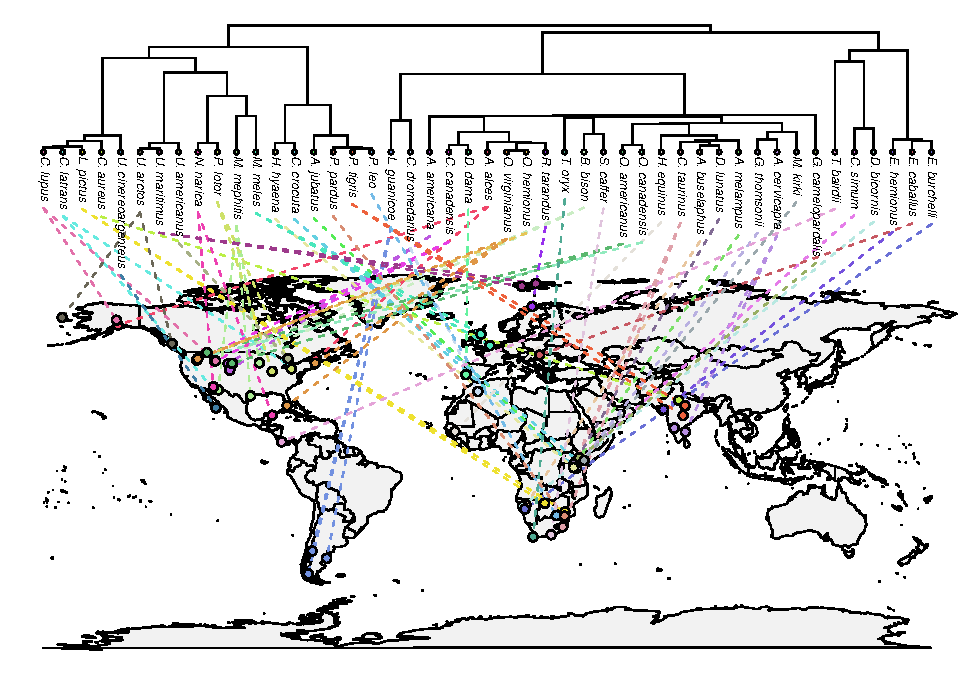
\includegraphics[width=1\linewidth]{old.Revell.phytools-v2_peerj_files/figure-latex/mammal-geog-1} %%%
\DIFdelendFL \DIFaddbeginFL 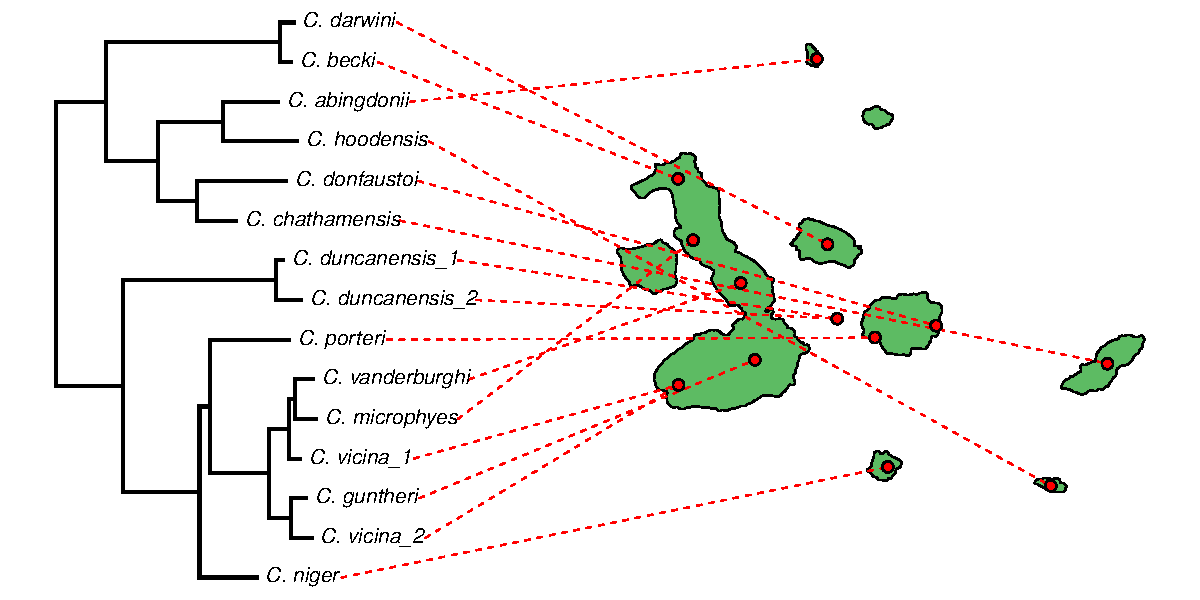
\includegraphics[width=1\linewidth]{Revell.phytools-v2_peerj_files/figure-latex/tortoise-geog-1} \DIFaddendFL \caption{A phylogenetic tree of \DIFdelbeginFL \DIFdelFL{mammals }\DIFdelendFL \DIFaddbeginFL \DIFaddFL{Galapagos tortoises }\DIFaddendFL projected onto a geographic map. \DIFdelbeginFL \DIFdelFL{Mammal phylogeny is from Garland }\DIFdelendFL \DIFaddbeginFL \DIFaddFL{Phylogenetic data and geographic locality information are based on Poulakakis }\DIFaddendFL et al. (\DIFdelbeginFL \DIFdelFL{1992}\DIFdelendFL \DIFaddbeginFL \DIFaddFL{2020}\DIFaddendFL )\DIFdelbeginFL \DIFdelFL{, and the geographic coordinates were selected from citizen science records}\DIFdelendFL . See main text for more details.}\DIFdelbeginFL %DIFDELCMD < \label{fig:mammal-geog}
%DIFDELCMD < %%%
\DIFdelendFL \DIFaddbeginFL \label{fig:tortoise-geog}
\DIFaddendFL \end{figure}

\DIFdelbegin \DIFdel{In this case, the lineages of our phylogeny in Figure
@ref(fig:mammal-geog) have a near-global distribution. For phylogenetic
trees whose terminal taxa have a narrower geographic range, including
phylogeographic studies, }\DIFdelend \DIFaddbegin \DIFadd{Although the base map from }\emph{\DIFadd{mapdata}} \DIFadd{is sufficiently high
resolution for our purposes here, higher resolution maps are available
for some regions, and }\DIFaddend it's \DIFdelbegin \DIFdel{possible to restrict the plotted maps to
countries or regions, or even to supply }\DIFdelend \DIFaddbegin \DIFadd{even possible to import and use }\DIFaddend a custom map
\DIFaddbegin \DIFadd{-- should we be so inclined }\DIFaddend (e.g., Quach et al. 2019)\DIFdelbegin \DIFdel{!
}\DIFdelend \DIFaddbegin \DIFadd{.
}\DIFaddend 

\hypertarget{projecting-trees-into-phenotypic-space}{%
\subsection{Projecting trees into phenotypic
space}\label{projecting-trees-into-phenotypic-space}}

Along with projecting a phylogenetic tree onto a geographic map (as we
just saw), and projecting traits onto the edges and nodes of a plotted
tree, the \emph{phytools} package also contains multiple methods to
project a tree into a space defined by our traits. Undoubtedly, the most
popular of these are \texttt{phylomorphospace}, which projects a tree
into a bivariate quantitative trait space (Sidlauskas 2008; e.g.,
Friedman et al. 2016; Martins et al. 2021), and \texttt{phenogram},
which projects a tree into a space defined by time since the root on the
horizontal and phenotype on the vertical (typically called a
``traitgram,'' see Evans et al. 2009; e.g., Martinez et al. 2020; Chazot
et al. 2021). We saw how \texttt{phenogram} works in Figure
@ref(fig:primate-edgewidth)b of any earlier section of this article.
Here, I'll focus on the \emph{phytools} method
\texttt{phylomorphospace}.

For this example I'll \DIFdelbegin \DIFdel{use }\DIFdelend \DIFaddbegin \DIFadd{be using }\DIFaddend a time-calibrated phylogeny of 11
vertebrate species from the \emph{TimeTree} website (Hedges et al.
2006), and a phenotypic trait dataset of body mass (in kg) and mean
litter size. (The latter dataset was generated from \emph{Wikipedia} and
other sources: i.e., ``Googling it.'')

\begin{Shaded}
\begin{Highlighting}[]
\FunctionTok{data}\NormalTok{(vertebrate.tree)}
\FunctionTok{data}\NormalTok{(vertebrate.data)}
\FunctionTok{head}\NormalTok{(vertebrate.data)}
\end{Highlighting}
\end{Shaded}

\begin{verbatim}
##                           Mass Length Litter_size
## Carcharodon_carcharias 2268.00  6.100        10.0
## Carassius_auratus         0.91  0.380       200.0
## Latimeria_chalumnae      80.00  2.000        15.0
## Iguana_iguana             8.00  2.000        50.5
## Turdus_migratorius        0.28  0.094         4.0
## Homo_sapiens             80.00  1.700         1.1
\end{verbatim}

\DIFdelbegin \DIFdel{(}\DIFdelend We should see that our data frame actually has three columns -- but
henceforward I'll just use the first and the third of these.
\DIFdelbegin \DIFdel{)
}\DIFdelend 

Normally, we could pass our data frame or matrix and phylogeny directly
to the \texttt{phylomorphospace} function and obtain a plot.
\texttt{phylomorphospace} would then undertake to project the tree,
using Maximum Likelihood reconstructed ancestral values for both traits
as the positions for internal nodes. \DIFaddbegin \DIFadd{In this case, however, }\DIFaddend I'd prefer
\DIFdelbegin \DIFdel{, however, }\DIFdelend to first reconstruct ancestral states on a log scale, back-transform my
estimated values to the original space, and then use these
back-transformed reconstruction as my node positions. Fortunately,
\texttt{phylomorphospace} allows that! \DIFaddbegin \DIFadd{(In addition to the reasoning I
provided in an earlier section, the logic of reconstructing ancestral
states on a log scale is because quantitative traits in general, and
morphometric data in particular, often satisfy the Brownian motion
assumption better on a logarithmic than linear scale. The reasoning of
back-transforming before plotting or reporting our results is simply
because most human brains, mine included, are more adept at interpreting
values on an additive rather than multiplicative scale!)
}\DIFaddend 

For the first step, I'll use the \emph{phytools} ancestral state
estimation function \texttt{fastAnc}. \texttt{fastAnc} computes Maximum
Likelihood ancestral states for one input character vector at a time, so
we just need to iterate across the two columns (of interest) in our data
frame using an \texttt{apply} call as follows.

\begin{Shaded}
\begin{Highlighting}[]
\NormalTok{vertebrate.ace}\OtherTok{\textless{}{-}}\FunctionTok{exp}\NormalTok{(}\FunctionTok{apply}\NormalTok{(}\FunctionTok{log}\DIFdelbegin \DIFdel{\NormalTok{(}
\NormalTok{  vertebrate.data[,}}\DIFdelend \DIFaddbegin \DIFadd{\NormalTok{(vertebrate.data[,}}\DIFaddend \FunctionTok{c}\NormalTok{(}\DecValTok{1}\NormalTok{,}\DecValTok{3}\NormalTok{)]),}
  \DecValTok{2}\DIFdelbegin \DIFdel{\NormalTok{,}
\NormalTok{  fastAnc,}}\DIFdelend \DIFaddbegin \DIFadd{\NormalTok{,fastAnc,}}\DIFaddend \AttributeTok{tree=}\NormalTok{vertebrate.tree))}
\NormalTok{vertebrate.ace}
\end{Highlighting}
\end{Shaded}

\begin{verbatim}
##          Mass Litter_size
## 12  25.571594   15.552422
## 13  17.834793   16.114126
## 14  16.827622   14.481309
## 15   8.801275    8.791375
## 16  20.362215    1.653955
## 17  17.335294    1.442396
## 18  24.604666    1.610416
## 19 152.078728    1.737334
## 20 301.219076    1.582780
## 21   6.329908    9.613237
\end{verbatim}

This gives us a set of reconstructed values on our original (linear)
scale, but in which the reconstruction was performed on a \emph{log}
scale, and then back-transformed. Finally, let's create our
phylomorphospace plot.

\begin{Shaded}
\begin{Highlighting}[]
\FunctionTok{par}\NormalTok{(}\AttributeTok{mar=}\FunctionTok{c}\NormalTok{(}\FloatTok{5.1}\NormalTok{,}\FloatTok{4.1}\NormalTok{,}\FloatTok{0.6}\NormalTok{,}\FloatTok{2.1}\NormalTok{))}
\FunctionTok{phylomorphospace}\NormalTok{(vertebrate.tree,}
\NormalTok{  vertebrate.data[,}\FunctionTok{c}\NormalTok{(}\DecValTok{1}\NormalTok{,}\DecValTok{3}\NormalTok{)],}\AttributeTok{A=}\NormalTok{vertebrate.ace,}\AttributeTok{log=}\StringTok{"xy"}\NormalTok{,}
  \AttributeTok{xlim=}\FunctionTok{c}\NormalTok{(}\FloatTok{1e{-}4}\NormalTok{,}\FloatTok{1e6}\NormalTok{),}\AttributeTok{ylim=}\FunctionTok{c}\NormalTok{(}\FloatTok{0.5}\NormalTok{,}\DecValTok{200}\NormalTok{),}\AttributeTok{bty=}\StringTok{"n"}\NormalTok{,}\AttributeTok{label=}\StringTok{"off"}\NormalTok{,}
  \AttributeTok{axes=}\ConstantTok{FALSE}\NormalTok{,}\AttributeTok{xlab=}\StringTok{"Mass (kg)"}\NormalTok{,}\AttributeTok{ylab=}\StringTok{"Litter size"}\NormalTok{,}
  \AttributeTok{node.size=}\FunctionTok{c}\NormalTok{(}\DecValTok{0}\NormalTok{,}\DecValTok{0}\NormalTok{))}
\FunctionTok{axis}\NormalTok{(}\DecValTok{1}\NormalTok{,}\AttributeTok{at=}\DecValTok{10}\SpecialCharTok{\^{}}\FunctionTok{seq}\NormalTok{(}\SpecialCharTok{{-}}\DecValTok{3}\NormalTok{,}\DecValTok{5}\NormalTok{,}\AttributeTok{by=}\DecValTok{2}\NormalTok{),}
  \AttributeTok{labels=}\FunctionTok{prettyNum}\NormalTok{(}\DecValTok{10}\SpecialCharTok{\^{}}\FunctionTok{seq}\NormalTok{(}\SpecialCharTok{{-}}\DecValTok{3}\NormalTok{,}\DecValTok{5}\NormalTok{,}\AttributeTok{by=}\DecValTok{2}\NormalTok{),}\AttributeTok{big.mark=}\StringTok{","}\NormalTok{),}
  \AttributeTok{las=}\DecValTok{1}\NormalTok{,}\AttributeTok{cex.axis=}\FloatTok{0.6}\NormalTok{)}
\FunctionTok{axis}\NormalTok{(}\DecValTok{2}\NormalTok{,}\AttributeTok{at=}\DecValTok{10}\SpecialCharTok{\^{}}\FunctionTok{seq}\NormalTok{(}\DecValTok{0}\NormalTok{,}\DecValTok{2}\NormalTok{,}\AttributeTok{by=}\DecValTok{1}\NormalTok{),}
  \AttributeTok{labels=}\FunctionTok{prettyNum}\NormalTok{(}\DecValTok{10}\SpecialCharTok{\^{}}\FunctionTok{seq}\NormalTok{(}\DecValTok{0}\NormalTok{,}\DecValTok{2}\NormalTok{,}\AttributeTok{by=}\DecValTok{1}\NormalTok{),}\AttributeTok{big.mark=}\StringTok{","}\NormalTok{),}
  \AttributeTok{las=}\DecValTok{1}\NormalTok{,}\AttributeTok{cex.axis=}\FloatTok{0.7}\NormalTok{)}
\NormalTok{cols}\OtherTok{\textless{}{-}}\FunctionTok{setNames}\NormalTok{(RColorBrewer}\SpecialCharTok{::}\FunctionTok{brewer.pal}\NormalTok{(}
  \FunctionTok{nrow}\NormalTok{(vertebrate.data),}\StringTok{"Paired"}\NormalTok{),}
  \FunctionTok{rownames}\NormalTok{(vertebrate.data))}
\FunctionTok{points}\NormalTok{(vertebrate.data[,}\FunctionTok{c}\NormalTok{(}\DecValTok{1}\NormalTok{,}\DecValTok{3}\NormalTok{)],}\AttributeTok{pch=}\DecValTok{21}\NormalTok{,}\AttributeTok{bg=}\NormalTok{cols,}\AttributeTok{cex=}\FloatTok{1.2}\NormalTok{)}
\NormalTok{ind}\OtherTok{\textless{}{-}}\FunctionTok{order}\NormalTok{(}\FunctionTok{rownames}\NormalTok{(vertebrate.data))}
\FunctionTok{legend}\NormalTok{(}\StringTok{"topleft"}\NormalTok{,}\FunctionTok{gsub}\NormalTok{(}\StringTok{"\_"}\NormalTok{,}\StringTok{" "}\NormalTok{,}
  \FunctionTok{rownames}\NormalTok{(vertebrate.data))[ind],}\AttributeTok{pch=}\DecValTok{21}\NormalTok{,}\AttributeTok{pt.cex=}\FloatTok{1.2}\NormalTok{,}
  \AttributeTok{pt.bg=}\NormalTok{cols[ind],}\AttributeTok{cex=}\FloatTok{0.6}\NormalTok{,}\AttributeTok{bty=}\StringTok{"n"}\NormalTok{,}\AttributeTok{text.font=}\DecValTok{3}\NormalTok{)}
\end{Highlighting}
\end{Shaded}

\begin{figure}
\DIFdelbeginFL %DIFDELCMD < \includegraphics[width=1\linewidth]{old.Revell.phytools-v2_peerj_files/figure-latex/vert-phylomorphospace-1} %%%
\DIFdelendFL \DIFaddbeginFL \includegraphics[width=1\linewidth]{Revell.phytools-v2_peerj_files/figure-latex/vert-phylomorphospace-1} \DIFaddendFL \caption{Phylomorphospace of body mass and litter size for a selection of vertebrate species. \DIFaddbeginFL \DIFaddFL{The uderlying phylogenetic tree was obtained from Hedges et al. (2006). }\DIFaddendFL See main text for additional details.}\label{fig:vert-phylomorphospace}
\end{figure}

\DIFdelbegin \DIFdel{In this code}\DIFdelend \DIFaddbegin \DIFadd{Here}\DIFaddend , I chose to graph the projection without taxon labels, then add
different colored points and a legend to put the label information back
on the plot (sorting my labels alphabetically as I did this). As readers
can probably imagine, taxon labels on a phylomorphospace plot can easily
become very messy -- particularly for larger trees!

\hypertarget{plotting-phenotypic-data-at-the-tips-of-the-tree}{%
\subsection{Plotting phenotypic data at the tips of the
tree}\label{plotting-phenotypic-data-at-the-tips-of-the-tree}}

In addition to projecting phylogenies into trait spaces, and plotting
observed or reconstructed trait values on the tree, \emph{phytools}
\DIFaddbegin \DIFadd{possesses a number of different plotting methods that }\DIFaddend can also help us
undertake the (at least, conceptually) simple task of visualizing
comparative trait data for species at the tips of the tree.

This might be done in various ways. For instance, we could graph the
values of a quantitative trait adjacent to the tip labels using a bar or
box, or we might plot the presence or absence of different lineages from
a habitat type next to the tips of the tree \DIFaddbegin \DIFadd{(Revell 2014b)}\DIFaddend . Numerous
such approaches have been developed and implemented in the
\emph{phytools} package, and many of these are shown in my recent book
(Revell and Harmon 2022).

Here, I'll illustrate just one such method in which a color gradient is
used to visualize trait values for a set of quantitative characters at
the tips of the tree \DIFaddbegin \DIFadd{(Revell 2014b)}\DIFaddend . The \emph{phytools} implementation
of this plotting method is called \texttt{phylo.heatmap}, and it's been
used in numerous published articles (e.g., Goelen et al. 2020; Hultgren
et al. 2021; Molina-Mora et al. 2021; Huang et al. 2022\DIFaddbegin \DIFadd{; Morales-Poole
et al. 2022}\DIFaddend ). For this example, we'll use a phylogenetic tree and
\DIFaddbegin \DIFadd{log-transformed }\DIFaddend morphological trait dataset for \emph{Anolis} lizards
from (Mahler et al. 2010). To load these data, readers should run the
following.

\begin{Shaded}
\begin{Highlighting}[]
\FunctionTok{data}\NormalTok{(anoletree)}
\FunctionTok{data}\NormalTok{(anole.data)}
\FunctionTok{head}\NormalTok{(anole.data)}
\end{Highlighting}
\end{Shaded}

\begin{verbatim}
##                 SVL      HL     HLL     FLL     LAM      TL
## ahli        4.03913 2.88266 3.96202 3.34498 2.86620 4.50400
## allogus     4.04014 2.86103 3.94018 3.33829 2.80827 4.52189
## rubribarbus 4.07847 2.89425 3.96135 3.35641 2.86751 4.56108
## imias       4.09969 2.85293 3.98565 3.41402 2.94375 4.65242
## sagrei      4.06716 2.83515 3.85786 3.24267 2.91872 4.77603
## bremeri     4.11337 2.86044 3.90039 3.30585 2.97009 4.72996
\end{verbatim}

Our trait data object, \texttt{anole.data}, is a data frame with six
trait columns for various phylogenetic traits.

We could visualize our data directly; however, the effect of overall
size (data column \texttt{"SVL"}) would tend to obscure any interesting
patterns of residual variation and covariation in body shape among the
species in our tree. As such, primarily in an effort to control for
overall size, I'll first run a phylogenetic principal components
analysis (Revell 2009) using the \emph{phytools} function
\texttt{phyl.pca}. A phylogenetic principal components analysis
(mentioned earlier with respect to the Broeckhoven et al. 2016 dataset)
is similar to a regular PCA except that we account for non-independence
of the information for different species in our data rotation (Revell
2009).

\begin{Shaded}
\begin{Highlighting}[]
\NormalTok{anole.ppca}\OtherTok{\textless{}{-}}\FunctionTok{phyl.pca}\NormalTok{(anoletree,anole.data,}\AttributeTok{mode=}\StringTok{"corr"}\NormalTok{)}
\NormalTok{anole.ppca}
\end{Highlighting}
\end{Shaded}

\begin{verbatim}
## Phylogenetic pca
## Standard deviations:
##       PC1       PC2       PC3       PC4       PC5       PC6 
## 2.2896942 0.6674345 0.4381067 0.2997973 0.1395612 0.1026573 
## Loads:
##            PC1         PC2         PC3         PC4           PC5
## SVL -0.9782776 -0.01988115  0.14487425 -0.11332244  0.0781070110
## HL  -0.9736568 -0.03879982  0.13442473 -0.15596460 -0.0852979941
## HLL -0.9711545  0.14491400  0.02151524  0.17058611 -0.0588208480
## FLL -0.9759133 -0.02087140  0.14486273  0.14149988  0.0475205990
## LAM -0.8299594 -0.50437051 -0.23796010  0.01194704  0.0004983465
## TL  -0.8679195  0.40956428 -0.27350654 -0.05871034  0.0195584629
##              PC6
## SVL -0.051442939
## HL   0.028570939
## HLL -0.053257988
## FLL  0.062386141
## LAM -0.003133966
## TL   0.018373275
\end{verbatim}

Our PC loadings show us the the first principal component dimension is
strongly negatively correlated with all of the traits in our analysis.
We could consider this the ``size'' axis. Principal component 2 is most
strongly (negatively) correlated with the character \texttt{"LAM"},
number of adhesive toepad scales called lamellae; and most positively
correlated with \texttt{"TL"}, tail length.

Let's compute the principal component scores for all of our species.

\begin{Shaded}
\begin{Highlighting}[]
\NormalTok{anole.pc\_scores}\OtherTok{\textless{}{-}}\FunctionTok{scores}\NormalTok{(anole.ppca)}
\FunctionTok{head}\NormalTok{(anole.pc\_scores)}
\end{Highlighting}
\end{Shaded}

\begin{verbatim}
##                    PC1       PC2         PC3       PC4         PC5
## ahli        -0.1747576 0.8697064  1.52379491 1.6029659 -0.23955421
## allogus      0.1646585 1.4017806  1.74506491 1.5358005 -0.08089546
## rubribarbus -0.4925001 1.0413268  1.45866163 1.4180850 -0.05716104
## imias       -1.1608049 0.7514380  0.75822327 1.7127381  0.35013533
## sagrei      -0.3486332 1.2632997 -0.05102313 0.7317455  0.37217463
## bremeri     -0.9714818 0.6943196  0.11689334 0.9290039  0.43486041
##                    PC6
## ahli        -0.1626049
## allogus     -0.1245855
## rubribarbus -0.1797060
## imias       -0.1340347
## sagrei      -0.1484157
## bremeri     -0.2304513
\end{verbatim}

Since the sign of each principal component is arbitrary (principal
components are vectors), we'll now ``flip'' the sign of PC 1 -- so that
it switches from negative size to simply ``size.''

\begin{Shaded}
\begin{Highlighting}[]
\NormalTok{anole.pc\_scores[,}\DecValTok{1}\NormalTok{]}\OtherTok{\textless{}{-}}\SpecialCharTok{{-}}\NormalTok{anole.pc\_scores[,}\DecValTok{1}\NormalTok{]}
\FunctionTok{head}\NormalTok{(anole.pc\_scores)}
\end{Highlighting}
\end{Shaded}

\begin{verbatim}
##                    PC1       PC2         PC3       PC4         PC5
## ahli         0.1747576 0.8697064  1.52379491 1.6029659 -0.23955421
## allogus     -0.1646585 1.4017806  1.74506491 1.5358005 -0.08089546
## rubribarbus  0.4925001 1.0413268  1.45866163 1.4180850 -0.05716104
## imias        1.1608049 0.7514380  0.75822327 1.7127381  0.35013533
## sagrei       0.3486332 1.2632997 -0.05102313 0.7317455  0.37217463
## bremeri      0.9714818 0.6943196  0.11689334 0.9290039  0.43486041
##                    PC6
## ahli        -0.1626049
## allogus     -0.1245855
## rubribarbus -0.1797060
## imias       -0.1340347
## sagrei      -0.1484157
## bremeri     -0.2304513
\end{verbatim}

Finally, let's graph our results using the \texttt{phylo.heatmap}
function. Seeing as the variance in our different principal component
dimensions are quite different from PC to PC, we'll standardize them to
have a constant variance using \texttt{standardize=TRUE}. As we've done
in other exercises of this article, we can update the default color
palette of the plot using the argument \texttt{colors}. Here, I'll use
the colorblind-friendly \DIFdelbegin \texttt{\DIFdel{viridis}} %DIFAUXCMD
\DIFdelend \DIFaddbegin \DIFadd{viridis }\DIFaddend color palette from the
\emph{viridisLite} package (Garnier et al. 2022) \DIFaddbegin \DIFadd{that we learned about
earlier}\DIFaddend .

\begin{Shaded}
\begin{Highlighting}[]
\FunctionTok{phylo.heatmap}\NormalTok{(anoletree,anole.pc\_scores,}
  \AttributeTok{standardize=}\ConstantTok{TRUE}\NormalTok{,}\AttributeTok{fsize=}\FunctionTok{c}\NormalTok{(}\FloatTok{0.4}\NormalTok{,}\FloatTok{0.7}\NormalTok{,}\FloatTok{0.7}\NormalTok{),}\AttributeTok{pts=}\ConstantTok{FALSE}\NormalTok{,}
  \AttributeTok{split=}\FunctionTok{c}\NormalTok{(}\FloatTok{0.6}\NormalTok{,}\FloatTok{0.4}\NormalTok{),}\AttributeTok{colors=}\NormalTok{viridisLite}\SpecialCharTok{::}\FunctionTok{viridis}\NormalTok{(}\AttributeTok{n=}\DecValTok{40}\NormalTok{,}
  \AttributeTok{direction=}\SpecialCharTok{{-}}\DecValTok{1}\NormalTok{),}\AttributeTok{mar=}\FunctionTok{rep}\NormalTok{(}\FloatTok{0.1}\NormalTok{,}\DecValTok{4}\NormalTok{))}
\end{Highlighting}
\end{Shaded}

\begin{figure}
\DIFdelbeginFL %DIFDELCMD < \includegraphics[width=1\linewidth]{old.Revell.phytools-v2_peerj_files/figure-latex/anole-heatmap-1} %%%
\DIFdelendFL \DIFaddbeginFL \includegraphics[width=1\linewidth]{Revell.phytools-v2_peerj_files/figure-latex/anole-heatmap-1} \DIFaddendFL \caption{Phylogenetic heatmap showing principal components from a phylogenetic PCA of six morphological traits of \textit{Anolis} lizards. Tree and data \DIFaddbeginFL \DIFaddFL{are }\DIFaddendFL from Mahler et al. (2010). See main text for additional details.}\label{fig:anole-heatmap}
\end{figure}

In Figure @ref(fig:anole-heatmap) we can already begin to discern some
of the interesting ecomorphological phenotypic patterns of \emph{Anolis}
lizards (Losos 2009). For instance, the largest species (known as
``crown-giants\DIFdelbegin \DIFdel{''}\DIFdelend \DIFaddbegin \DIFadd{,'' Losos 2009}\DIFaddend ), that is, those species with the highest
values of PC 1, tend to have moderate or low values for PC 2: meaning
they have larger lamellae and shorter tails, controlling for their body
size. By contrast some of the smallest species (on PC 1) have among the
highest values for PC 2 (tail length). These are the ``grass-bush''
anoles that perch on grass and bushes near the grown, and use their long
tails to control body pitch while jumping. \DIFaddbegin \DIFadd{We can likewise see that this
combination of phenotypic traits (large body size and large lamellae;
small body size and long tail) has evolved }\emph{\DIFadd{independently}} \DIFadd{in
different parts of the phylogenetic tree. Just by visualizing our data
and learning this, we're already doing phylogenetic comparative methods.
}\DIFaddend Neat!

\hypertarget{relationship-of-phytools-to-other-packages}{%
\section{\texorpdfstring{Relationship of \emph{phytools} to other
packages}{Relationship of phytools to other packages}}\label{relationship-of-phytools-to-other-packages}}

The \emph{phytools} package has grown to become (along with \emph{ape},
\emph{phangorn}, and \emph{geiger}) among the most important core
packages for phylogenetic analysis in the R environment. As of the time
of writing, the original publication describing \emph{phytools} (Revell,
2012) had been cited more than \DIFdelbegin \DIFdel{6,700 }\DIFdelend \DIFaddbegin \DIFadd{7,300 }\DIFaddend times on \emph{Google Scholar} and
continues to be cited over 1,000 times per year.

In many respect, however, \emph{phytools} owes its existence to a number
of other packages making up the R phylogenetics ecosytem and from which
it imports crtical functionality. In particular, \emph{phytools} depends
on the object classes and methods of the core R phylogenetics package,
\emph{ape} (Paradis et al. 2004; Popescu et al. 2012; Paradis and
Schliep 2019). In addition, \emph{phytools} relies on a number of
different methods from the multifunctional phylogenetic inference
package, \emph{phangorn} (Schliep 2011). Finally, \emph{phytools} is
designed to interact with a variety of other function R phylogenetics
libraries, especially the \emph{geiger} package (Harmon et al. 2008;
Pennell et al. 2014), which \emph{phytools} ``suggests'' but does not
import.

Outside phylogenetics as such, \emph{phytools} also presently depends on
or imports from a number of other R packages including
\emph{clusterGeneration} (Qiu and Joe. 2020), \emph{coda} (Plummer et
al. 2006), \emph{combinat} (Chasalow 2012), \emph{doParallel}
(Corporation and Weston 2022), \emph{expm} (Maechler et al. 2023),
\emph{foreach} (Microsoft and Weston 2022), \emph{maps} (Becker et al.
\DIFdelbegin \DIFdel{2022}\DIFdelend \DIFaddbegin \DIFadd{2022a}\DIFaddend ), \emph{MASS} (Venables and Ripley 2002), \emph{mnormt} (Azzalini
and Genz 2022), \emph{nlme} (Pinheiro and Bates 2000; Pinheiro et al.
2022), \emph{numDeriv} (Gilbert and Varadhan 2019), \emph{optimParallel}
(Gerber and Furrer 2019), \emph{plotrix} (J 2006), and
\emph{scatterplot3d} (Ligges and Mächler 2003), although dependency
relationships are dynamic as packages evolve and may change.

\hypertarget{conclusions}{%
\section{Conclusions}\label{conclusions}}

More than a decade has passed since the original and only article
describing \emph{phytools} was published (Revell 2012). Since that time,
the \emph{phytools} package has both evolved into one of the core
function libraries of the R phylogenetics ecosystem, and expanded
manyfold in size and scope. As such, I decided the literature reference
for \emph{phytools} was sorely in need of updating. In creating one,
however, I was determined to make something that could serve as more
than a placeholder to capture citations of the \emph{phytools} package.
I hope that what I've provided here will help guide \DIFaddbegin \DIFadd{some }\DIFaddend new
\emph{phytools} users towards interesting analytical tools, as well as
perhaps inspire experienced \emph{phytools} and R phylogenetics
researchers to generate new types of questions and data that will in
turn help motivate continued development of the \emph{phytools} package
into the future.

\hypertarget{software-and-data-availability}{%
\section{Software and data
availability}\label{software-and-data-availability}}

The \emph{phytools} \DIFaddbegin \DIFadd{R package }\DIFaddend is free and open source, and can be
downloaded from its CRAN
(\url{https://CRAN.R-project.org/package=phytools}) or GitHub
(\url{https://github.com/liamrevell/phytools}) pages. \DIFaddbegin \DIFadd{More information
about the }\emph{\DIFadd{phytools}} \DIFadd{package can be obtained from the software
documentation pages, my }\emph{\DIFadd{phytools}} \DIFadd{blog
(}\url{http://blog.phytools.org}\DIFadd{), or via my recent book with Luke Harmon
(Revell and Harmon 2022).
}\DIFaddend 

This article was written in Rmarkdown (Xie et al. 2018, 2020; Allaire et
al. 2023), and developed with the help of both \emph{bookdown} (Xie
2016, 2023) and the posit Rstudio IDE (RStudio Team 2020). \DIFdelbegin %DIFDELCMD < 

%DIFDELCMD < %%%
\DIFdelend Markdown code
and data files necessary to exactly reproduce the analyses of this
article are available at
\url{https://github.com/liamrevell/Revell.phytools-v2/} \DIFaddbegin \DIFadd{(and folders
therein)}\DIFaddend .

\hypertarget{references}{%
\section*{References}\label{references}}
\addcontentsline{toc}{section}{References}

\hypertarget{refs}{}
\begin{CSLReferences}{1}{0}
\leavevmode\vadjust pre{\hypertarget{ref-Allaire2023}{}}%
Allaire, J., Y. Xie, J. McPherson, J. Luraschi, K. Ushey, A. Atkins, H.
Wickham, J. Cheng, W. Chang, and R. Iannone. 2023.
\href{https://github.com/rstudio/rmarkdown}{Rmarkdown: Dynamic documents
for {R}}.

\leavevmode\vadjust pre{\hypertarget{ref-Amarasinghe2021}{}}%
Amarasinghe, P., S. Joshi, N. Page, L. S. Wijedasa, M. Merello, H.
Kathriarachchi, R. D. Stone, W. Judd, U. Kodandaramaiah, and N.
Cellinese. 2021. Evolution and biogeography of memecylon. Am. J. Bot.
108:628--646. Wiley.

\leavevmode\vadjust pre{\DIFdelbegin %DIFDELCMD < \hypertarget{ref-Ammar2019}{}}%%%
%DIF < 
\DIFdel{Ammar, R. 2019.
}\href{https://CRAN.R-project.org/package=randomcoloR}{\DIFdel{randomcoloR:
Generate attractive random colors}}%DIFAUXCMD
\DIFdel{.
}%DIFDELCMD < 

%DIFDELCMD < \leavevmode\vadjust %%%
\DIFdel{pre}%DIFDELCMD < {%%%
\DIFdelend \hypertarget{ref-Atkinson2020}{}}%
Atkinson, C. L., B. C. Ee, and J. M. Pfeiffer. 2020.
\href{https://doi.org/10.1002/ecy.3100}{Evolutionary history drives
aspects of stoichiometric niche variation and functional effects within
a guild}. Ecology 101:e03100. Wiley.

\leavevmode\vadjust pre{\hypertarget{ref-Azzalini2022}{}}%
Azzalini, A., and A. Genz. 2022.
\href{http://azzalini.stat.unipd.it/SW/Pkg-mnormt/}{The {R} package
\texttt{mnormt}: The multivariate normal and \(t\) distributions
(version 2.1.1)}.

\leavevmode\vadjust pre{\hypertarget{ref-Baele2018-wc}{}}%
Baele, G., S. Dellicour, M. A. Suchard, P. Lemey, and B. Vrancken. 2018.
Recent advances in computational phylodynamics. Curr. Opin. Virol.
31:24--32. Elsevier BV.

\leavevmode\vadjust pre{\DIFaddbegin \hypertarget{ref-Bartoszek2012}{}}%DIF > 
\DIFadd{Bartoszek, K., J. Pienaar, P. Mostad, S. Andersson, and T. F. Hansen.
2012. A phylogenetic comparative method for studying multivariate
adaptation. Journal of Theoretical Biology 314:204--215.
}

\leavevmode\vadjust \DIFadd{pre}{\hypertarget{ref-Bastide2018}{}}%DIF > 
\DIFadd{Bastide, P., C. Ané, S. Robin, and M. Mariadassou. 2018.
}\href{https://doi.org/10.1093/sysbio/syy005}{\DIFadd{Inference of adaptive
shifts for multivariate correlated traits}}\DIFadd{. Systematic Biology
67:662--680. Oxford University Press (}{\DIFadd{OUP}}\DIFadd{).
}

\leavevmode\vadjust \DIFadd{pre}{\DIFaddend \hypertarget{ref-Beale2019-bx}{}}%
Beale, M. A., M. Marks, S. K. Sahi, L. C. Tantalo, A. V. Nori, P.
French, S. A. Lukehart, C. M. Marra, and N. R. Thomson. 2019. Genomic
epidemiology of syphilis reveals independent emergence of macrolide
resistance across multiple circulating lineages. Nat. Commun. 10:3255.
Springer Science; Business Media LLC.

\leavevmode\vadjust pre{\hypertarget{ref-Beaulieu2016-hisse}{}}%
Beaulieu, J. M., and B. C. O'Meara. 2016.
\href{https://academic.oup.com/sysbio/article/65/4/583/1753616}{Detecting
hidden diversification shifts in models of trait-dependent speciation
and extinction.} Systematic Biology 65:583--601.

\leavevmode\vadjust pre{\hypertarget{ref-Beaulieu2013-zo}{}}%
Beaulieu, J. M., B. C. O'Meara, and M. J. Donoghue. 2013. Identifying
hidden rate changes in the evolution of a binary morphological
character: The evolution of plant habit in campanulid angiosperms. Syst.
Biol. 62:725--737.

\leavevmode\vadjust pre{\DIFaddbegin \hypertarget{ref-Beaulieu2022-corhmm}{}}%DIF > 
\DIFadd{Beaulieu, J., B. O'Meara, J. Oliver, and J. Boyko. 2022.
}\href{https://CRAN.R-project.org/package=corHMM}{{\DIFadd{corHMM}}\DIFadd{: }{\DIFadd{H}}\DIFadd{idden
}{\DIFadd{M}}\DIFadd{arkov models of character evolution}}\DIFadd{.
}

\leavevmode\vadjust \DIFadd{pre}{\DIFaddend \hypertarget{ref-Becker2022}{}}%
Becker, R. A., A. R. Wilks, R. Brownrigg, T. P. Minka, and A. Deckmyn.
\DIFdelbegin \DIFdel{2022. }\DIFdelend \DIFaddbegin \DIFadd{2022a. }\DIFaddend \href{https://CRAN.R-project.org/package=maps}{Maps: Draw
geographical maps}.

\leavevmode\vadjust pre{\DIFaddbegin \hypertarget{ref-Becker2022-mapdata}{}}%DIF > 
\DIFadd{Becker, R. A., A. R. Wilks, and R. Brownrigg. 2022b.
}\href{https://CRAN.R-project.org/package=mapdata}{\DIFadd{Mapdata: Extra map
databases}}\DIFadd{.
}

\leavevmode\vadjust \DIFadd{pre}{\DIFaddend \hypertarget{ref-Bentz2018-xa}{}}%
Bentz, C., D. Dediu, A. Verkerk, and G. Jäger. 2018. The evolution of
language families is shaped by the environment beyond neutral drift.
Nat. Hum. Behav. 2:816--821. Springer Science; Business Media LLC.

\leavevmode\vadjust pre{\hypertarget{ref-Blinkhorn2021-gk}{}}%
Blinkhorn, J., and M. Grove. 2021. Explanations of variability in
{M}iddle {S}tone {A}ge stone tool assemblage composition and raw
material use in {E}astern {A}frica. Archaeol. Anthropol. Sci. 13:14.
Springer Science; Business Media LLC.

\leavevmode\vadjust pre{\hypertarget{ref-Blomberg2003-as}{}}%
Blomberg, S. P., T. Garland Jr, and A. R. Ives. 2003. Testing for
phylogenetic signal in comparative data: Behavioral traits are more
labile. Evolution 57:717--745.

\leavevmode\vadjust pre{\DIFaddbegin \hypertarget{ref-Bollback2006}{}}%DIF > 
\DIFadd{Bollback, J. P. 2006.
}\href{https://doi.org/10.1186/1471-2105-7-88}{{\DIFadd{SIMMAP}}\DIFadd{: Stochastic
character mapping of discrete traits on phylogenies}}\DIFadd{. }{\DIFadd{BMC}}
\DIFadd{Bioinformatics 7:88. Springer Science; Business Media }{\DIFadd{LLC}}\DIFadd{.
}

\leavevmode\vadjust \DIFadd{pre}{\DIFaddend \hypertarget{ref-Broeckhoven2016}{}}%
Broeckhoven, C., G. Diedericks, C. Hui, B. G. Makhubo, and P. le Fras N.
Mouton. 2016. \href{https://doi.org/10.1111/evo.13062}{Enemy at the
gates: Rapid defensive trait diversification in an adaptive radiation of
lizards}. Evolution 70:2647--2656. Wiley.

\leavevmode\vadjust pre{\DIFaddbegin \hypertarget{ref-Burnham2003-mt}{}}%DIF > 
\DIFadd{Burnham, K. P., and D. R. Anderson. 2003. Model selection and multimodel
inference: A practical information theoretic approach. Springer Science
\& Business Media.
}

\leavevmode\vadjust \DIFadd{pre}{\DIFaddend \hypertarget{ref-Bushman2019-fs}{}}%
Bushman, F. D., K. McCormick, and S. Sherrill-Mix. 2019. Virus
structures constrain transmission modes. Nat. Microbiol. 4:1778--1780.
Springer Science; Business Media LLC.

\leavevmode\vadjust pre{\hypertarget{ref-Butler2004-av}{}}%
Butler, M. A., and A. A. King. 2004. Phylogenetic comparative analysis:
A modeling approach for adaptive evolution. Am. Nat. 164:683--695.

\leavevmode\vadjust pre{\DIFaddbegin \hypertarget{ref-Caetano2017}{}}%DIF > 
\DIFadd{Caetano, D. S., and L. J. Harmon. 2017.
}\href{https://doi.org/10.1111/2041-210x.12826}{\DIFadd{Ratematrix: An }{\DIFadd{R}}
\DIFadd{package for studying evolutionary integration among several traits on
phylogenetic trees}}\DIFadd{. Methods in Ecology and Evolution 8:1920--1927.
Wiley.
}

\leavevmode\vadjust \DIFadd{pre}{\DIFaddend \hypertarget{ref-Caraballo2022-rd}{}}%
Caraballo, D. A. 2022. Cross-species transmission of bat coronaviruses
in the americas: Contrasting patterns between alphacoronavirus and
betacoronavirus. Microbiol. Spectr. 10:e0141122. American Society for
Microbiology.

\leavevmode\vadjust pre{\hypertarget{ref-Chasalow2012}{}}%
Chasalow, S. 2012.
\href{https://CRAN.R-project.org/package=combinat}{Combinat:
Combinatorics utilities}.

\leavevmode\vadjust pre{\hypertarget{ref-Chazot2021-ey}{}}%
Chazot, N., P. Blandin, V. Debat, M. Elias, and F. L. Condamine. 2021.
Punctuational ecological changes rather than global factors drive
species diversification and the evolution of wing phenotypes in morpho
butterflies. J. Evol. Biol. 34:1592--1607. Wiley.

\leavevmode\vadjust pre{\DIFaddbegin \hypertarget{ref-Clavel2015}{}}%DIF > 
\DIFadd{Clavel, J., G. Escarguel, and G. Merceron. 2015. Mv}{\DIFadd{MORPH}}\DIFadd{: An }{\DIFadd{R}}
\DIFadd{package for fitting multivariate evolutionary models to morphometric
data. Methods in Ecology and Evolution 6:1311--1319.
}

\leavevmode\vadjust \DIFadd{pre}{\DIFaddend \hypertarget{ref-Collar2014-sw}{}}%
Collar, D. C., P. C. Wainwright, M. E. Alfaro, L. J. Revell, and R. S.
Mehta. 2014. Biting disrupts integration to spur skull evolution in
eels. Nature 5:5505.

\leavevmode\vadjust pre{\hypertarget{ref-Compton2023-nc}{}}%
Compton, Z., V. Harris, W. Mellon, S. Rupp, D. Mallo, S. E. Kapsetaki,
M. Wilmot, R. Kennington, K. Noble, C. Baciu, L. Ramirez, A. Peraza, B.
Martins, S. Sudhakar, S. Aksoy, G. Furukawa, O. Vincze, M. Giraudeau, E.
G. Duke, S. Spiro, E. Flach, H. Davidson, A. Zehnder, T. A. Graham, B.
Troan, T. M. Harrison, M. Tollis, J. D. Schiffman, A. Aktipis, L. M.
Abegglen, C. C. Maley, and A. M. Boddy. 2023. Cancer prevalence across
vertebrates. bioRxivorg.

\leavevmode\vadjust pre{\hypertarget{ref-Microsoft2022-a}{}}%
Corporation, M., and S. Weston. 2022.
\href{https://CRAN.R-project.org/package=doParallel}{doParallel: Foreach
parallel adaptor for the 'parallel' package}.

\leavevmode\vadjust pre{\hypertarget{ref-Csosz2016}{}}%
Csosz, S., and B. Fisher. 2016.
\href{https://doi.org/10.3897/zookeys.603.8271}{Taxonomic revision of
the malagasy nesomyrmex madecassus species-group using a quantitative
morphometric approach}. {ZooKeys} 603:105--130. Pensoft Publishers.

\leavevmode\vadjust pre{\DIFaddbegin \hypertarget{ref-Damian_Serrano_2021}{}}%DIF > 
\DIFadd{Damian-Serrano, A., S. H. D. Haddock, and C. W. Dunn. 2021.
}\href{https://doi.org/10.1073/pnas.2005063118}{\DIFadd{The evolution of
siphonophore tentilla for specialized prey capture in the open ocean}}\DIFadd{.
Proceedings of the National Academy of Sciences 118. Proceedings of the
National Academy of Sciences.
}

\leavevmode\vadjust \DIFadd{pre}{\DIFaddend \hypertarget{ref-Efron1983-al}{}}%
Efron, B., and G. Gong. 1983. A leisurely look at the bootstrap, the
jackknife, and cross-validation. Am. Stat. 37:36--48. Informa UK
Limited.

\leavevmode\vadjust pre{\hypertarget{ref-Endara2018}{}}%
Endara, M.-J., J. A. Nicholls, P. D. Coley, D. L. Forrister, G. C.
Younkin, K. G. Dexter, C. A. Kidner, R. T. Pennington, G. N. Stone, and
T. A. Kursar. 2018. Tracking of host defenses and phylogeny during the
radiation of neotropical inga-feeding sawflies (hymenoptera; argidae).
Front. Plant Sci. 9:1237. Frontiers Media SA.

\leavevmode\vadjust pre{\hypertarget{ref-Esquerr2019}{}}%
Esquerré, D., I. G. Brennan, R. A. Catullo, F. Torres-Pérez, and J. S.
Keogh. 2019. \href{https://doi.org/10.1111/evo.13657}{How mountains
shape biodiversity: The role of the {A}ndes in biogeography,
diversification, and reproductive biology in south
america{\textquotesingle}s most species-rich lizard radiation
({S}quamata: {L}iolaemidae)}. Evolution 73:214--230. Wiley.

\leavevmode\vadjust pre{\hypertarget{ref-Etienne2012-gk}{}}%
Etienne, R. S., and B. Haegeman. 2012. A conceptual and statistical
framework for adaptive radiations with a key role for diversity
dependence. Am. Nat. 180:E75--89.

\leavevmode\vadjust pre{\DIFaddbegin \hypertarget{ref-Etienne2023}{}}%DIF > 
\DIFadd{Etienne, R. S., and B. Haegeman. 2023.
}\href{https://CRAN.R-project.org/package=DDD}{\DIFadd{DDD: Diversity-dependent
diversification}}\DIFadd{.
}

\leavevmode\vadjust \DIFadd{pre}{\DIFaddend \hypertarget{ref-Evans2009-gk}{}}%
Evans, M. E. K., S. A. Smith, R. S. Flynn, and M. J. Donoghue. 2009.
Climate, niche evolution, and diversification of the {{``Bird-Cage''}}
evening primroses ({O}enothera, sections {A}nogra and {K}leinia). Am.
Nat. 173:225--240. The University of Chicago Press.

\leavevmode\vadjust pre{\hypertarget{ref-Felsenstein2012-mi}{}}%
Felsenstein, J. 2012. A comparative method for both discrete and
continuous characters using the threshold model. Am. Nat. 179:145--156.

\leavevmode\vadjust pre{\hypertarget{ref-Felsenstein2002}{}}%
Felsenstein, J. 2002. Graphical methods for visualizing comparative data
on phylogenies. Pp. 27--44 \emph{in} N. MacLeod and P. Forey, eds.
Morphology, shape and phylogeny. Taylor; Francis, London, UK.

\leavevmode\vadjust pre{\hypertarget{ref-Felsenstein2004-ab}{}}%
Felsenstein, J. 2004. Inferring phylogenies. Sinauer associates,
Sunderland, MA.

\leavevmode\vadjust pre{\hypertarget{ref-Felsenstein1985-bt}{}}%
Felsenstein, J. 1985. Phylogenies and the comparative method. Am. Nat.
125:1--15.

\leavevmode\vadjust pre{\hypertarget{ref-Felsenstein2005-am}{}}%
Felsenstein, J. 2005. Using the quantitative genetic threshold model for
inferences between and within species. Philos. Trans. R. Soc. Lond. B
Biol. Sci. 360:1427--1434.

\leavevmode\vadjust pre{\hypertarget{ref-FitzJohn2012-ju}{}}%
FitzJohn, R. G. 2012. Diversitree : Comparative phylogenetic analyses of
diversification in {R}. Methods Ecol. Evol. 3:1084--1092. Wiley.

\leavevmode\vadjust pre{\hypertarget{ref-FitzJohn2010-cm}{}}%
FitzJohn, R. G. 2010. Quantitative traits and diversification. Syst.
Biol. 59:619--633. Oxford University Press (OUP).

\leavevmode\vadjust pre{\hypertarget{ref-Freitas2020-rw}{}}%
Freitas, A. R., A. P. Tedim, C. Novais, V. F. Lanza, and L. Peixe. 2020.
Comparative genomics of global optr{A}-carrying {Enterococcus faecalis}
uncovers a common chromosomal hotspot for optr{A} acquisition within a
diversity of core and accessory genomes. Microb. Genom. 6:e000350.
Microbiology Society.

\leavevmode\vadjust pre{\hypertarget{ref-Friedman2016-cw}{}}%
Friedman, S. T., S. A. Price, A. S. Hoey, and P. C. Wainwright. 2016.
Ecomorphological convergence in planktivorous surgeonfishes. J. Evol.
Biol. 29:965--978.

\leavevmode\vadjust pre{\DIFaddbegin \hypertarget{ref-Galtier2001}{}}%DIF > 
\DIFadd{Galtier, N. 2001.
}\href{https://doi.org/10.1093/oxfordjournals.molbev.a003868}{\DIFadd{Maximum-likelihood
phylogenetic analysis under a covarion-like model}}\DIFadd{. Molecular Biology
and Evolution 18:866--873.
}

\leavevmode\vadjust \DIFadd{pre}{\DIFaddend \hypertarget{ref-Garamszegi2014-dt}{}}%
Garamszegi, L. Z. 2014. Modern phylogenetic comparative methods and
their application in evolutionary biology: Concepts and practice.
Springer.

\leavevmode\vadjust pre{\DIFdelbegin %DIFDELCMD < \hypertarget{ref-Garland1992-rx}{}}%%%
%DIF < 
\DIFdel{Garland, T., P. H. Harvey, and A. R. Ives. 1992. Procedures for the
analysis of comparative data using phylogenetically independent
contrasts. Syst. Biol. 41:18--32. Oxford University Press.
}%DIFDELCMD < 

%DIFDELCMD < \leavevmode\vadjust %%%
\DIFdel{pre}%DIFDELCMD < {%%%
\DIFdelend \hypertarget{ref-Garnier2022}{}}%
Garnier, Simon, Ross, Noam, Rudis, Robert, Camargo, A. Pedro, Sciaini,
Marco, Scherer, and Cédric. 2022.
\href{https://doi.org/10.5281/zenodo.4679424}{{viridis} -
{C}olorblind-friendly color maps for {R}}.

\leavevmode\vadjust pre{\hypertarget{ref-Gerber2019}{}}%
Gerber, F., and R. Furrer. 2019.
\href{https://doi.org/10.32614/RJ-2019-030}{Optim{P}arallel: An {R}
package providing a parallel version of the {L-BFGS-B} optimization
method}. The R Journal 11:352--358.

\leavevmode\vadjust pre{\hypertarget{ref-Gilbert2019}{}}%
Gilbert, P., and R. Varadhan. 2019.
\href{https://CRAN.R-project.org/package=numDeriv}{numDeriv: Accurate
numerical derivatives}.

\leavevmode\vadjust pre{\hypertarget{ref-Goelen2020}{}}%
Goelen, T., I. S. Sobhy, C. Vanderaa, F. Wäckers, H. Rediers, T.
Wenseleers, H. Jacquemyn, and B. Lievens. 2020. Bacterial phylogeny
predicts volatile organic compound composition and olfactory response of
an aphid parasitoid. Oikos 129:1415--1428. Wiley.

\leavevmode\vadjust pre{\hypertarget{ref-Goldberg2012-gs}{}}%
Goldberg, E. E., and B. Igić. 2012. Tempo and mode in plant breeding
system evolution. Evolution 66:3701--3709. Wiley Online Library.

\leavevmode\vadjust pre{\hypertarget{ref-Halali2020}{}}%
Halali, S., E. Bergen, C. J. Breuker, P. M. Brakefield, and O.
Brattström. 2020. \href{https://doi.org/10.1111/ele.13626}{Seasonal
environments drive convergent evolution of a faster pace-of-life in
tropical butterflies}. Ecology Letters 24:102--112. Wiley.

\leavevmode\vadjust pre{\hypertarget{ref-Harmon2019-on}{}}%
Harmon, L. J. 2019. Phylogenetic comparative methods: Learning from
trees. Ecoevorxiv.

\leavevmode\vadjust pre{\hypertarget{ref-Harmon2008-id}{}}%
Harmon, L. J., J. T. Weir, C. D. Brock, R. E. Glor, and W. Challenger.
2008. {GEIGER}: Investigating evolutionary radiations. Bioinformatics
24:129--131. Oxford University Press.

\leavevmode\vadjust pre{\hypertarget{ref-Harvey1991-oj}{}}%
Harvey, P. H., and M. D. Pagel. 1991. The comparative method in
evolutionary biology. Oxford University Press.

\leavevmode\vadjust pre{\hypertarget{ref-Hedges2006-go}{}}%
Hedges, S. B., J. Dudley, and S. Kumar. 2006. {TimeTree}: A public
knowledge-base of divergence times among organisms. Bioinformatics
22:2971--2972. Oxford University Press (OUP).

\leavevmode\vadjust pre{\hypertarget{ref-Hermanson2020}{}}%
Hermanson, G., F. V. Iori, S. W. Evers, M. C. Langer, and G. S.
Ferreira. 2020. A small podocnemidoid ({P}leurodira, {P}elomedusoides)
from the {L}ate {C}retaceous of {B}razil, and the innervation and
carotid circulation of side-necked turtles. Pap. Palaeontol. 6:329--347.
Wiley.

\leavevmode\vadjust pre{\DIFaddbegin \hypertarget{ref-Higham2022}{}}%DIF > 
\DIFadd{Higham, T. E., L. Schmitz, and K. J. Niklas. 2022.
}\href{https://doi.org/10.1093/icb/icac103}{\DIFadd{The evolution of mechanical
properties of conifer and angiosperm woods}}\DIFadd{. Integrative and Comparative
Biology 62:668--682. Oxford University Press (}{\DIFadd{OUP}}\DIFadd{).
}

\leavevmode\vadjust \DIFadd{pre}{\DIFaddend \hypertarget{ref-Hohenlohe2008-sj}{}}%
Hohenlohe, P. A., and S. J. Arnold. 2008. {MIPoD}: A hypothesis-testing
framework for microevolutionary inference from patterns of divergence.
Am. Nat. 171:366--385.

\leavevmode\vadjust pre{\hypertarget{ref-Huang2021}{}}%
Huang, J.-P., and B. Morgan. 2021. Evolution of adult male horn
developmental phenotypes and character displacement in xylotrupes
beetles (scarabaeidae). Ecol. Evol. 11:5503--5510. Wiley.

\leavevmode\vadjust pre{\hypertarget{ref-Huang2022}{}}%
Huang, X., Z. Chen, G. Yang, C. Xia, Q. Luo, X. Gao, and L. Dong. 2022.
Assemblages of plasmodium and related parasites in birds with different
migration statuses. Int. J. Mol. Sci. 23:10277. MDPI AG.

\leavevmode\vadjust pre{\hypertarget{ref-Huelsenbeck2003-iq}{}}%
Huelsenbeck, J. P., R. Nielsen, and J. P. Bollback. 2003. Stochastic
mapping of morphological characters. Syst. Biol. 52:131--158.

\leavevmode\vadjust pre{\hypertarget{ref-Huey2019-zv}{}}%
Huey, R. B., T. Garland Jr, and M. Turelli. 2019. Revisiting a key
innovation in evolutionary biology: Felsenstein's {``phylogenies and the
comparative method.''} Am. Nat. 193:755--772. The University of Chicago
Press Chicago, IL.

\leavevmode\vadjust pre{\hypertarget{ref-Huie2021}{}}%
Huie, J. M., I. Prates, R. C. Bell, and K. de Queiroz. 2021. Convergent
patterns of adaptive radiation between island and mainland anolis
lizards. Biol. J. Linn. Soc. Lond. 134:85--110. Oxford University Press
(OUP).

\leavevmode\vadjust pre{\hypertarget{ref-Hultgren2021}{}}%
Hultgren, K. M., S. T. C. Chak, J. Bjelajac, and K. S. Macdonald. 2021.
Correlated evolution of larval development, egg size and genome size
across two genera of snapping shrimp. J. Evol. Biol. 34:1827--1839.
Wiley.

\leavevmode\vadjust pre{\hypertarget{ref-Lemon2006}{}}%
J, L. 2006. Plotrix: A package in the red light district of r. R-News
6:8--12.

\leavevmode\vadjust pre{\hypertarget{ref-Jezovit2020-bi}{}}%
Jezovit, J. A., R. Rooke, J. Schneider, and J. D. Levine. 2020.
Behavioral and environmental contributions to drosophilid social
networks. Proc. Natl. Acad. Sci. U. S. A. 117:11573--11583. Proceedings
of the National Academy of Sciences.

\leavevmode\vadjust pre{\DIFaddbegin \hypertarget{ref-King2015}{}}%DIF > 
\DIFadd{King, B., and M. S. Y. Lee. 2015.
}\href{https://doi.org/10.1093/sysbio/syv005}{\DIFadd{Ancestral state
reconstruction, rate heterogeneity, and the evolution of reptile
viviparity}}\DIFadd{. Systematic Biology 64:532--544.
}

\leavevmode\vadjust \DIFadd{pre}{\DIFaddend \hypertarget{ref-Kirk2004-jn}{}}%
Kirk, E. C., and R. F. Kay. 2004. The evolution of high visual acuity in
the anthropoidea. Pp. 539--602 \emph{in} C. F. Ross and R. F. Kay, eds.
Anthropoid origins: New visions. Springer US, Boston, MA.

\leavevmode\vadjust pre{\DIFaddbegin \hypertarget{ref-Lee2016}{}}%DIF > 
\DIFadd{Lee, M. S. Y., K. L. Sanders, B. King, and A. Palci. 2016.
}\href{https://doi.org/10.1098/rsos.150277}{\DIFadd{Diversification rates and
phenotypic evolution in venomous snakes (}{\DIFadd{E}}\DIFadd{lapidae)}}\DIFadd{. Royal Society
Open Science 3:150277. The Royal Society.
}

\leavevmode\vadjust \DIFadd{pre}{\hypertarget{ref-Lee1998}{}}%DIF > 
\DIFadd{Lee, M. S. Y., and R. Shine. 1998.
}\href{https://doi.org/10.1111/j.1558-5646.1998.tb02025.x}{\DIFadd{Reptilian
viviparity and }{\DIFadd{D}}\DIFadd{ollo's law}}\DIFadd{. Evolution 52:1441--1450. Wiley.
}

\leavevmode\vadjust \DIFadd{pre}{\DIFaddend \hypertarget{ref-Lewis2001-bu}{}}%
Lewis, P. O. 2001. A likelihood approach to estimating phylogeny from
discrete morphological character data. Syst. Biol. 50:913--925.

\leavevmode\vadjust pre{\hypertarget{ref-Ligges2003}{}}%
Ligges, U., and M. Mächler. 2003.
\href{https://doi.org/10.18637/jss.v008.i11}{Scatterplot3d - an {R}
package for visualizing multivariate data}. Journal of Statistical
Software 8:1--20.

\leavevmode\vadjust pre{\DIFaddbegin \hypertarget{ref-Link2006}{}}%DIF > 
\DIFadd{Link, W. A., and R. J. Barker. 2006.
}\href{https://doi.org/10.1890/0012-9658(2006)87\%5B2626:mwatfo\%5D2.0.co;2}{\DIFadd{Model
weights and the foundations of multimodel inference}}\DIFadd{. Ecology
87:2626--2635. Wiley.
}

\leavevmode\vadjust \DIFadd{pre}{\DIFaddend \hypertarget{ref-Losos2009-bq}{}}%
Losos, J. 2009. Lizards in an evolutionary tree: Ecology and adaptive
radiation of anoles. University of California Press.

\leavevmode\vadjust pre{\DIFaddbegin \hypertarget{ref-MacPherson2022}{}}%DIF > 
\DIFadd{MacPherson, A., S. Louca, A. McLaughlin, J. B. Joy, and M. W. Pennell.
2022. }\href{https://doi.org/10.1093/sysbio/syab049}{\DIFadd{Unifying
phylogenetic birth}{\DIFadd{\textendash}}\DIFadd{death models in epidemiology and
macroevolution}}\DIFadd{. Systematic Biology 71:172--189. Oxford University Press
(}{\DIFadd{OUP}}\DIFadd{).
}

\leavevmode\vadjust \DIFadd{pre}{\DIFaddend \hypertarget{ref-Maddison2007-mi}{}}%
Maddison, W. P., P. E. Midford, and S. P. Otto. 2007. Estimating a
binary character's effect on speciation and extinction. Syst. Biol.
56:701--710.

\leavevmode\vadjust pre{\hypertarget{ref-Maechler2023}{}}%
Maechler, M., C. Dutang, and V. Goulet. 2023.
\href{https://CRAN.R-project.org/package=expm}{Expm: Matrix exponential,
log, 'etc'}.

\leavevmode\vadjust pre{\hypertarget{ref-Mahler2010-qd}{}}%
Mahler, D. L., L. J. Revell, R. E. Glor, and J. B. Losos. 2010.
Ecological opportunity and the rate of morphological evolution in the
diversification of greater antillean anoles. Evolution 64:2731--2745.

\leavevmode\vadjust pre{\DIFaddbegin \hypertarget{ref-Marazzi2012}{}}%DIF > 
\DIFadd{Marazzi, B., C. Ané, M. F. Simon, A. Delgado-Salinas, M. Luckow, and M.
J. Sanderson. 2012.
}\href{https://doi.org/10.1111/j.1558-5646.2012.01720.x}{\DIFadd{Locating
evolutionary precursors on a phylogenetic tree}}\DIFadd{. Evolution
66:3918--3930.
}

\leavevmode\vadjust \DIFadd{pre}{\hypertarget{ref-Martin2022}{}}%DIF > 
\DIFadd{Martin, B. S., G. S. Bradburd, L. J. Harmon, and M. G. Weber. 2022.
}\href{https://doi.org/10.1093/sysbio/syac068}{\DIFadd{Modeling the evolution of
rates of continuous trait evolution}}\DIFadd{. Systematic Biology 72:590--605.
Oxford University Press (}{\DIFadd{OUP}}\DIFadd{).
}

\leavevmode\vadjust \DIFadd{pre}{\DIFaddend \hypertarget{ref-Martinez2020-to}{}}%
Martinez, Q., J. Clavel, J. A. Esselstyn, A. S. Achmadi, C. Grohe, N.
Pirot, and P.-H. Fabre. 2020. Convergent evolution of olfactory and
thermoregulatory capacities in small amphibious mammals. Proc. Natl.
Acad. Sci. U. S. A. 117:8958--8965. Proceedings of the National Academy
of Sciences.

\leavevmode\vadjust pre{\hypertarget{ref-Martins2021-yo}{}}%
Martins, B. O., L. Franco-Belussi, M. S. Siqueira, C. E. Fernandes, and
D. B. Provete. 2021. The evolution of red blood cell shape in fishes. J.
Evol. Biol. 34:537--548. Wiley.

\leavevmode\vadjust pre{\hypertarget{ref-McLaughlin2022-wt}{}}%
McLaughlin, A., V. Montoya, R. L. Miller, G. J. Mordecai, Canadian
COVID-19 Genomics Network (CanCOGen) Consortium, M. Worobey, A. F. Y.
Poon, and J. B. Joy. 2022. Genomic epidemiology of the first two waves
of {SARS-CoV-2} in {C}anada. Elife 11:e73896. eLife Sciences
Publications, Ltd.

\leavevmode\vadjust pre{\hypertarget{ref-Medina2016}{}}%
Medina, I., and N. E. Langmore. 2016.
\href{https://doi.org/10.1111/ele.12649}{The evolution of host
specialisation in avian brood parasites}. Ecology Letters 19:1110--1118.
Wiley.

\leavevmode\vadjust pre{\hypertarget{ref-Microsoft2022-b}{}}%
Microsoft, and S. Weston. 2022.
\href{https://CRAN.R-project.org/package=foreach}{Foreach: Provides
foreach looping construct}.

\leavevmode\vadjust pre{\hypertarget{ref-Mifsud2023-et}{}}%
Mifsud, J. C. O., V. A. Costa, M. E. Petrone, E. M. Marzinelli, E. C.
Holmes, and E. Harvey. 2023. Transcriptome mining extends the host range
of the flaviviridae to non-bilaterians. Virus Evol. 9:veac124. Oxford
University Press (OUP).

\leavevmode\vadjust pre{\DIFaddbegin \hypertarget{ref-Mitov2019}{}}%DIF > 
\DIFadd{Mitov, V., K. Bartoszek, and T. Stadler. 2019.
}\href{https://doi.org/10.1073/pnas.1813823116}{\DIFadd{Automatic generation of
evolutionary hypotheses using mixed }{\DIFadd{G}}\DIFadd{aussian phylogenetic models}}\DIFadd{.
Proceedings of the National Academy of Sciences 116:16921--16926.
Proceedings of the National Academy of Sciences.
}

\leavevmode\vadjust \DIFadd{pre}{\DIFaddend \hypertarget{ref-MolinaMora2021}{}}%
Molina-Mora, J. A., D. Chinchilla-Montero, R. Garcia-Batan, and F.
Garcia. 2021. Genomic context of the two integrons of {ST-111}
pseudomonas aeruginosa {AG1}: A {VIM-2-carrying} old-acquaintance and a
novel {IMP-18-carrying} integron. Infect. Genet. Evol. 89:104740.
Elsevier BV.

\leavevmode\vadjust pre{\DIFaddbegin \hypertarget{ref-MoralesPoole2022}{}}%DIF > 
\DIFadd{Morales-Poole, J. R., C. de Vega, K. Tsuji, H. Jacquemyn, R. R. Junker,
C. M. Herrera, C. Michiels, B. Lievens, and S. Álvarez-Pérez. 2022.
}\href{https://doi.org/10.1007/s00248-022-02088-4}{\DIFadd{Sugar concentration,
nitrogen availability, and phylogenetic factors determine the ability of
acinetobacter spp. And rosenbergiella spp. To grow in floral nectar}}\DIFadd{.
Microbial Ecology 86:377--391. Springer Science; Business Media }{\DIFadd{LLC}}\DIFadd{.
}

\leavevmode\vadjust \DIFadd{pre}{\hypertarget{ref-Morlon2016}{}}%DIF > 
\DIFadd{Morlon, H., E. Lewitus, F. Condamine, M. Manceau, J. Clavel, and J.
Drury. 2016. }\href{https://CRAN.R-project.org/package=RPANDA}{\DIFadd{RPANDA: An
}{\DIFadd{R}} \DIFadd{package for macroevolutionary analyses on phylogenetic trees}}\DIFadd{.
Methods in Ecology and Evolution 7:589--597.
}

\leavevmode\vadjust \DIFadd{pre}{\DIFaddend \hypertarget{ref-Morlon2010-qy}{}}%
Morlon, H., M. D. Potts, and J. B. Plotkin. 2010. Inferring the dynamics
of diversification: A coalescent approach. PLoS Biol. 8.

\leavevmode\vadjust pre{\hypertarget{ref-Moura2016-as}{}}%
Moura, A., A. Criscuolo, H. Pouseele, M. M. Maury, A. Leclercq, C. Tarr,
J. T. Björkman, T. Dallman, A. Reimer, V. Enouf, E. Larsonneur, H.
Carleton, H. Bracq-Dieye, L. S. Katz, L. Jones, M. Touchon, M.
Tourdjman, M. Walker, S. Stroika, T. Cantinelli, V. Chenal-Francisque,
Z. Kucerova, E. P. C. Rocha, C. Nadon, K. Grant, E. M. Nielsen, B. Pot,
P. Gerner-Smidt, M. Lecuit, and S. Brisse. 2016. Whole genome-based
population biology and epidemiological surveillance of listeria
monocytogenes. Nat. Microbiol. 2:16185.

\leavevmode\vadjust pre{\hypertarget{ref-Nee1994-xg}{}}%
Nee, S., R. M. May, and P. H. Harvey. 1994. The reconstructed
evolutionary process. Philos. Trans. R. Soc. Lond. B Biol. Sci.
344:305--311.

\leavevmode\vadjust pre{\DIFaddbegin \hypertarget{ref-Nee1992}{}}%DIF > 
\DIFadd{Nee, S., A. O. Mooers, and P. H. Harvey. 1992.
}\href{https://doi.org/10.1073/pnas.89.17.8322}{\DIFadd{Tempo and mode of
evolution revealed from molecular phylogenies.}} \DIFadd{Proceedings of the
National Academy of Sciences 89:8322--8326. Proceedings of the National
Academy of Sciences.
}

\leavevmode\vadjust \DIFadd{pre}{\DIFaddend \hypertarget{ref-Neuwirth2022}{}}%
Neuwirth, E. 2022.
\href{https://CRAN.R-project.org/package=RColorBrewer}{RColorBrewer:
ColorBrewer palettes}.

\leavevmode\vadjust pre{\DIFaddbegin \hypertarget{ref-Nielsen2002}{}}%DIF > 
\DIFadd{Nielsen, R. 2002.
}\href{https://doi.org/10.1080/10635150290102393}{\DIFadd{Mapping mutations on
phylogenies}}\DIFadd{. Systematic Biology 51:729--739. Oxford University Press
(}{\DIFadd{OUP}}\DIFadd{).
}

\leavevmode\vadjust \DIFadd{pre}{\DIFaddend \hypertarget{ref-Nunn2011-kr}{}}%
Nunn, C. L. 2011. The comparative approach in evolutionary anthropology
and biology. University of Chicago Press.

\leavevmode\vadjust pre{\hypertarget{ref-OMeara2006-cq}{}}%
O'Meara, B. C., C. Ané, M. J. Sanderson, and P. C. Wainwright. 2006.
Testing for different rates of continuous trait evolution using
likelihood. Evolution 60:922--933.

\leavevmode\vadjust pre{\DIFaddbegin \hypertarget{ref-OMeara2012}{}}%DIF > 
\DIFadd{OMeara, B. C. 2012.
}\href{https://doi.org/10.1146/annurev-ecolsys-110411-160331}{\DIFadd{Evolutionary
inferences from phylogenies: A review of methods}}\DIFadd{. Annual Review of
Ecology, Evolution, and Systematics 43:267--285. Annual Reviews.
}

\leavevmode\vadjust \DIFadd{pre}{\hypertarget{ref-OsunaMascar2023}{}}%DIF > 
\DIFadd{Osuna-Mascaró, C., A. C. Agneray, L. M. Galland, E. A. Leger, and T. L.
Parchman. 2023. }\href{https://doi.org/10.1111/eva.13547}{\DIFadd{Fine-scale
spatial genetic structure in a locally abundant native bunchgrass
(}{\DIFadd{Achnatherum thurberianum}}\DIFadd{) including distinct lineages revealed within
seed transfer zones}}\DIFadd{. Evolutionary Applications 16:979--996. Wiley.
}

\leavevmode\vadjust \DIFadd{pre}{\DIFaddend \hypertarget{ref-Page1993}{}}%
Page, R. D. M. 1993.
\href{https://doi.org/10.1016/0020-7519(93)90039-2}{Parasites, phylogeny
and cospeciation}. International Journal for Parasitology 23:499--506.
Elsevier {BV}.

\leavevmode\vadjust pre{\hypertarget{ref-Pagel1994-ui}{}}%
Pagel, M. 1994. Detecting correlated evolution on phylogenies: A general
method for the comparative analysis of discrete characters. Proc. R.
Soc. Lond. B Biol. Sci. 255:37--45. The Royal Society.

\leavevmode\vadjust pre{\hypertarget{ref-Pagel1999-ic}{}}%
Pagel, M. 1999. Inferring the historical patterns of biological
evolution. Nature 401:877--884.

\leavevmode\vadjust pre{\hypertarget{ref-Paradis2004-xk}{}}%
Paradis, E., J. Claude, and K. Strimmer. 2004. {APE}: Analyses of
phylogenetics and evolution in {R} language. Bioinformatics 20:289--290.
academic.oup.com.

\leavevmode\vadjust pre{\hypertarget{ref-Paradis2019-zp}{}}%
Paradis, E., and K. Schliep. 2019. Ape 5.0: An environment for modern
phylogenetics and evolutionary analyses in {R}. Bioinformatics
35:526--528. Oxford University Press.

\leavevmode\vadjust pre{\hypertarget{ref-Pennell2014-mo}{}}%
Pennell, M. W., J. M. Eastman, G. J. Slater, J. W. Brown, J. C. Uyeda,
R. G. FitzJohn, M. E. Alfaro, and L. J. Harmon. 2014. Geiger v2. 0: An
expanded suite of methods for fitting macroevolutionary models to
phylogenetic trees. Bioinformatics 30:2216--2218. Oxford University
Press.

\leavevmode\vadjust pre{\DIFaddbegin \hypertarget{ref-Penny2001}{}}%DIF > 
\DIFadd{Penny, D., B. J. McComish, M. A. Charleston, and M. D. Hendy. 2001.
}\href{https://doi.org/10.1007/s002390010258}{\DIFadd{Mathematical elegance with
biochemical realism: The covarion model of molecular evolution}}\DIFadd{. Journal
of Molecular Evolution 53:711--723.
}

\leavevmode\vadjust \DIFadd{pre}{\DIFaddend \hypertarget{ref-Pepke2022-wh}{}}%
Pepke, M. L., and D. T. A. Eisenberg. 2022. On the comparative biology
of mammalian telomeres: Telomere length co-evolves with body mass,
lifespan and cancer risk. Mol. Ecol. 31:6286--6296. Wiley.

\leavevmode\vadjust pre{\hypertarget{ref-Pinheiro2000}{}}%
Pinheiro, J. C., and D. M. Bates. 2000.
\href{https://doi.org/10.1007/b98882}{Mixed-effects models in s and
s-PLUS}. Springer, New York.

\leavevmode\vadjust pre{\hypertarget{ref-Pinheiro2022}{}}%
Pinheiro, J., D. Bates, and R Core Team. 2022.
\href{https://CRAN.R-project.org/package=nlme}{Nlme: Linear and
nonlinear mixed effects models}.

\leavevmode\vadjust pre{\hypertarget{ref-Plummer2006}{}}%
Plummer, M., N. Best, K. Cowles, and K. Vines. 2006.
\href{https://journal.r-project.org/archive/}{CODA: Convergence
diagnosis and output analysis for MCMC}. R News 6:7--11.

\leavevmode\vadjust pre{\hypertarget{ref-Popescu2012-ui}{}}%
Popescu, A.-A., K. T. Huber, and E. Paradis. 2012. Ape 3.0: New tools
for distance-based phylogenetics and evolutionary analysis in {R}.
Bioinformatics 28:1536--1537. Oxford University Press (OUP).

\leavevmode\vadjust pre{\DIFaddbegin \hypertarget{ref-Poulakakis2020}{}}%DIF > 
\DIFadd{Poulakakis, N., J. M. Miller, E. L. Jensen, L. B. Beheregaray, M. A.
Russello, S. Glaberman, J. Boore, and A. Caccone. 2020.
}\href{https://doi.org/10.1111/jzs.12387}{\DIFadd{Colonization history of
}{\DIFadd{G}}\DIFadd{alapagos giant tortoises: Insights from mitogenomes support the
progression rule}}\DIFadd{. Journal of Zoological Systematics and Evolutionary
Research 58:1262--1275. Hindawi Limited.
}

\leavevmode\vadjust \DIFadd{pre}{\DIFaddend \hypertarget{ref-Pozzi2022-wx}{}}%
Pozzi, L., M. Voskamp, and P. M. Kappeler. 2022. The effects of body
size, activity, and phylogeny on primate sleeping ecology. Am. J. Biol.
Anthropol. 179:598--608. Wiley.

\leavevmode\vadjust pre{\hypertarget{ref-Pybus2000-sf}{}}%
Pybus, O. G., and P. H. Harvey. 2000. Testing macro-evolutionary models
using incomplete molecular phylogenies. Proc. Biol. Sci. 267:2267--2272.

\leavevmode\vadjust pre{\hypertarget{ref-Qiu2020}{}}%
Qiu, W., and H. Joe. 2020.
\href{https://CRAN.R-project.org/package=clusterGeneration}{clusterGeneration:
Random cluster generation (with specified degree of separation)}.

\leavevmode\vadjust pre{\hypertarget{ref-Quach2019}{}}%
Quach, Q. N., R. G. Reynolds, and L. J. Revell. 2019. Historical
allopatry and secondary contact or primary intergradation in the puerto
rican crested anole, {Anolis cristatellus}, on {V}ieques {I}sland in the
{C}aribbean. Biol. J. Linn. Soc. Lond. Oxford University Press (OUP).

\leavevmode\vadjust pre{\hypertarget{ref-Rbase2022}{}}%
R Core Team. 2023. \href{https://www.R-project.org/}{R: A language and
environment for statistical computing}. R Foundation for Statistical
Computing, Vienna, Austria.

\leavevmode\vadjust pre{\hypertarget{ref-Rabosky2014-qo}{}}%
Rabosky, D. L. 2014. Automatic detection of key innovations, rate
shifts, and{d}iversity-{d}ependence on phylogenetic trees. PLoS One
9:e89543. Public Library of Science.

\leavevmode\vadjust pre{\hypertarget{ref-Revell2021}{}}%
Revell, L. J. 2021. \href{https://doi.org/10.7717/peerj.11997}{A
variable-rate quantitative trait evolution model using
penalized-likelihood}. {PeerJ} 9:e11997. {PeerJ}.

\leavevmode\vadjust pre{\hypertarget{ref-Revell2014-ba}{}}%
Revell, L. J. \DIFdelbegin \DIFdel{2014. }\DIFdelend \DIFaddbegin \DIFadd{2014a. }\DIFaddend Ancestral character estimation under the threshold
model from quantitative genetics. Evolution 68:743--759.

\leavevmode\vadjust pre{\hypertarget{ref-Revell2018-xv}{}}%
Revell, L. J. 2018. Comparing the rates of speciation and extinction
between phylogenetic trees. Ecol. Evol. 8:5303--5312.

\leavevmode\vadjust pre{\DIFaddbegin \hypertarget{ref-Revell2014-chapter}{}}%DIF > 
\DIFadd{Revell, L. J. 2014b.
}\href{https://doi.org/10.1007/978-3-662-43550-2_4}{\DIFadd{Graphical methods for
visualizing comparative data on phylogenies}}\DIFadd{. Pp. 77--103 }\emph{\DIFadd{in}}
\DIFadd{Modern phylogenetic comparative methods and their application in
evolutionary biology. Springer Berlin Heidelberg.
}

\leavevmode\vadjust \DIFadd{pre}{\DIFaddend \hypertarget{ref-Revell2012}{}}%
Revell, L. J. 2012. {phytools}: An {R} package for phylogenetic
comparative biology (and other things). Methods Ecol. Evol. 3:217--223.
Wiley Online Library.

\leavevmode\vadjust pre{\hypertarget{ref-Revell2009-vv}{}}%
Revell, L. J. 2009. Size-correction and principal components for
interspecific comparative studies. Evolution 63:3258--3268. Wiley Online
Library.

\leavevmode\vadjust pre{\hypertarget{ref-Revell2013-ij}{}}%
Revell, L. J. 2013. Two new graphical methods for mapping trait
evolution on phylogenies. Methods Ecol. Evol. 4:754--759. Wiley.

\leavevmode\vadjust pre{\hypertarget{ref-Revell2009-bo}{}}%
Revell, L. J., and D. C. Collar. 2009. Phylogenetic analysis of the
evolutionary correlation using likelihood. Evolution 63:1090--1100.

\leavevmode\vadjust pre{\hypertarget{ref-Revell2018-kr}{}}%
Revell, L. J., L. E. Gonzalez-Valenzuela, A. Alfonso, L. A.
Castellanos-Garcia, C. E. Guarnizo, and A. J. Crawford. 2018. Comparing
evolutionary rates between trees, clades and traits. Methods Ecol. Evol.
9:994--1005. Wiley Online Library.

\leavevmode\vadjust pre{\hypertarget{ref-Revell2022-book}{}}%
Revell, L. J., and L. J. Harmon. 2022. Phylogenetic comparative methods
in {R}. Princeton University Press, Princeton, NJ.

\leavevmode\vadjust pre{\hypertarget{ref-Revell2008-vu}{}}%
Revell, L. J., L. J. Harmon, and D. C. Collar. 2008. Phylogenetic
signal, evolutionary process, and rate. Syst. Biol. 57:591--601.

\leavevmode\vadjust pre{\hypertarget{ref-Revell2008-uy}{}}%
Revell, L. J., and A. S. Harrison. 2008. {PCCA}: A program for
phylogenetic canonical correlation analysis. Bioinformatics
24:1018--1020. Oxford University Press (OUP).

\leavevmode\vadjust pre{\hypertarget{ref-Revell2007-br}{}}%
Revell, L. J., M. A. Johnson, J. A. Schulte 2nd, J. J. Kolbe, and J. B.
Losos. 2007. A phylogenetic test for adaptive convergence in
rock-dwelling lizards. Evolution 61:2898--2912. Wiley.

\leavevmode\vadjust pre{\hypertarget{ref-Revell2012-vj}{}}%
Revell, L. J., D. L. Mahler, P. R. Peres-Neto, and B. D. Redelings.
2012. A new phylogenetic method for identifying exceptional phenotypic
diversification. Evolution 66:135--146.

\leavevmode\vadjust pre{\hypertarget{ref-Revell2015-il}{}}%
Revell, L. J., D. L. Mahler, R. G. Reynolds, and G. J. Slater. 2015.
Placing cryptic, recently extinct, or hypothesized taxa into an
ultrametric phylogeny using continuous character data: A case study with
the lizard {Anolis} roosevelti. Evolution 69:1027--1035. Wiley.

\leavevmode\vadjust pre{\hypertarget{ref-Revell2022-tr}{}}%
Revell, L. J., K. S. Toyama, and D. L. Mahler. 2022. A simple
hierarchical model for heterogeneity in the evolutionary correlation on
a phylogenetic tree. PeerJ 10:e13910. PeerJ.

\leavevmode\vadjust pre{\DIFaddbegin \hypertarget{ref-Roy_2020}{}}%DIF > 
\DIFadd{Roy, V. 2020.
}\href{https://doi.org/10.1146/annurev-statistics-031219-041300}{\DIFadd{Convergence
diagnostics for markov chain monte carlo}}\DIFadd{. Annual Review of Statistics
and Its Application 7:387--412. Annual Reviews.
}

\leavevmode\vadjust \DIFadd{pre}{\DIFaddend \hypertarget{ref-Rstudio2020}{}}%
RStudio Team. 2020. \href{http://www.rstudio.com/}{RStudio: Integrated
development environment for r}. RStudio, PBC., Boston, MA.

\leavevmode\vadjust pre{\hypertarget{ref-Sanchez-Buso2019-nc}{}}%
Sánchez-Busó, L., D. Golparian, J. Corander, Y. H. Grad, M. Ohnishi, R.
Flemming, J. Parkhill, S. D. Bentley, M. Unemo, and S. R. Harris. 2019.
The impact of antimicrobials on gonococcal evolution. Nat. Microbiol.
4:1941--1950. Springer Science; Business Media LLC.

\leavevmode\vadjust pre{\hypertarget{ref-Sander2021-jf}{}}%
Sander, P. M., E. M. Griebeler, N. Klein, J. V. Juarbe, T. Wintrich, L.
J. Revell, and L. Schmitz. 2021. Early giant reveals faster evolution of
large body size in ichthyosaurs than in cetaceans. Science 374:eabf5787.
American Association for the Advancement of Science (AAAS).

\leavevmode\vadjust pre{\hypertarget{ref-Schliep2011-my}{}}%
Schliep, K. P. 2011. Phangorn: Phylogenetic analysis in {R}.
Bioinformatics 27:592--593.

\leavevmode\vadjust pre{\hypertarget{ref-Schluter1997-vw}{}}%
Schluter, D., T. Price, A. Ø. Mooers, and D. Ludwig. 1997. Likelihood of
ancestor states in adaptive radiation. Evolution 51:1699--1711. Wiley.

\leavevmode\vadjust pre{\hypertarget{ref-Sidlauskas2008-mz}{}}%
Sidlauskas, B. 2008. Continuous and arrested morphological
diversification in sister clades of characiform fishes: A
phylomorphospace approach. Evolution 62:3135--3156. Wiley.

\leavevmode\vadjust pre{\hypertarget{ref-Stadler2013-sh}{}}%
Stadler, T. 2013. How can we improve accuracy of macroevolutionary rate
estimates? Syst. Biol. 62:321--329. Oxford University Press (OUP).

\leavevmode\vadjust pre{\hypertarget{ref-Stadler2011-jy}{}}%
Stadler, T. 2011. Inferring speciation and extinction processes from
extant species data. Proc. Natl. Acad. Sci. U. S. A. 108:16145--16146.
National Acad Sciences.

\leavevmode\vadjust pre{\DIFaddbegin \hypertarget{ref-Stadler2019}{}}%DIF > 
\DIFadd{Stadler, T. 2019.
}\href{https://CRAN.R-project.org/package=TreeSim}{\DIFadd{TreeSim: Simulating
phylogenetic trees}}\DIFadd{.
}

\leavevmode\vadjust \DIFadd{pre}{\DIFaddend \hypertarget{ref-Stull2020}{}}%
Stull, G. W., P. S. Soltis, D. E. Soltis, M. A. Gitzendanner, and S. A.
Smith. 2020. \href{https://doi.org/10.1002/ajb2.1468}{Nuclear
phylogenomic analyses of asterids conflict with plastome trees and
support novel relationships among major lineages}. American Journal of
Botany 107:790--805. Wiley.

\leavevmode\vadjust pre{\DIFaddbegin \hypertarget{ref-Uetz2023}{}}%DIF > 
\DIFadd{Uetz, P., P. Freed, R. Aguilar, F. Reyes, and J. Hošek. 2023.
}\href{http://www.reptile-database.org}{\DIFadd{The }{\DIFadd{R}}\DIFadd{eptile }{\DIFadd{D}}\DIFadd{atabase}}\DIFadd{.
}

\leavevmode\vadjust \DIFadd{pre}{\DIFaddend \hypertarget{ref-Uyeda2014-ng}{}}%
Uyeda, J. C., and L. J. Harmon. 2014. A novel {B}ayesian method for
inferring and interpreting the dynamics of adaptive landscapes from
phylogenetic comparative data. Syst. Biol. 63:902--918.

\leavevmode\vadjust pre{\hypertarget{ref-Valles-Colomer2019-fk}{}}%
Valles-Colomer, M., G. Falony, Y. Darzi, E. F. Tigchelaar, J. Wang, R.
Y. Tito, C. Schiweck, A. Kurilshikov, M. Joossens, C. Wijmenga, S.
Claes, L. Van Oudenhove, A. Zhernakova, S. Vieira-Silva, and J. Raes.
2019. The neuroactive potential of the human gut microbiota in quality
of life and depression. Nat. Microbiol. 4:623--632. Springer Science;
Business Media LLC.

\leavevmode\vadjust pre{\hypertarget{ref-Van_Borm2023-db}{}}%
Van Borm, S., G. Boseret, S. Dellicour, M. Steensels, V. Roupie, F.
Vandenbussche, E. Mathijs, A. Vilain, M. Driesen, M. Dispas, A. W.
Delcloo, P. Lemey, I. Mertens, M. Gilbert, B. Lambrecht, and T. van den
Berg. 2023. Combined phylogeographic analyses and epidemiologic contact
tracing to characterize atypically pathogenic avian influenza ({H3N1})
epidemic, belgium, 2019. Emerg. Infect. Dis. 29:351--359. Centers for
Disease Control; Prevention (CDC).

\leavevmode\vadjust pre{\DIFaddbegin \hypertarget{ref-vanderWalt2015}{}}%DIF > 
\DIFadd{van der Walt, S., and N. Smith. 2015.
}\href{https://youtu.be/xAoljeRJ3lU}{\DIFadd{A better default colormap for
}{\DIFadd{Matplotlib}}}\DIFadd{. SciPy 2015.
}

\leavevmode\vadjust \DIFadd{pre}{\DIFaddend \hypertarget{ref-Venables2002}{}}%
Venables, W. N., and B. D. Ripley. 2002.
\href{https://www.stats.ox.ac.uk/pub/MASS4/}{Modern applied statistics
with {S}}. Fourth. Springer, New York\DIFaddbegin \DIFadd{.
}

\leavevmode\vadjust \DIFadd{pre}{\hypertarget{ref-Venditti2011}{}}%DIF > 
\DIFadd{Venditti, C., A. Meade, and M. Pagel. 2011.
}\href{https://doi.org/10.1038/nature10516}{\DIFadd{Multiple routes to mammalian
diversity}}\DIFadd{. Nature 479:393--396. Springer Science; Business Media }{\DIFadd{LLC}}\DIFaddend .

\leavevmode\vadjust pre{\hypertarget{ref-Xie2023}{}}%
Xie, Y. 2023. \href{https://github.com/rstudio/bookdown}{Bookdown:
Authoring books and technical documents with r markdown}.

\leavevmode\vadjust pre{\hypertarget{ref-Xie2016}{}}%
Xie, Y. 2016. \href{https://bookdown.org/yihui/bookdown}{Bookdown:
Authoring books and technical documents with {R} markdown}. Chapman;
Hall/CRC, Boca Raton, Florida.

\leavevmode\vadjust pre{\hypertarget{ref-Xie2018}{}}%
Xie, Y., J. J. Allaire, and G. Grolemund. 2018.
\href{https://bookdown.org/yihui/rmarkdown}{R markdown: The definitive
guide}. Chapman; Hall/CRC, Boca Raton, Florida.

\leavevmode\vadjust pre{\hypertarget{ref-Xie2022}{}}%
Xie, Y., C. Dervieux, and E. Riederer. 2020.
\href{https://bookdown.org/yihui/rmarkdown-cookbook}{R markdown
cookbook}. Chapman; Hall/CRC, Boca Raton, Florida.

\leavevmode\vadjust pre{\hypertarget{ref-Yang2014-uo}{}}%
Yang, Z. 2014. Molecular {E}volution: A {S}tatistical {A}pproach. Oxford
University Press, London, England.

\end{CSLReferences}

\end{document}
